\documentclass[12pt,a4paper,a4paper]{book}
\usepackage{lmodern}
\usepackage{amssymb,amsmath}
\usepackage{ifxetex,ifluatex}
\usepackage{fixltx2e} % provides \textsubscript
\ifnum 0\ifxetex 1\fi\ifluatex 1\fi=0 % if pdftex
  \usepackage[T1]{fontenc}
  \usepackage[utf8]{inputenc}
\else % if luatex or xelatex
  \ifxetex
    \usepackage{mathspec}
  \else
    \usepackage{fontspec}
  \fi
  \defaultfontfeatures{Ligatures=TeX,Scale=MatchLowercase}
\fi
% use upquote if available, for straight quotes in verbatim environments
\IfFileExists{upquote.sty}{\usepackage{upquote}}{}
% use microtype if available
\IfFileExists{microtype.sty}{%
\usepackage{microtype}
\UseMicrotypeSet[protrusion]{basicmath} % disable protrusion for tt fonts
}{}
\usepackage[margin=2cm]{geometry}
\usepackage{hyperref}
\PassOptionsToPackage{usenames,dvipsnames}{color} % color is loaded by hyperref
\hypersetup{unicode=true,
            pdftitle={Mapping with R},
            pdfauthor={Ernest Guevarra},
            colorlinks=true,
            linkcolor=blue,
            citecolor=blue,
            urlcolor=blue,
            breaklinks=true}
\urlstyle{same}  % don't use monospace font for urls
\usepackage{natbib}
\bibliographystyle{apalike}
\usepackage{color}
\usepackage{fancyvrb}
\newcommand{\VerbBar}{|}
\newcommand{\VERB}{\Verb[commandchars=\\\{\}]}
\DefineVerbatimEnvironment{Highlighting}{Verbatim}{commandchars=\\\{\}}
% Add ',fontsize=\small' for more characters per line
\usepackage{framed}
\definecolor{shadecolor}{RGB}{248,248,248}
\newenvironment{Shaded}{\begin{snugshade}}{\end{snugshade}}
\newcommand{\KeywordTok}[1]{\textcolor[rgb]{0.13,0.29,0.53}{\textbf{#1}}}
\newcommand{\DataTypeTok}[1]{\textcolor[rgb]{0.13,0.29,0.53}{#1}}
\newcommand{\DecValTok}[1]{\textcolor[rgb]{0.00,0.00,0.81}{#1}}
\newcommand{\BaseNTok}[1]{\textcolor[rgb]{0.00,0.00,0.81}{#1}}
\newcommand{\FloatTok}[1]{\textcolor[rgb]{0.00,0.00,0.81}{#1}}
\newcommand{\ConstantTok}[1]{\textcolor[rgb]{0.00,0.00,0.00}{#1}}
\newcommand{\CharTok}[1]{\textcolor[rgb]{0.31,0.60,0.02}{#1}}
\newcommand{\SpecialCharTok}[1]{\textcolor[rgb]{0.00,0.00,0.00}{#1}}
\newcommand{\StringTok}[1]{\textcolor[rgb]{0.31,0.60,0.02}{#1}}
\newcommand{\VerbatimStringTok}[1]{\textcolor[rgb]{0.31,0.60,0.02}{#1}}
\newcommand{\SpecialStringTok}[1]{\textcolor[rgb]{0.31,0.60,0.02}{#1}}
\newcommand{\ImportTok}[1]{#1}
\newcommand{\CommentTok}[1]{\textcolor[rgb]{0.56,0.35,0.01}{\textit{#1}}}
\newcommand{\DocumentationTok}[1]{\textcolor[rgb]{0.56,0.35,0.01}{\textbf{\textit{#1}}}}
\newcommand{\AnnotationTok}[1]{\textcolor[rgb]{0.56,0.35,0.01}{\textbf{\textit{#1}}}}
\newcommand{\CommentVarTok}[1]{\textcolor[rgb]{0.56,0.35,0.01}{\textbf{\textit{#1}}}}
\newcommand{\OtherTok}[1]{\textcolor[rgb]{0.56,0.35,0.01}{#1}}
\newcommand{\FunctionTok}[1]{\textcolor[rgb]{0.00,0.00,0.00}{#1}}
\newcommand{\VariableTok}[1]{\textcolor[rgb]{0.00,0.00,0.00}{#1}}
\newcommand{\ControlFlowTok}[1]{\textcolor[rgb]{0.13,0.29,0.53}{\textbf{#1}}}
\newcommand{\OperatorTok}[1]{\textcolor[rgb]{0.81,0.36,0.00}{\textbf{#1}}}
\newcommand{\BuiltInTok}[1]{#1}
\newcommand{\ExtensionTok}[1]{#1}
\newcommand{\PreprocessorTok}[1]{\textcolor[rgb]{0.56,0.35,0.01}{\textit{#1}}}
\newcommand{\AttributeTok}[1]{\textcolor[rgb]{0.77,0.63,0.00}{#1}}
\newcommand{\RegionMarkerTok}[1]{#1}
\newcommand{\InformationTok}[1]{\textcolor[rgb]{0.56,0.35,0.01}{\textbf{\textit{#1}}}}
\newcommand{\WarningTok}[1]{\textcolor[rgb]{0.56,0.35,0.01}{\textbf{\textit{#1}}}}
\newcommand{\AlertTok}[1]{\textcolor[rgb]{0.94,0.16,0.16}{#1}}
\newcommand{\ErrorTok}[1]{\textcolor[rgb]{0.64,0.00,0.00}{\textbf{#1}}}
\newcommand{\NormalTok}[1]{#1}
\usepackage{longtable,booktabs}
\usepackage{graphicx,grffile}
\makeatletter
\def\maxwidth{\ifdim\Gin@nat@width>\linewidth\linewidth\else\Gin@nat@width\fi}
\def\maxheight{\ifdim\Gin@nat@height>\textheight\textheight\else\Gin@nat@height\fi}
\makeatother
% Scale images if necessary, so that they will not overflow the page
% margins by default, and it is still possible to overwrite the defaults
% using explicit options in \includegraphics[width, height, ...]{}
\setkeys{Gin}{width=\maxwidth,height=\maxheight,keepaspectratio}
\IfFileExists{parskip.sty}{%
\usepackage{parskip}
}{% else
\setlength{\parindent}{0pt}
\setlength{\parskip}{6pt plus 2pt minus 1pt}
}
\setlength{\emergencystretch}{3em}  % prevent overfull lines
\providecommand{\tightlist}{%
  \setlength{\itemsep}{0pt}\setlength{\parskip}{0pt}}
\setcounter{secnumdepth}{5}

%%% Use protect on footnotes to avoid problems with footnotes in titles
\let\rmarkdownfootnote\footnote%
\def\footnote{\protect\rmarkdownfootnote}

%%% Change title format to be more compact
\usepackage{titling}

% Create subtitle command for use in maketitle
\newcommand{\subtitle}[1]{
  \posttitle{
    \begin{center}\large#1\end{center}
    }
}

\setlength{\droptitle}{-2em}

  \title{Mapping with R}
    \pretitle{\vspace{\droptitle}\centering\huge}
  \posttitle{\par}
    \author{Ernest Guevarra}
    \preauthor{\centering\large\emph}
  \postauthor{\par}
      \predate{\centering\large\emph}
  \postdate{\par}
    \date{2018-10-08}

\usepackage{booktabs}
\usepackage[table]{xcolor}
\usepackage{color}
\usepackage{tcolorbox}
\usepackage{float}
\usepackage{setspace}
\usepackage{longtable}
\usepackage{titlesec}
%\usepackage{amsmath}
%\usepackage{mathtools}

\onehalfspacing

%\raggedbottom

\graphicspath{ {icons/} }

\titleformat{\chapter}
  {\normalfont\LARGE\bfseries}{\thechapter}{1em}{}
\titlespacing*{\chapter}{0pt}{3.5ex plus 1ex minus .2ex}{2.3ex plus .2ex}

\newenvironment{rmdremind}
  {\begin{tcolorbox}[width=\textwidth, 
                     colback = {white}, 
                     title = {\textbf{Remember}}, 
                     colbacktitle = lightgray,
                     coltitle = black]
  \begin{includegraphics}[scale = 1]{remind.png}
  \begin{itemize}}
  {\end{itemize}
  \end{includegraphics}
  \end{tcolorbox}}

\newenvironment{rmdnote}
  {\begin{tcolorbox}[width=\textwidth, 
                     colback = {white}, 
                     title = {\textbf{Note}}, 
                     colbacktitle = lightgray,
                     coltitle = black]
  \begin{includegraphics}[scale = 1]{pencil.png}}
  {\end{includegraphics}
  \end{tcolorbox}}
  
\newenvironment{rmdcalc}
  {\begin{tcolorbox}[width=\textwidth, 
                     colback = {white}, 
                     title = {\textbf{Calculations}}, 
                     colbacktitle = lightgray,
                     coltitle = black]
  \begin{includegraphics}[scale = 2]{pencil.png}}
  {\end{includegraphics}
  \end{tcolorbox}}
  
\newenvironment{rmdexercise}
  {\begin{tcolorbox}[width=\textwidth, 
                     colback = {white}, 
                     title = {\textbf{Exercise}}, 
                     colbacktitle = lightgray,
                     coltitle = black]
  \begin{includegraphics}[scale = 1]{exercise.png}}
  {\end{includegraphics}
  \end{tcolorbox}}
  
\newenvironment{rmdbox}
  {\begin{tcolorbox}[width=\textwidth, 
                     colback = {white}, 
                     title = {\textbf{Exercise}}, 
                     colbacktitle = lightgray,
                     coltitle = black]
  \begin{includegraphics}[scale = 1]{pencil.png}}
  {\end{includegraphics}
  \end{tcolorbox}}
  
\newenvironment{rmdinfo}
  {\begin{tcolorbox}[width=\textwidth, 
                     colback = {white}, 
                     title = {\textbf{Info}}, 
                     colbacktitle = lightgray,
                     coltitle = black]
  \begin{includegraphics}[scale = 1]{info.png}}
  {\end{includegraphics}
  \end{tcolorbox}}  
  
\newenvironment{rmdwarning}
  {\begin{tcolorbox}[width=\textwidth, 
                     colback = {white}, 
                     title = {\textbf{Warning}}, 
                     colbacktitle = lightgray,
                     coltitle = black]
  \begin{includegraphics}[scale = 1]{warning.png}}
  {\end{includegraphics}
  \end{tcolorbox}}

\newenvironment{rmdcaution}
  {\begin{tcolorbox}[width=\textwidth, 
                     colback = {white}, 
                     title = {\textbf{Caution}}, 
                     colbacktitle = lightgray,
                     coltitle = black]
  \begin{includegraphics}[scale = 1]{warning.png}}
  {\end{includegraphics}
  \end{tcolorbox}}

\newenvironment{rmddownload}
  {\begin{tcolorbox}[width=\textwidth, 
                     colback = {white}, 
                     title = {\textbf{Download}}, 
                     colbacktitle = lightgray,
                     coltitle = black]
  \begin{includegraphics}[scale = 1]{download.png}}
  {\end{includegraphics}
  \end{tcolorbox}}

\usepackage{amsthm}
\newtheorem{theorem}{Theorem}[chapter]
\newtheorem{lemma}{Lemma}[chapter]
\theoremstyle{definition}
\newtheorem{definition}{Definition}[chapter]
\newtheorem{corollary}{Corollary}[chapter]
\newtheorem{proposition}{Proposition}[chapter]
\theoremstyle{definition}
\newtheorem{example}{Example}[chapter]
\theoremstyle{definition}
\newtheorem{exercise}{Exercise}[chapter]
\theoremstyle{remark}
\newtheorem*{remark}{Remark}
\newtheorem*{solution}{Solution}
\begin{document}
\maketitle

{
\hypersetup{linkcolor=black}
\setcounter{tocdepth}{1}
\tableofcontents
}
\listoftables
\listoffigures
\hypertarget{short-course-on-the-use-of-r-for-the-mapping-requirements-of-s3m}{%
\chapter*{Short course on the use of R for the mapping requirements of
S3M}\label{short-course-on-the-use-of-r-for-the-mapping-requirements-of-s3m}}
\addcontentsline{toc}{chapter}{Short course on the use of R for the
mapping requirements of S3M}

\begin{center}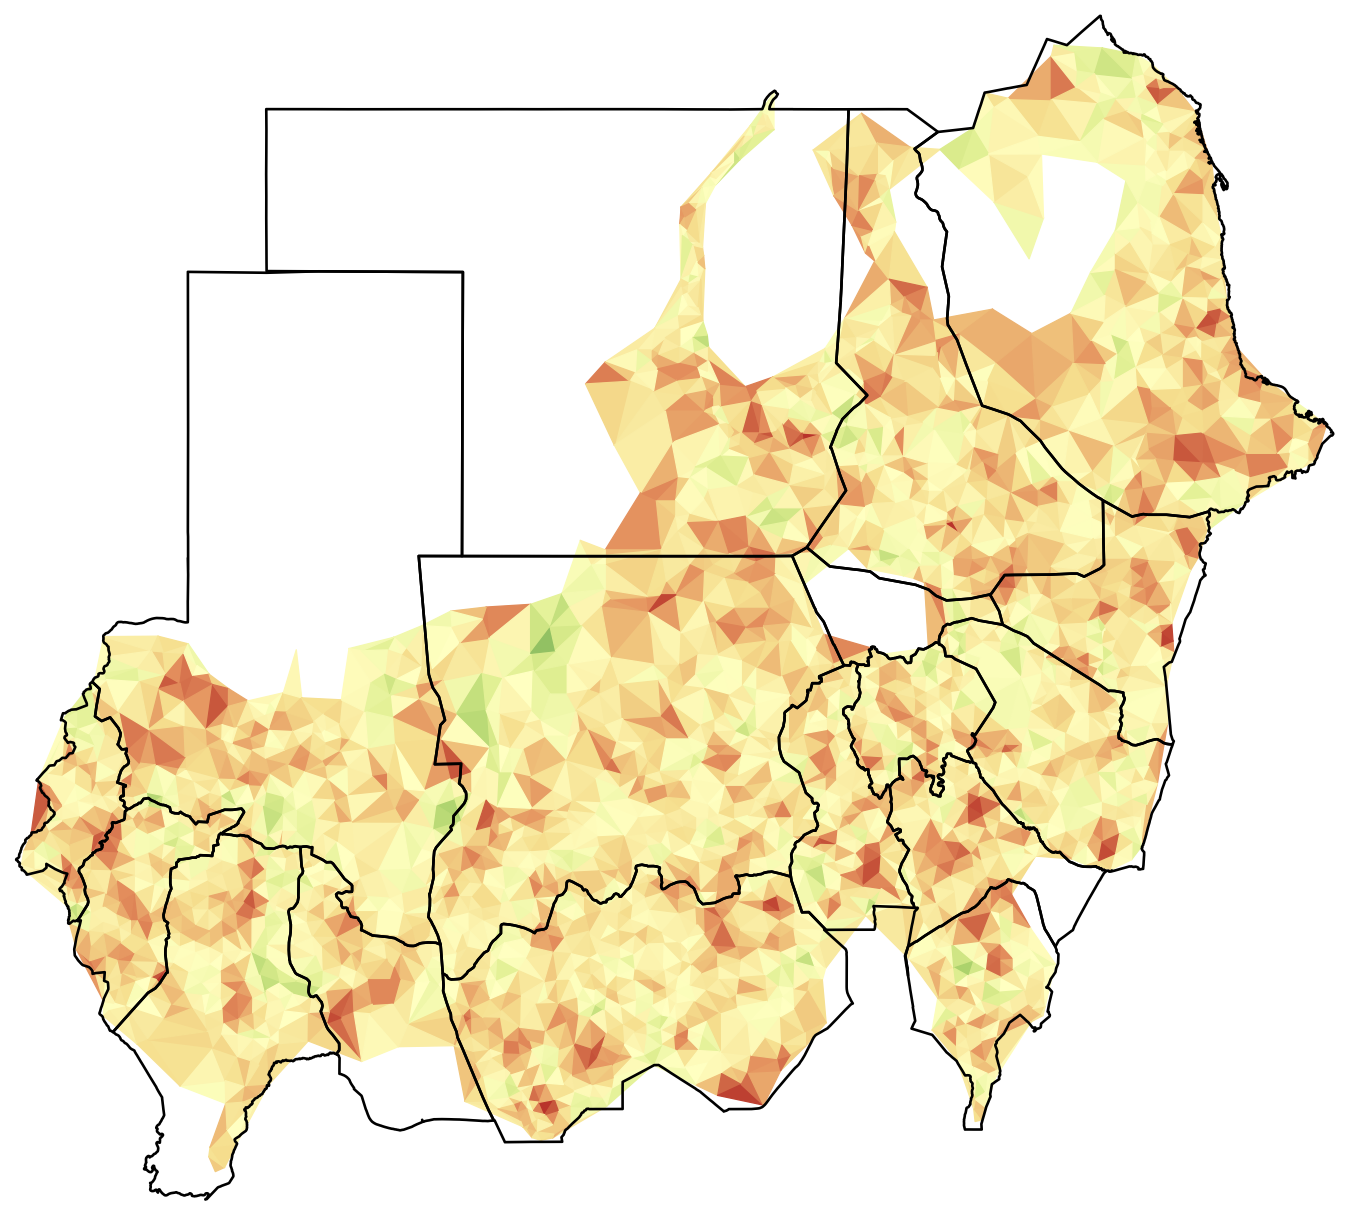
\includegraphics[width=18.75in]{figures/sudanMapTriSim} \end{center}

\hypertarget{exercise1}{%
\chapter{Retrieving map data in R}\label{exercise1}}

In this exercise we will use \textbf{R} to read a \textbf{shapefile}
dataset and get oriented with the structure and features of a
\textbf{shapefile} dataset. The aim of the exercise is for you to become
familiar with the use of R in handling \textbf{shapefile} datasets.

By this time, you have already learned how to issue a command to
retrieve a standard or typical dataset using the \texttt{read.table()}
function

For this exercise, we will use the \texttt{readOGR()} function provided
by the \texttt{rgdal} package to retrieve \textbf{shapefile} dateset.

First, we need to install and load the \texttt{rgdal} package.

~

\begin{Shaded}
\begin{Highlighting}[]
\KeywordTok{install.packages}\NormalTok{(“rgdal”)}
\KeywordTok{library}\NormalTok{(rgdal)}
\end{Highlighting}
\end{Shaded}

~

We can now try to read the Sudan \textbf{shapefile}. To do this however,
we need to have an orientation on what \textbf{shapefiles} are.

A \textbf{shapefile} is a digital vector storage format for storing
geometric location and associated attribute information. This format
lacks the capacity to store topological information. The
\textbf{shapefile} format was initially developed for proprietary use
with ArcView GIS version 2 in the early 1990s. It is now possible to
read and write \textbf{shapefiles} using a variety of programs including
data analysis software such as \textbf{R}.

\textbf{Shapefiles} are simple because they store the primitive
geometric data types of points, lines, and polygons. They are of limited
use without any attributes to specify what they represent. Therefore, a
table of records will store properties/attributes for each primitive
shape in the \textbf{shapefile}. Shapes (points/lines/polygons) together
with data attributes can create infinitely many representations about
geographic data. Representation provides the ability for powerful and
accurate computations.

While the term ``shapefile'' is quite common, a \textbf{shapefile} is
actually a set of several files. Three individual files are mandatory to
store the core data that comprise a \textbf{shapefile}:

\begin{itemize}
\tightlist
\item
  .shp
\item
  .shx
\item
  .dbf
\end{itemize}

The actual \textbf{shapefile} relates specifically to \texttt{.shp}
files but alone is incomplete for distribution, as the other supporting
files are required.

With this knowledge of \textbf{shapefiles}, let us now take a look at
the Sudan \textbf{shapefiles} dataset.

The Sudan \textbf{shapefiles} dataset contains the following
\textbf{shapefiles}:

~

\begin{longtable}[]{@{}lll@{}}
\caption{\label{tab:table1} Sudan shapefiles structure}\tabularnewline
\toprule
\begin{minipage}[b]{0.23\columnwidth}\raggedright
\textbf{Directory name}\strut
\end{minipage} & \begin{minipage}[b]{0.23\columnwidth}\raggedright
\textbf{Directory files}\strut
\end{minipage} & \begin{minipage}[b]{0.45\columnwidth}\raggedright
\textbf{Description}\strut
\end{minipage}\tabularnewline
\midrule
\endfirsthead
\toprule
\begin{minipage}[b]{0.23\columnwidth}\raggedright
\textbf{Directory name}\strut
\end{minipage} & \begin{minipage}[b]{0.23\columnwidth}\raggedright
\textbf{Directory files}\strut
\end{minipage} & \begin{minipage}[b]{0.45\columnwidth}\raggedright
\textbf{Description}\strut
\end{minipage}\tabularnewline
\midrule
\endhead
\begin{minipage}[t]{0.23\columnwidth}\raggedright
sudan01\strut
\end{minipage} & \begin{minipage}[t]{0.23\columnwidth}\raggedright
sudan01.shp sudan01.shx sudan01.dbf sudan01.prj sudan01.qpj\strut
\end{minipage} & \begin{minipage}[t]{0.45\columnwidth}\raggedright
Polygon shapefile of Sudan up to state administrative level\strut
\end{minipage}\tabularnewline
\begin{minipage}[t]{0.23\columnwidth}\raggedright
sudan02\strut
\end{minipage} & \begin{minipage}[t]{0.23\columnwidth}\raggedright
sudan02.shp sudan02.shx sudan02.dbf sudan02.prj sudan02.qpj\strut
\end{minipage} & \begin{minipage}[t]{0.45\columnwidth}\raggedright
Polygon shapefile of Sudan up to locality administrative level\strut
\end{minipage}\tabularnewline
\begin{minipage}[t]{0.23\columnwidth}\raggedright
grid12poly\strut
\end{minipage} & \begin{minipage}[t]{0.23\columnwidth}\raggedright
grid12poly.shp grid12poly.shx grid12poly.dbf grid12poly.prj
grid12poly.qpj\strut
\end{minipage} & \begin{minipage}[t]{0.45\columnwidth}\raggedright
Polygon shapefile of rectangular grid at d = 12km\strut
\end{minipage}\tabularnewline
\begin{minipage}[t]{0.23\columnwidth}\raggedright
grid12kmSudan\strut
\end{minipage} & \begin{minipage}[t]{0.23\columnwidth}\raggedright
grid12kmSudan.shp grid12kmSudan.shx grid12kmSudan.dbf grid12kmSudan.prj
grid12kmSudan.qpj\strut
\end{minipage} & \begin{minipage}[t]{0.45\columnwidth}\raggedright
Line shapefile of rectangular grid at d = 12km\strut
\end{minipage}\tabularnewline
\bottomrule
\end{longtable}

~

We can now retrieve these shapefile datasets and create an object for
each one using the \texttt{readOGR()} function from the \texttt{rgdal}
package.

~

\begin{Shaded}
\begin{Highlighting}[]
\NormalTok{sudan01 <-}\StringTok{ }\KeywordTok{readOGR}\NormalTok{(}\DataTypeTok{dsn =} \StringTok{"maps"}\NormalTok{, }\DataTypeTok{layer =} \StringTok{"sudan01"}\NormalTok{)}
\CommentTok{#> OGR data source with driver: ESRI Shapefile }
\CommentTok{#> Source: "/Users/ernest/Documents/GitHub/map-r/maps", layer: "sudan01"}
\CommentTok{#> with 18 features}
\CommentTok{#> It has 8 fields}

\NormalTok{sudan02 <-}\StringTok{ }\KeywordTok{readOGR}\NormalTok{(}\DataTypeTok{dsn =} \StringTok{"maps"}\NormalTok{, }\DataTypeTok{layer =} \StringTok{"sudan02"}\NormalTok{)}
\CommentTok{#> OGR data source with driver: ESRI Shapefile }
\CommentTok{#> Source: "/Users/ernest/Documents/GitHub/map-r/maps", layer: "sudan02"}
\CommentTok{#> with 169 features}
\CommentTok{#> It has 15 fields}

\NormalTok{grid12poly <-}\StringTok{ }\KeywordTok{readOGR}\NormalTok{(}\DataTypeTok{dsn =} \StringTok{"maps"}\NormalTok{, }\DataTypeTok{layer =} \StringTok{"grid12poly"}\NormalTok{)}
\CommentTok{#> OGR data source with driver: ESRI Shapefile }
\CommentTok{#> Source: "/Users/ernest/Documents/GitHub/map-r/maps", layer: "grid12poly"}
\CommentTok{#> with 13950 features}
\CommentTok{#> It has 5 fields}
\CommentTok{#> Integer64 fields read as strings:  ID}

\NormalTok{grid12kmSudan <-}\StringTok{ }\KeywordTok{readOGR}\NormalTok{(}\DataTypeTok{dsn =} \StringTok{"maps"}\NormalTok{, }\DataTypeTok{layer =} \StringTok{"grid12kmSudan"}\NormalTok{)}
\CommentTok{#> OGR data source with driver: ESRI Shapefile }
\CommentTok{#> Source: "/Users/ernest/Documents/GitHub/map-r/maps", layer: "grid12kmSudan"}
\CommentTok{#> with 245 features}
\CommentTok{#> It has 2 fields}
\CommentTok{#> Integer64 fields read as strings:  ID}
\end{Highlighting}
\end{Shaded}

~

This series of commands illustrates key things about the way shapefile
data can be read and handled in \textbf{R}.

First is that the retrieval of \textbf{shapefile} datasets follows a
very similar syntax as that of other standard datasets but just using
the \texttt{readOGR()} function. The same principles apply including
ensuring that you specify the corresponding directory in which your
\textbf{shapefiles} are stored.

Now that we have stored the various shapefile data into objects, we can
now explore and get ourselves oriented to the structure and features of
a \textbf{shapefile} data object. We will do this using standard / basic
functions in \textbf{R} that you have learned already in the previous
training.

First, let us learn the class of a \textbf{shapefile} data object. We
can find this out using the same function that you are familiar with
already and have used previously the \texttt{class()} function.

~

\begin{Shaded}
\begin{Highlighting}[]
\KeywordTok{class}\NormalTok{(sudan01)}
\end{Highlighting}
\end{Shaded}

~

This command gives the following output:

~

\begin{verbatim}
#> [1] "SpatialPolygonsDataFrame"
#> attr(,"package")
#> [1] "sp"
\end{verbatim}

~

This tells us that the \texttt{sudan01} object is of class
\texttt{SpatialPolygonsDataFrame}. It also tells us that this is a
special class specific to the \texttt{sp} package.

The \texttt{sp} package provides classes and methods for spatial data.
The classes document where the spatial location information resides, for
2D or 3D data. Utility functions are provided, e.g.~for plotting data as
maps, spatial selection, as well as methods for retrieving coordinates,
for subsetting, print, summary, etc.

If you check for the class of the other \textbf{shapefile} objects
you've created, you will see that all of them are of the same
\texttt{SpatialPolygonsDataFrame} class except for
\texttt{grid12kmSudan}. Checking for the class of \texttt{grid12kmSudan}
revealed the following:

~

\begin{Shaded}
\begin{Highlighting}[]
\KeywordTok{class}\NormalTok{(grid12kmSudan)}
\CommentTok{#> [1] "SpatialLinesDataFrame"}
\CommentTok{#> attr(,"package")}
\CommentTok{#> [1] "sp"}
\end{Highlighting}
\end{Shaded}

~

This tells us that the \texttt{grid12kmSudan} objects is of class
\texttt{SpatialLinesDataFrame}.

You are now getting introduced to two of the most common shapes of a
\textbf{shapefile}: \emph{polygons} and \emph{lines}.

A \emph{polygon} consists of one or more rings. A ring is a connected
sequence of four or more points that form a closed,
non-self-intersecting loop. A \emph{polygon} may contain multiple outer
rings. The order of vertices or orientation for a ring indicates which
side of the ring is the interior of the \emph{polygon}. The
neighbourhood to the right of an observer walking along the ring in
vertex order is the neighbourhood inside the \emph{polygon}. Vertices of
rings defining holes in \emph{polygons} are in a counterclockwise
direction. Vertices for a single, ringed \emph{polygon} are, therefore,
always in clockwise order. The rings of a \emph{polygon} are referred to
as its parts.

A \emph{line} is an ordered set of vertices that consists of one or more
parts. A part is a connected sequence of two or more points. Parts may
or may not be connected to one another. Parts may or may not intersect
one another.

One of the other shapes that \textbf{shapefiles} take or represent is
\emph{points}.

A \emph{point} consists of a pair of double-precision coordinates in the
order \texttt{x}, \texttt{y}.

Because of this simple property of a \emph{point} \textbf{shapefile}
(i.e.~a basic set of \texttt{x} and \texttt{y} coordinates), the use of
\textbf{shapefile} format to store the \emph{point} shape is not
commonly used. The \texttt{x} and \texttt{y} coordinates for
\emph{points} can be contained or stored in other more basic formats
such as CSV.

For example, the dataset that contains the \texttt{x} and \texttt{y}
coordinates of all the known villages in Sudan is named
\texttt{settlementsSudan.csv}. If we create an object called villages
for this dataset

~

\begin{Shaded}
\begin{Highlighting}[]
\NormalTok{villages <-}\StringTok{ }\KeywordTok{read.csv}\NormalTok{(}\StringTok{"maps/settlementsSudan.csv"}\NormalTok{, }\DataTypeTok{header =} \OtherTok{TRUE}\NormalTok{, }\DataTypeTok{sep =} \StringTok{","}\NormalTok{)}
\end{Highlighting}
\end{Shaded}

~

and use the \texttt{head()} function to view the first 10 rows of this
dataset

~

\begin{Shaded}
\begin{Highlighting}[]
\KeywordTok{head}\NormalTok{(villages, }\DecValTok{10}\NormalTok{)}
\end{Highlighting}
\end{Shaded}

~

we get:

~

\begin{verbatim}
#>    ID      Village Pop     Source      State Locality        X        Y
#> 1   1        Kosti         Georef White Nile    Kosti 32.66751 13.14846
#> 2   2     Tandalti     Calculated White Nile    Kosti 31.86393 13.00969
#> 3   3    Qawz kobi            GPS White Nile    Kosti 32.35000 13.60000
#> 4   4    Karjuggle            GPS White Nile    Kosti 32.38333 13.46667
#> 5   5   Idd maktuf            GPS White Nile    Kosti 32.28333 13.50000
#> 6   6       Maryam            GPS White Nile    Kosti 32.55000 13.46667
#> 7   7 Qawz nyaneir            GPS White Nile    Kosti 32.28333 13.60000
#> 8   8       Salogi            GPS White Nile    Kosti 32.45000 13.15000
#> 9   9      Sulayah            GPS White Nile    Kosti 32.25000 13.26667
#> 10 10      Seleima     Calculated White Nile    Kosti 32.05833 13.00833
#>    Remarks
#> 1         
#> 2         
#> 3         
#> 4         
#> 5         
#> 6         
#> 7         
#> 8         
#> 9         
#> 10
\end{verbatim}

~

As you will notice here, the villages object contains information on the
\texttt{x} and \texttt{y} coordinates of each of the villages in Sudan.
So, whilst this dataset is not a \textbf{shapefile} (it is a basic data
frame), it has information and a structure that is comparable to a point
\textbf{shapefile} as defined above.

In the succeeding exercises, this similarity of a \emph{point}
\textbf{shapefile} and a standard data frame containing \texttt{x} and
\texttt{y} coordinates of \emph{points} will be further discussed and
illuminated.

This knowledge on classes and shapes of \textbf{shapefiles} is an
important learning particularly when performing functions to handle or
manipulate different \textbf{shapefile} objects. The general principle
is that functions or operations between two or more \textbf{shapefile}
objects require these objects to be of the same class or family of
classes. Also, the shapes defined by the \textbf{shapefile} object
determine the way the \textbf{shapefile} data is structured which in
turn determine how these objects can and should be handled or
manipulated in \textbf{R}. These principles will be further illuminated
in the succeeding exercises.

After learning about the class of \textbf{shapefile} objects, we now
learn about the structure of these objects. We are able to appreciate
the structure of a \textbf{shapefile} object by using the function
\texttt{str()}.

~

\begin{Shaded}
\begin{Highlighting}[]
\KeywordTok{str}\NormalTok{(sudan01)}
\end{Highlighting}
\end{Shaded}

~

The output of this command is:

~

\begin{verbatim}
#> Formal class 'SpatialPolygonsDataFrame' [package "sp"] with 5 slots
#>   ..@ data       :'data.frame':  18 obs. of  8 variables:
#>   .. ..$ State     : chr [1:18] "West Darfur" "Central Darfur" "North Darfur" "East Darfur" ...
#>   .. ..$ Old_state : chr [1:18] "West Darfur" "West Darfur" "North Darfur" "South Darfur" ...
#>   .. ..$ New_State : chr [1:18] "West Darfur" "Central Darfur" "North Darfur" "East Darfur" ...
#>   .. ..$ STATE_1   : chr [1:18] NA NA NA NA ...
#>   .. ..$ STATEAR   : chr [1:18] NA NA NA NA ...
#>   .. ..$ Source    : chr [1:18] NA NA NA NA ...
#>   .. ..$ STATE_CODE: chr [1:18] NA NA NA NA ...
#>   .. ..$ ISO_CODE  : chr [1:18] NA NA NA NA ...
#>   ..@ polygons   :List of 18
#>   .. ..$ :Formal class 'Polygons' [package "sp"] with 5 slots
#>   .. .. .. ..@ Polygons :List of 1
#>   .. .. .. .. ..$ :Formal class 'Polygon' [package "sp"] with 5 slots
#>   .. .. .. .. .. .. ..@ labpt  : num [1:2] 22.6 13.5
#>   .. .. .. .. .. .. ..@ area   : num 1.86
#>   .. .. .. .. .. .. ..@ hole   : logi FALSE
#>   .. .. .. .. .. .. ..@ ringDir: int 1
#>   .. .. .. .. .. .. ..@ coords : num [1:981, 1:2] 22.1 22.1 22.1 22.2 22.2 ...
#>   .. .. .. ..@ plotOrder: int 1
#>   .. .. .. ..@ labpt    : num [1:2] 22.6 13.5
#>   .. .. .. ..@ ID       : chr "0"
#>   .. .. .. ..@ area     : num 1.86
#>   .. ..$ :Formal class 'Polygons' [package "sp"] with 5 slots
#>   .. .. .. ..@ Polygons :List of 1
#>   .. .. .. .. ..$ :Formal class 'Polygon' [package "sp"] with 5 slots
#>   .. .. .. .. .. .. ..@ labpt  : num [1:2] 23.4 12.3
#>   .. .. .. .. .. .. ..@ area   : num 2.75
#>   .. .. .. .. .. .. ..@ hole   : logi FALSE
#>   .. .. .. .. .. .. ..@ ringDir: int 1
#>   .. .. .. .. .. .. ..@ coords : num [1:463, 1:2] 23.6 23.6 23.6 23.6 23.7 ...
#>   .. .. .. ..@ plotOrder: int 1
#>   .. .. .. ..@ labpt    : num [1:2] 23.4 12.3
#>   .. .. .. ..@ ID       : chr "1"
#>   .. .. .. ..@ area     : num 2.75
#>   .. ..$ :Formal class 'Polygons' [package "sp"] with 5 slots
#>   .. .. .. ..@ Polygons :List of 1
#>   .. .. .. .. ..$ :Formal class 'Polygon' [package "sp"] with 5 slots
#>   .. .. .. .. .. .. ..@ labpt  : num [1:2] 25.6 16.2
#>   .. .. .. .. .. .. ..@ area   : num 26.7
#>   .. .. .. .. .. .. ..@ hole   : logi FALSE
#>   .. .. .. .. .. .. ..@ ringDir: int 1
#>   .. .. .. .. .. .. ..@ coords : num [1:669, 1:2] 27.5 27.5 27.2 27.1 26.9 ...
#>   .. .. .. ..@ plotOrder: int 1
#>   .. .. .. ..@ labpt    : num [1:2] 25.6 16.2
#>   .. .. .. ..@ ID       : chr "2"
#>   .. .. .. ..@ area     : num 26.7
#>   .. ..$ :Formal class 'Polygons' [package "sp"] with 5 slots
#>   .. .. .. ..@ Polygons :List of 1
#>   .. .. .. .. ..$ :Formal class 'Polygon' [package "sp"] with 5 slots
#>   .. .. .. .. .. .. ..@ labpt  : num [1:2] 26.5 11
#>   .. .. .. .. .. .. ..@ area   : num 4.44
#>   .. .. .. .. .. .. ..@ hole   : logi FALSE
#>   .. .. .. .. .. .. ..@ ringDir: int 1
#>   .. .. .. .. .. .. ..@ coords : num [1:932, 1:2] 25.5 25.6 25.6 25.6 25.6 ...
#>   .. .. .. ..@ plotOrder: int 1
#>   .. .. .. ..@ labpt    : num [1:2] 26.5 11
#>   .. .. .. ..@ ID       : chr "3"
#>   .. .. .. ..@ area     : num 4.44
#>   .. ..$ :Formal class 'Polygons' [package "sp"] with 5 slots
#>   .. .. .. ..@ Polygons :List of 1
#>   .. .. .. .. ..$ :Formal class 'Polygon' [package "sp"] with 5 slots
#>   .. .. .. .. .. .. ..@ labpt  : num [1:2] 24.4 11
#>   .. .. .. .. .. .. ..@ area   : num 6.91
#>   .. .. .. .. .. .. ..@ hole   : logi FALSE
#>   .. .. .. .. .. .. ..@ ringDir: int 1
#>   .. .. .. .. .. .. ..@ coords : num [1:1896, 1:2] 24.4 24.4 24.4 24.4 24.4 ...
#>   .. .. .. ..@ plotOrder: int 1
#>   .. .. .. ..@ labpt    : num [1:2] 24.4 11
#>   .. .. .. ..@ ID       : chr "4"
#>   .. .. .. ..@ area     : num 6.91
#>   .. ..$ :Formal class 'Polygons' [package "sp"] with 5 slots
#>   .. .. .. ..@ Polygons :List of 1
#>   .. .. .. .. ..$ :Formal class 'Polygon' [package "sp"] with 5 slots
#>   .. .. .. .. .. .. ..@ labpt  : num [1:2] 33.3 14.6
#>   .. .. .. .. .. .. ..@ area   : num 2.28
#>   .. .. .. .. .. .. ..@ hole   : logi FALSE
#>   .. .. .. .. .. .. ..@ ringDir: int 1
#>   .. .. .. .. .. .. ..@ coords : num [1:490, 1:2] 33.6 33.6 33.6 33.6 33.6 ...
#>   .. .. .. ..@ plotOrder: int 1
#>   .. .. .. ..@ labpt    : num [1:2] 33.3 14.6
#>   .. .. .. ..@ ID       : chr "5"
#>   .. .. .. ..@ area     : num 2.28
#>   .. ..$ :Formal class 'Polygons' [package "sp"] with 5 slots
#>   .. .. .. ..@ Polygons :List of 1
#>   .. .. .. .. ..$ :Formal class 'Polygon' [package "sp"] with 5 slots
#>   .. .. .. .. .. .. ..@ labpt  : num [1:2] 34.1 11.3
#>   .. .. .. .. .. .. ..@ area   : num 3.16
#>   .. .. .. .. .. .. ..@ hole   : logi FALSE
#>   .. .. .. .. .. .. ..@ ringDir: int 1
#>   .. .. .. .. .. .. ..@ coords : num [1:406, 1:2] 34.5 34.5 34.5 34.5 34.5 ...
#>   .. .. .. ..@ plotOrder: int 1
#>   .. .. .. ..@ labpt    : num [1:2] 34.1 11.3
#>   .. .. .. ..@ ID       : chr "6"
#>   .. .. .. ..@ area     : num 3.16
#>   .. ..$ :Formal class 'Polygons' [package "sp"] with 5 slots
#>   .. .. .. ..@ Polygons :List of 1
#>   .. .. .. .. ..$ :Formal class 'Polygon' [package "sp"] with 5 slots
#>   .. .. .. .. .. .. ..@ labpt  : num [1:2] 35.1 14.2
#>   .. .. .. .. .. .. ..@ area   : num 4.99
#>   .. .. .. .. .. .. ..@ hole   : logi FALSE
#>   .. .. .. .. .. .. ..@ ringDir: int 1
#>   .. .. .. .. .. .. ..@ coords : num [1:505, 1:2] 34.2 34.3 34.4 34.4 34.5 ...
#>   .. .. .. ..@ plotOrder: int 1
#>   .. .. .. ..@ labpt    : num [1:2] 35.1 14.2
#>   .. .. .. ..@ ID       : chr "7"
#>   .. .. .. ..@ area     : num 4.99
#>   .. ..$ :Formal class 'Polygons' [package "sp"] with 5 slots
#>   .. .. .. ..@ Polygons :List of 1
#>   .. .. .. .. ..$ :Formal class 'Polygon' [package "sp"] with 5 slots
#>   .. .. .. .. .. .. ..@ labpt  : num [1:2] 35.9 15.8
#>   .. .. .. .. .. .. ..@ area   : num 4.1
#>   .. .. .. .. .. .. ..@ hole   : logi FALSE
#>   .. .. .. .. .. .. ..@ ringDir: int 1
#>   .. .. .. .. .. .. ..@ coords : num [1:294, 1:2] 35.7 36 36.1 36.2 36.2 ...
#>   .. .. .. ..@ plotOrder: int 1
#>   .. .. .. ..@ labpt    : num [1:2] 35.9 15.8
#>   .. .. .. ..@ ID       : chr "8"
#>   .. .. .. ..@ area     : num 4.1
#>   .. ..$ :Formal class 'Polygons' [package "sp"] with 5 slots
#>   .. .. .. ..@ Polygons :List of 1
#>   .. .. .. .. ..$ :Formal class 'Polygon' [package "sp"] with 5 slots
#>   .. .. .. .. .. .. ..@ labpt  : num [1:2] 32.8 15.9
#>   .. .. .. .. .. .. ..@ area   : num 1.79
#>   .. .. .. .. .. .. ..@ hole   : logi FALSE
#>   .. .. .. .. .. .. ..@ ringDir: int 1
#>   .. .. .. .. .. .. ..@ coords : num [1:198, 1:2] 33.5 33.7 34 34 34 ...
#>   .. .. .. ..@ plotOrder: int 1
#>   .. .. .. ..@ labpt    : num [1:2] 32.8 15.9
#>   .. .. .. ..@ ID       : chr "9"
#>   .. .. .. ..@ area     : num 1.79
#>   .. ..$ :Formal class 'Polygons' [package "sp"] with 5 slots
#>   .. .. .. ..@ Polygons :List of 1
#>   .. .. .. .. ..$ :Formal class 'Polygon' [package "sp"] with 5 slots
#>   .. .. .. .. .. .. ..@ labpt  : num [1:2] 33.5 18.3
#>   .. .. .. .. .. .. ..@ area   : num 11.1
#>   .. .. .. .. .. .. ..@ hole   : logi FALSE
#>   .. .. .. .. .. .. ..@ ringDir: int 1
#>   .. .. .. .. .. .. ..@ coords : num [1:226, 1:2] 35.6 35.4 35.4 35.3 35.3 ...
#>   .. .. .. ..@ plotOrder: int 1
#>   .. .. .. ..@ labpt    : num [1:2] 33.5 18.3
#>   .. .. .. ..@ ID       : chr "10"
#>   .. .. .. ..@ area     : num 11.1
#>   .. ..$ :Formal class 'Polygons' [package "sp"] with 5 slots
#>   .. .. .. ..@ Polygons :List of 1
#>   .. .. .. .. ..$ :Formal class 'Polygon' [package "sp"] with 5 slots
#>   .. .. .. .. .. .. ..@ labpt  : num [1:2] 29.3 19.6
#>   .. .. .. .. .. .. ..@ area   : num 31.4
#>   .. .. .. .. .. .. ..@ hole   : logi FALSE
#>   .. .. .. .. .. .. ..@ ringDir: int 1
#>   .. .. .. .. .. .. ..@ coords : num [1:117, 1:2] 31.7 32.1 32.1 32.4 32.4 ...
#>   .. .. .. ..@ plotOrder: int 1
#>   .. .. .. ..@ labpt    : num [1:2] 29.3 19.6
#>   .. .. .. ..@ ID       : chr "11"
#>   .. .. .. ..@ area     : num 31.4
#>   .. ..$ :Formal class 'Polygons' [package "sp"] with 5 slots
#>   .. .. .. ..@ Polygons :List of 1
#>   .. .. .. .. ..$ :Formal class 'Polygon' [package "sp"] with 5 slots
#>   .. .. .. .. .. .. ..@ labpt  : num [1:2] 35.7 19.8
#>   .. .. .. .. .. .. ..@ area   : num 18.6
#>   .. .. .. .. .. .. ..@ hole   : logi FALSE
#>   .. .. .. .. .. .. ..@ ringDir: int 1
#>   .. .. .. .. .. .. ..@ coords : num [1:2309, 1:2] 37 37 37 37 37 ...
#>   .. .. .. ..@ plotOrder: int 1
#>   .. .. .. ..@ labpt    : num [1:2] 35.7 19.8
#>   .. .. .. ..@ ID       : chr "12"
#>   .. .. .. ..@ area     : num 18.6
#>   .. ..$ :Formal class 'Polygons' [package "sp"] with 5 slots
#>   .. .. .. ..@ Polygons :List of 2
#>   .. .. .. .. ..$ :Formal class 'Polygon' [package "sp"] with 5 slots
#>   .. .. .. .. .. .. ..@ labpt  : num [1:2] 33.2 11.5
#>   .. .. .. .. .. .. ..@ area   : num 0.00152
#>   .. .. .. .. .. .. ..@ hole   : logi FALSE
#>   .. .. .. .. .. .. ..@ ringDir: int 1
#>   .. .. .. .. .. .. ..@ coords : num [1:10, 1:2] 33.2 33.2 33.2 33.1 33.1 ...
#>   .. .. .. .. ..$ :Formal class 'Polygon' [package "sp"] with 5 slots
#>   .. .. .. .. .. .. ..@ labpt  : num [1:2] 34 12.9
#>   .. .. .. .. .. .. ..@ area   : num 3.27
#>   .. .. .. .. .. .. ..@ hole   : logi FALSE
#>   .. .. .. .. .. .. ..@ ringDir: int 1
#>   .. .. .. .. .. .. ..@ coords : num [1:545, 1:2] 33.9 33.9 33.9 33.9 33.9 ...
#>   .. .. .. ..@ plotOrder: int [1:2] 2 1
#>   .. .. .. ..@ labpt    : num [1:2] 34 12.9
#>   .. .. .. ..@ ID       : chr "13"
#>   .. .. .. ..@ area     : num 3.27
#>   .. ..$ :Formal class 'Polygons' [package "sp"] with 5 slots
#>   .. .. .. ..@ Polygons :List of 1
#>   .. .. .. .. ..$ :Formal class 'Polygon' [package "sp"] with 5 slots
#>   .. .. .. .. .. .. ..@ labpt  : num [1:2] 32.3 13.4
#>   .. .. .. .. .. .. ..@ area   : num 3.17
#>   .. .. .. .. .. .. ..@ hole   : logi FALSE
#>   .. .. .. .. .. .. ..@ ringDir: int 1
#>   .. .. .. .. .. .. ..@ coords : num [1:378, 1:2] 32.5 32.5 32.5 32.5 32.5 ...
#>   .. .. .. ..@ plotOrder: int 1
#>   .. .. .. ..@ labpt    : num [1:2] 32.3 13.4
#>   .. .. .. ..@ ID       : chr "14"
#>   .. .. .. ..@ area     : num 3.17
#>   .. ..$ :Formal class 'Polygons' [package "sp"] with 5 slots
#>   .. .. .. ..@ Polygons :List of 1
#>   .. .. .. .. ..$ :Formal class 'Polygon' [package "sp"] with 5 slots
#>   .. .. .. .. .. .. ..@ labpt  : num [1:2] 30.8 11.3
#>   .. .. .. .. .. .. ..@ area   : num 6.49
#>   .. .. .. .. .. .. ..@ hole   : logi FALSE
#>   .. .. .. .. .. .. ..@ ringDir: int 1
#>   .. .. .. .. .. .. ..@ coords : num [1:451, 1:2] 31.7 31.7 31.7 31.7 31.7 ...
#>   .. .. .. ..@ plotOrder: int 1
#>   .. .. .. ..@ labpt    : num [1:2] 30.8 11.3
#>   .. .. .. ..@ ID       : chr "15"
#>   .. .. .. ..@ area     : num 6.49
#>   .. ..$ :Formal class 'Polygons' [package "sp"] with 5 slots
#>   .. .. .. ..@ Polygons :List of 1
#>   .. .. .. .. ..$ :Formal class 'Polygon' [package "sp"] with 5 slots
#>   .. .. .. .. .. .. ..@ labpt  : num [1:2] 28.4 11.8
#>   .. .. .. .. .. .. ..@ area   : num 9.47
#>   .. .. .. .. .. .. ..@ hole   : logi FALSE
#>   .. .. .. .. .. .. ..@ ringDir: int 1
#>   .. .. .. .. .. .. ..@ coords : num [1:566, 1:2] 27.5 27.5 27.5 27.5 27.8 ...
#>   .. .. .. ..@ plotOrder: int 1
#>   .. .. .. ..@ labpt    : num [1:2] 28.4 11.8
#>   .. .. .. ..@ ID       : chr "16"
#>   .. .. .. ..@ area     : num 9.47
#>   .. ..$ :Formal class 'Polygons' [package "sp"] with 5 slots
#>   .. .. .. ..@ Polygons :List of 1
#>   .. .. .. .. ..$ :Formal class 'Polygon' [package "sp"] with 5 slots
#>   .. .. .. .. .. .. ..@ labpt  : num [1:2] 29.7 14.8
#>   .. .. .. .. .. .. ..@ area   : num 15.7
#>   .. .. .. .. .. .. ..@ hole   : logi FALSE
#>   .. .. .. .. .. .. ..@ ringDir: int 1
#>   .. .. .. .. .. .. ..@ coords : num [1:385, 1:2] 26.9 27.1 27.2 27.5 28.6 ...
#>   .. .. .. ..@ plotOrder: int 1
#>   .. .. .. ..@ labpt    : num [1:2] 29.7 14.8
#>   .. .. .. ..@ ID       : chr "17"
#>   .. .. .. ..@ area     : num 15.7
#>   ..@ plotOrder  : int [1:18] 12 3 13 18 11 17 5 16 8 4 ...
#>   ..@ bbox       : num [1:2, 1:2] 21.81 8.64 38.59 23.14
#>   .. ..- attr(*, "dimnames")=List of 2
#>   .. .. ..$ : chr [1:2] "x" "y"
#>   .. .. ..$ : chr [1:2] "min" "max"
#>   ..@ proj4string:Formal class 'CRS' [package "sp"] with 1 slot
#>   .. .. ..@ projargs: chr "+proj=longlat +datum=WGS84 +no_defs +ellps=WGS84 +towgs84=0,0,0"
\end{verbatim}

~

which gives the class of the \textbf{shapefile} object and gives us an
idea of the data structure as having 5 slots. This is one of the key
differences of a \texttt{sp} data frame compared to a standard basic
data frame. In a basic data frame, you basically have single data set
organised in rows and columns similar to that of a table. In a
\texttt{sp} data frame, you can think of it as a compound data frame in
which each slot contains a specific dataset.

As you look further down into the structure of the \textbf{shapefile}
object, you will notice the \texttt{@} symbol recurring 5 times. This is
the symbol used to retrieve the different slots of the
\textbf{shapefile} objects.

\newpage

The 5 slots in a \texttt{SpatialPolygonsDataFrame} are:

~

\begin{longtable}[]{@{}ll@{}}
\caption{\label{tab:table2} SpatialPolygonsDataFrame
structure}\tabularnewline
\toprule
\begin{minipage}[t]{0.32\columnwidth}\raggedright
\textbf{data}\strut
\end{minipage} & \begin{minipage}[t]{0.62\columnwidth}\raggedright
Contains the index or reference data frame of the \textbf{shapefile} the
number of rows of which indicates the number of polygons that comprise
the entire \textbf{shapefile}.\strut
\end{minipage}\tabularnewline
\begin{minipage}[t]{0.32\columnwidth}\raggedright
\textbf{polygons}\strut
\end{minipage} & \begin{minipage}[t]{0.62\columnwidth}\raggedright
Contains \emph{n} number of datasets based on the number of
\emph{polygons} that comprise the entire \textbf{shapefile}.\strut
\end{minipage}\tabularnewline
\begin{minipage}[t]{0.32\columnwidth}\raggedright
\textbf{plotOrder}\strut
\end{minipage} & \begin{minipage}[t]{0.62\columnwidth}\raggedright
Contains an integer vector with a length equal to the number of
\emph{polygons} that comprise the entire \textbf{shapefile} and have
values starting from 1 to \emph{n} number of \emph{polygons} in the
entire \textbf{shapefile}. The order of the values of this vector
determines which \emph{polygon} is drawn first when plotting. This order
is determined by decreasing area size of the \emph{polygons}.\strut
\end{minipage}\tabularnewline
\begin{minipage}[t]{0.32\columnwidth}\raggedright
\textbf{bbox}\strut
\end{minipage} & \begin{minipage}[t]{0.62\columnwidth}\raggedright
Contains a matrix the values of which are the minimum and maximum
\texttt{x} and \texttt{y} limits of the entire \textbf{shapefile}.\strut
\end{minipage}\tabularnewline
\begin{minipage}[t]{0.32\columnwidth}\raggedright
\textbf{proj4string}\strut
\end{minipage} & \begin{minipage}[t]{0.62\columnwidth}\raggedright
Contains a character string that specifies the projection and datum of
the \textbf{shapefile} object\strut
\end{minipage}\tabularnewline
\bottomrule
\end{longtable}

~

Now let us try to extract the different slots of \texttt{sudan01}
object. Making a call for the \texttt{data} slot gives:

~

\begin{Shaded}
\begin{Highlighting}[]
\NormalTok{sudan01}\OperatorTok{@}\NormalTok{data}
\CommentTok{#>                State         Old_state         New_State STATE_1 STATEAR}
\CommentTok{#> 0        West Darfur       West Darfur       West Darfur    <NA>    <NA>}
\CommentTok{#> 1     Central Darfur       West Darfur    Central Darfur    <NA>    <NA>}
\CommentTok{#> 2       North Darfur      North Darfur      North Darfur    <NA>    <NA>}
\CommentTok{#> 3        East Darfur      South Darfur       East Darfur    <NA>    <NA>}
\CommentTok{#> 4       South Darfur      South Darfur      South Darfur    <NA>    <NA>}
\CommentTok{#> 5          Al Gezira              <NA>              <NA>    <NA>    <NA>}
\CommentTok{#> 6          Blue Nile              <NA>              <NA>    <NA>    <NA>}
\CommentTok{#> 7            Gedaref              <NA>              <NA>    <NA>    <NA>}
\CommentTok{#> 8            Kassala              <NA>              <NA>    <NA>    <NA>}
\CommentTok{#> 9           Khartoum              <NA>              <NA>    <NA>    <NA>}
\CommentTok{#> 10              Nile              <NA>              <NA>    <NA>    <NA>}
\CommentTok{#> 11          Northern              <NA>              <NA>    <NA>    <NA>}
\CommentTok{#> 12           Red Sea              <NA>              <NA>    <NA>    <NA>}
\CommentTok{#> 13            Sennar              <NA>              <NA>    <NA>    <NA>}
\CommentTok{#> 14        White Nile              <NA>              <NA>    <NA>    <NA>}
\CommentTok{#> 15 Southern Kordofan Southern Kordofan Southern Kordofan    <NA>    <NA>}
\CommentTok{#> 16  Western Kordofan    South Kordofan  Western Kordofan    <NA>    <NA>}
\CommentTok{#> 17 Northern Kordofan Northern Kordofan Northern Kordofan    <NA>    <NA>}
\CommentTok{#>    Source STATE_CODE ISO_CODE}
\CommentTok{#> 0    <NA>       <NA>     <NA>}
\CommentTok{#> 1    <NA>       <NA>     <NA>}
\CommentTok{#> 2    <NA>       <NA>     <NA>}
\CommentTok{#> 3    <NA>       <NA>     <NA>}
\CommentTok{#> 4    <NA>       <NA>     <NA>}
\CommentTok{#> 5     CBS       SU04    SD-07}
\CommentTok{#> 6     CBS       SU02    SD-24}
\CommentTok{#> 7     CBS       SU05    SD-06}
\CommentTok{#> 8     CBS       SU07    SD-05}
\CommentTok{#> 9     CBS       SU08    SD-03}
\CommentTok{#> 10    CBS       SU10    SD-04}
\CommentTok{#> 11    CBS       SU11    SD-01}
\CommentTok{#> 12    CBS       SU15    SD-26}
\CommentTok{#> 13    CBS       SU16    SD-25}
\CommentTok{#> 14    CBS       SU25    SD-08}
\CommentTok{#> 15   <NA>       <NA>     <NA>}
\CommentTok{#> 16   <NA>       <NA>     <NA>}
\CommentTok{#> 17   <NA>       <NA>     <NA>}
\end{Highlighting}
\end{Shaded}

~

Here we note that the \texttt{sudan01} \textbf{shapefile} contains
\emph{polygons} of the each of the states of Sudan with
\texttt{sudan01@data} specifying the names of each of these states.

To check for the number of \emph{polygons} in \texttt{sudan01}
\textbf{shapefile} (the answer to which will also be the number of
states in Sudan), we can use the \texttt{nrow()} function as follows:

~

\begin{Shaded}
\begin{Highlighting}[]
\KeywordTok{nrow}\NormalTok{(sudan01}\OperatorTok{@}\NormalTok{data)}
\end{Highlighting}
\end{Shaded}

\newpage

which gives a result of

~

\begin{verbatim}
#> [1] 18
\end{verbatim}

~

There are 18 polygons in \texttt{sudan01} \textbf{shapefile} which
indicate that Sudan has about 18 states (if the \textbf{shapefile} used
is up-to-date).

Let us now try extract the \emph{polygons} slot of \texttt{sudan01}. If
we make a call for the \emph{polygons} slot as below:

~

\begin{Shaded}
\begin{Highlighting}[]
\NormalTok{sudan01}\OperatorTok{@}\NormalTok{polygons}
\end{Highlighting}
\end{Shaded}

~

we end up with a very long output which is not easy to review or
appreciate. This is understandable because from the previous command
extracting the slot data of \texttt{sudan01} we know already that the
\emph{polygons} slot will have 18 sets of \emph{polygon}
\textbf{shapefile} data each of which will have it's own datasets and
data structure. This means that the output will be very long and not
easy to manage.

In this instance, a review of the structure of \texttt{sudan01@polygons}
may help in getting an insight as to how to handle or manage the
datasets contained inside this slot. We call the \texttt{str()} function
on \texttt{sudan01@polygons} as follows:

~

\begin{Shaded}
\begin{Highlighting}[]
\KeywordTok{str}\NormalTok{(sudan01}\OperatorTok{@}\NormalTok{polygons)}
\CommentTok{#> List of 18}
\CommentTok{#>  $ :Formal class 'Polygons' [package "sp"] with 5 slots}
\CommentTok{#>   .. ..@ Polygons :List of 1}
\CommentTok{#>   .. .. ..$ :Formal class 'Polygon' [package "sp"] with 5 slots}
\CommentTok{#>   .. .. .. .. ..@ labpt  : num [1:2] 22.6 13.5}
\CommentTok{#>   .. .. .. .. ..@ area   : num 1.86}
\CommentTok{#>   .. .. .. .. ..@ hole   : logi FALSE}
\CommentTok{#>   .. .. .. .. ..@ ringDir: int 1}
\CommentTok{#>   .. .. .. .. ..@ coords : num [1:981, 1:2] 22.1 22.1 22.1 22.2 22.2 ...}
\CommentTok{#>   .. ..@ plotOrder: int 1}
\CommentTok{#>   .. ..@ labpt    : num [1:2] 22.6 13.5}
\CommentTok{#>   .. ..@ ID       : chr "0"}
\CommentTok{#>   .. ..@ area     : num 1.86}
\CommentTok{#>  $ :Formal class 'Polygons' [package "sp"] with 5 slots}
\CommentTok{#>   .. ..@ Polygons :List of 1}
\CommentTok{#>   .. .. ..$ :Formal class 'Polygon' [package "sp"] with 5 slots}
\CommentTok{#>   .. .. .. .. ..@ labpt  : num [1:2] 23.4 12.3}
\CommentTok{#>   .. .. .. .. ..@ area   : num 2.75}
\CommentTok{#>   .. .. .. .. ..@ hole   : logi FALSE}
\CommentTok{#>   .. .. .. .. ..@ ringDir: int 1}
\CommentTok{#>   .. .. .. .. ..@ coords : num [1:463, 1:2] 23.6 23.6 23.6 23.6 23.7 ...}
\CommentTok{#>   .. ..@ plotOrder: int 1}
\CommentTok{#>   .. ..@ labpt    : num [1:2] 23.4 12.3}
\CommentTok{#>   .. ..@ ID       : chr "1"}
\CommentTok{#>   .. ..@ area     : num 2.75}
\CommentTok{#>  $ :Formal class 'Polygons' [package "sp"] with 5 slots}
\CommentTok{#>   .. ..@ Polygons :List of 1}
\CommentTok{#>   .. .. ..$ :Formal class 'Polygon' [package "sp"] with 5 slots}
\CommentTok{#>   .. .. .. .. ..@ labpt  : num [1:2] 25.6 16.2}
\CommentTok{#>   .. .. .. .. ..@ area   : num 26.7}
\CommentTok{#>   .. .. .. .. ..@ hole   : logi FALSE}
\CommentTok{#>   .. .. .. .. ..@ ringDir: int 1}
\CommentTok{#>   .. .. .. .. ..@ coords : num [1:669, 1:2] 27.5 27.5 27.2 27.1 26.9 ...}
\CommentTok{#>   .. ..@ plotOrder: int 1}
\CommentTok{#>   .. ..@ labpt    : num [1:2] 25.6 16.2}
\CommentTok{#>   .. ..@ ID       : chr "2"}
\CommentTok{#>   .. ..@ area     : num 26.7}
\CommentTok{#>  $ :Formal class 'Polygons' [package "sp"] with 5 slots}
\CommentTok{#>   .. ..@ Polygons :List of 1}
\CommentTok{#>   .. .. ..$ :Formal class 'Polygon' [package "sp"] with 5 slots}
\CommentTok{#>   .. .. .. .. ..@ labpt  : num [1:2] 26.5 11}
\CommentTok{#>   .. .. .. .. ..@ area   : num 4.44}
\CommentTok{#>   .. .. .. .. ..@ hole   : logi FALSE}
\CommentTok{#>   .. .. .. .. ..@ ringDir: int 1}
\CommentTok{#>   .. .. .. .. ..@ coords : num [1:932, 1:2] 25.5 25.6 25.6 25.6 25.6 ...}
\CommentTok{#>   .. ..@ plotOrder: int 1}
\CommentTok{#>   .. ..@ labpt    : num [1:2] 26.5 11}
\CommentTok{#>   .. ..@ ID       : chr "3"}
\CommentTok{#>   .. ..@ area     : num 4.44}
\CommentTok{#>  $ :Formal class 'Polygons' [package "sp"] with 5 slots}
\CommentTok{#>   .. ..@ Polygons :List of 1}
\CommentTok{#>   .. .. ..$ :Formal class 'Polygon' [package "sp"] with 5 slots}
\CommentTok{#>   .. .. .. .. ..@ labpt  : num [1:2] 24.4 11}
\CommentTok{#>   .. .. .. .. ..@ area   : num 6.91}
\CommentTok{#>   .. .. .. .. ..@ hole   : logi FALSE}
\CommentTok{#>   .. .. .. .. ..@ ringDir: int 1}
\CommentTok{#>   .. .. .. .. ..@ coords : num [1:1896, 1:2] 24.4 24.4 24.4 24.4 24.4 ...}
\CommentTok{#>   .. ..@ plotOrder: int 1}
\CommentTok{#>   .. ..@ labpt    : num [1:2] 24.4 11}
\CommentTok{#>   .. ..@ ID       : chr "4"}
\CommentTok{#>   .. ..@ area     : num 6.91}
\CommentTok{#>  $ :Formal class 'Polygons' [package "sp"] with 5 slots}
\CommentTok{#>   .. ..@ Polygons :List of 1}
\CommentTok{#>   .. .. ..$ :Formal class 'Polygon' [package "sp"] with 5 slots}
\CommentTok{#>   .. .. .. .. ..@ labpt  : num [1:2] 33.3 14.6}
\CommentTok{#>   .. .. .. .. ..@ area   : num 2.28}
\CommentTok{#>   .. .. .. .. ..@ hole   : logi FALSE}
\CommentTok{#>   .. .. .. .. ..@ ringDir: int 1}
\CommentTok{#>   .. .. .. .. ..@ coords : num [1:490, 1:2] 33.6 33.6 33.6 33.6 33.6 ...}
\CommentTok{#>   .. ..@ plotOrder: int 1}
\CommentTok{#>   .. ..@ labpt    : num [1:2] 33.3 14.6}
\CommentTok{#>   .. ..@ ID       : chr "5"}
\CommentTok{#>   .. ..@ area     : num 2.28}
\CommentTok{#>  $ :Formal class 'Polygons' [package "sp"] with 5 slots}
\CommentTok{#>   .. ..@ Polygons :List of 1}
\CommentTok{#>   .. .. ..$ :Formal class 'Polygon' [package "sp"] with 5 slots}
\CommentTok{#>   .. .. .. .. ..@ labpt  : num [1:2] 34.1 11.3}
\CommentTok{#>   .. .. .. .. ..@ area   : num 3.16}
\CommentTok{#>   .. .. .. .. ..@ hole   : logi FALSE}
\CommentTok{#>   .. .. .. .. ..@ ringDir: int 1}
\CommentTok{#>   .. .. .. .. ..@ coords : num [1:406, 1:2] 34.5 34.5 34.5 34.5 34.5 ...}
\CommentTok{#>   .. ..@ plotOrder: int 1}
\CommentTok{#>   .. ..@ labpt    : num [1:2] 34.1 11.3}
\CommentTok{#>   .. ..@ ID       : chr "6"}
\CommentTok{#>   .. ..@ area     : num 3.16}
\CommentTok{#>  $ :Formal class 'Polygons' [package "sp"] with 5 slots}
\CommentTok{#>   .. ..@ Polygons :List of 1}
\CommentTok{#>   .. .. ..$ :Formal class 'Polygon' [package "sp"] with 5 slots}
\CommentTok{#>   .. .. .. .. ..@ labpt  : num [1:2] 35.1 14.2}
\CommentTok{#>   .. .. .. .. ..@ area   : num 4.99}
\CommentTok{#>   .. .. .. .. ..@ hole   : logi FALSE}
\CommentTok{#>   .. .. .. .. ..@ ringDir: int 1}
\CommentTok{#>   .. .. .. .. ..@ coords : num [1:505, 1:2] 34.2 34.3 34.4 34.4 34.5 ...}
\CommentTok{#>   .. ..@ plotOrder: int 1}
\CommentTok{#>   .. ..@ labpt    : num [1:2] 35.1 14.2}
\CommentTok{#>   .. ..@ ID       : chr "7"}
\CommentTok{#>   .. ..@ area     : num 4.99}
\CommentTok{#>  $ :Formal class 'Polygons' [package "sp"] with 5 slots}
\CommentTok{#>   .. ..@ Polygons :List of 1}
\CommentTok{#>   .. .. ..$ :Formal class 'Polygon' [package "sp"] with 5 slots}
\CommentTok{#>   .. .. .. .. ..@ labpt  : num [1:2] 35.9 15.8}
\CommentTok{#>   .. .. .. .. ..@ area   : num 4.1}
\CommentTok{#>   .. .. .. .. ..@ hole   : logi FALSE}
\CommentTok{#>   .. .. .. .. ..@ ringDir: int 1}
\CommentTok{#>   .. .. .. .. ..@ coords : num [1:294, 1:2] 35.7 36 36.1 36.2 36.2 ...}
\CommentTok{#>   .. ..@ plotOrder: int 1}
\CommentTok{#>   .. ..@ labpt    : num [1:2] 35.9 15.8}
\CommentTok{#>   .. ..@ ID       : chr "8"}
\CommentTok{#>   .. ..@ area     : num 4.1}
\CommentTok{#>  $ :Formal class 'Polygons' [package "sp"] with 5 slots}
\CommentTok{#>   .. ..@ Polygons :List of 1}
\CommentTok{#>   .. .. ..$ :Formal class 'Polygon' [package "sp"] with 5 slots}
\CommentTok{#>   .. .. .. .. ..@ labpt  : num [1:2] 32.8 15.9}
\CommentTok{#>   .. .. .. .. ..@ area   : num 1.79}
\CommentTok{#>   .. .. .. .. ..@ hole   : logi FALSE}
\CommentTok{#>   .. .. .. .. ..@ ringDir: int 1}
\CommentTok{#>   .. .. .. .. ..@ coords : num [1:198, 1:2] 33.5 33.7 34 34 34 ...}
\CommentTok{#>   .. ..@ plotOrder: int 1}
\CommentTok{#>   .. ..@ labpt    : num [1:2] 32.8 15.9}
\CommentTok{#>   .. ..@ ID       : chr "9"}
\CommentTok{#>   .. ..@ area     : num 1.79}
\CommentTok{#>  $ :Formal class 'Polygons' [package "sp"] with 5 slots}
\CommentTok{#>   .. ..@ Polygons :List of 1}
\CommentTok{#>   .. .. ..$ :Formal class 'Polygon' [package "sp"] with 5 slots}
\CommentTok{#>   .. .. .. .. ..@ labpt  : num [1:2] 33.5 18.3}
\CommentTok{#>   .. .. .. .. ..@ area   : num 11.1}
\CommentTok{#>   .. .. .. .. ..@ hole   : logi FALSE}
\CommentTok{#>   .. .. .. .. ..@ ringDir: int 1}
\CommentTok{#>   .. .. .. .. ..@ coords : num [1:226, 1:2] 35.6 35.4 35.4 35.3 35.3 ...}
\CommentTok{#>   .. ..@ plotOrder: int 1}
\CommentTok{#>   .. ..@ labpt    : num [1:2] 33.5 18.3}
\CommentTok{#>   .. ..@ ID       : chr "10"}
\CommentTok{#>   .. ..@ area     : num 11.1}
\CommentTok{#>  $ :Formal class 'Polygons' [package "sp"] with 5 slots}
\CommentTok{#>   .. ..@ Polygons :List of 1}
\CommentTok{#>   .. .. ..$ :Formal class 'Polygon' [package "sp"] with 5 slots}
\CommentTok{#>   .. .. .. .. ..@ labpt  : num [1:2] 29.3 19.6}
\CommentTok{#>   .. .. .. .. ..@ area   : num 31.4}
\CommentTok{#>   .. .. .. .. ..@ hole   : logi FALSE}
\CommentTok{#>   .. .. .. .. ..@ ringDir: int 1}
\CommentTok{#>   .. .. .. .. ..@ coords : num [1:117, 1:2] 31.7 32.1 32.1 32.4 32.4 ...}
\CommentTok{#>   .. ..@ plotOrder: int 1}
\CommentTok{#>   .. ..@ labpt    : num [1:2] 29.3 19.6}
\CommentTok{#>   .. ..@ ID       : chr "11"}
\CommentTok{#>   .. ..@ area     : num 31.4}
\CommentTok{#>  $ :Formal class 'Polygons' [package "sp"] with 5 slots}
\CommentTok{#>   .. ..@ Polygons :List of 1}
\CommentTok{#>   .. .. ..$ :Formal class 'Polygon' [package "sp"] with 5 slots}
\CommentTok{#>   .. .. .. .. ..@ labpt  : num [1:2] 35.7 19.8}
\CommentTok{#>   .. .. .. .. ..@ area   : num 18.6}
\CommentTok{#>   .. .. .. .. ..@ hole   : logi FALSE}
\CommentTok{#>   .. .. .. .. ..@ ringDir: int 1}
\CommentTok{#>   .. .. .. .. ..@ coords : num [1:2309, 1:2] 37 37 37 37 37 ...}
\CommentTok{#>   .. ..@ plotOrder: int 1}
\CommentTok{#>   .. ..@ labpt    : num [1:2] 35.7 19.8}
\CommentTok{#>   .. ..@ ID       : chr "12"}
\CommentTok{#>   .. ..@ area     : num 18.6}
\CommentTok{#>  $ :Formal class 'Polygons' [package "sp"] with 5 slots}
\CommentTok{#>   .. ..@ Polygons :List of 2}
\CommentTok{#>   .. .. ..$ :Formal class 'Polygon' [package "sp"] with 5 slots}
\CommentTok{#>   .. .. .. .. ..@ labpt  : num [1:2] 33.2 11.5}
\CommentTok{#>   .. .. .. .. ..@ area   : num 0.00152}
\CommentTok{#>   .. .. .. .. ..@ hole   : logi FALSE}
\CommentTok{#>   .. .. .. .. ..@ ringDir: int 1}
\CommentTok{#>   .. .. .. .. ..@ coords : num [1:10, 1:2] 33.2 33.2 33.2 33.1 33.1 ...}
\CommentTok{#>   .. .. ..$ :Formal class 'Polygon' [package "sp"] with 5 slots}
\CommentTok{#>   .. .. .. .. ..@ labpt  : num [1:2] 34 12.9}
\CommentTok{#>   .. .. .. .. ..@ area   : num 3.27}
\CommentTok{#>   .. .. .. .. ..@ hole   : logi FALSE}
\CommentTok{#>   .. .. .. .. ..@ ringDir: int 1}
\CommentTok{#>   .. .. .. .. ..@ coords : num [1:545, 1:2] 33.9 33.9 33.9 33.9 33.9 ...}
\CommentTok{#>   .. ..@ plotOrder: int [1:2] 2 1}
\CommentTok{#>   .. ..@ labpt    : num [1:2] 34 12.9}
\CommentTok{#>   .. ..@ ID       : chr "13"}
\CommentTok{#>   .. ..@ area     : num 3.27}
\CommentTok{#>  $ :Formal class 'Polygons' [package "sp"] with 5 slots}
\CommentTok{#>   .. ..@ Polygons :List of 1}
\CommentTok{#>   .. .. ..$ :Formal class 'Polygon' [package "sp"] with 5 slots}
\CommentTok{#>   .. .. .. .. ..@ labpt  : num [1:2] 32.3 13.4}
\CommentTok{#>   .. .. .. .. ..@ area   : num 3.17}
\CommentTok{#>   .. .. .. .. ..@ hole   : logi FALSE}
\CommentTok{#>   .. .. .. .. ..@ ringDir: int 1}
\CommentTok{#>   .. .. .. .. ..@ coords : num [1:378, 1:2] 32.5 32.5 32.5 32.5 32.5 ...}
\CommentTok{#>   .. ..@ plotOrder: int 1}
\CommentTok{#>   .. ..@ labpt    : num [1:2] 32.3 13.4}
\CommentTok{#>   .. ..@ ID       : chr "14"}
\CommentTok{#>   .. ..@ area     : num 3.17}
\CommentTok{#>  $ :Formal class 'Polygons' [package "sp"] with 5 slots}
\CommentTok{#>   .. ..@ Polygons :List of 1}
\CommentTok{#>   .. .. ..$ :Formal class 'Polygon' [package "sp"] with 5 slots}
\CommentTok{#>   .. .. .. .. ..@ labpt  : num [1:2] 30.8 11.3}
\CommentTok{#>   .. .. .. .. ..@ area   : num 6.49}
\CommentTok{#>   .. .. .. .. ..@ hole   : logi FALSE}
\CommentTok{#>   .. .. .. .. ..@ ringDir: int 1}
\CommentTok{#>   .. .. .. .. ..@ coords : num [1:451, 1:2] 31.7 31.7 31.7 31.7 31.7 ...}
\CommentTok{#>   .. ..@ plotOrder: int 1}
\CommentTok{#>   .. ..@ labpt    : num [1:2] 30.8 11.3}
\CommentTok{#>   .. ..@ ID       : chr "15"}
\CommentTok{#>   .. ..@ area     : num 6.49}
\CommentTok{#>  $ :Formal class 'Polygons' [package "sp"] with 5 slots}
\CommentTok{#>   .. ..@ Polygons :List of 1}
\CommentTok{#>   .. .. ..$ :Formal class 'Polygon' [package "sp"] with 5 slots}
\CommentTok{#>   .. .. .. .. ..@ labpt  : num [1:2] 28.4 11.8}
\CommentTok{#>   .. .. .. .. ..@ area   : num 9.47}
\CommentTok{#>   .. .. .. .. ..@ hole   : logi FALSE}
\CommentTok{#>   .. .. .. .. ..@ ringDir: int 1}
\CommentTok{#>   .. .. .. .. ..@ coords : num [1:566, 1:2] 27.5 27.5 27.5 27.5 27.8 ...}
\CommentTok{#>   .. ..@ plotOrder: int 1}
\CommentTok{#>   .. ..@ labpt    : num [1:2] 28.4 11.8}
\CommentTok{#>   .. ..@ ID       : chr "16"}
\CommentTok{#>   .. ..@ area     : num 9.47}
\CommentTok{#>  $ :Formal class 'Polygons' [package "sp"] with 5 slots}
\CommentTok{#>   .. ..@ Polygons :List of 1}
\CommentTok{#>   .. .. ..$ :Formal class 'Polygon' [package "sp"] with 5 slots}
\CommentTok{#>   .. .. .. .. ..@ labpt  : num [1:2] 29.7 14.8}
\CommentTok{#>   .. .. .. .. ..@ area   : num 15.7}
\CommentTok{#>   .. .. .. .. ..@ hole   : logi FALSE}
\CommentTok{#>   .. .. .. .. ..@ ringDir: int 1}
\CommentTok{#>   .. .. .. .. ..@ coords : num [1:385, 1:2] 26.9 27.1 27.2 27.5 28.6 ...}
\CommentTok{#>   .. ..@ plotOrder: int 1}
\CommentTok{#>   .. ..@ labpt    : num [1:2] 29.7 14.8}
\CommentTok{#>   .. ..@ ID       : chr "17"}
\CommentTok{#>   .. ..@ area     : num 15.7}
\end{Highlighting}
\end{Shaded}

~

The first thing we learn from the output of this command is that the
\texttt{sudan01@polygons} is a list with a length of 18.

In this case, we can then use our knowledge of the class list to our
advantage to be able to handle \texttt{sudan01@polygons}.

Lists are convenient class or mode of data because they can accommodate
multiple objects within them and these objects don't have to be of the
same mode / class or length. Lists are of single dimension each of which
refer to a object or dataset that has been included into the list.

This means that we can use \textbf{R}'s powerful subscripting (sometimes
referred to as indexing) capabilities to access specific components of
\texttt{sudan01@polygons}. We can try this by running the following
command:

~

\begin{Shaded}
\begin{Highlighting}[]
\NormalTok{sudan01}\OperatorTok{@}\NormalTok{polygons[}\DecValTok{1}\NormalTok{]}
\end{Highlighting}
\end{Shaded}

~

In this command we are instructing \textbf{R} to give us the first
element / component in the list \texttt{sudan01@polygons}. This gives us
the dataset and hints on the structure of the first \emph{polygon} in
the list of 18 \emph{polygons} of \texttt{sudan01} \textbf{shapefile}
(see below).

~

~

If we want to view the dataset for the 11th \emph{polygon} in the list,
we use:

~

\begin{Shaded}
\begin{Highlighting}[]
\NormalTok{sudan01}\OperatorTok{@}\NormalTok{polygons[}\DecValTok{11}\NormalTok{]}
\end{Highlighting}
\end{Shaded}

~

If we want to view the dataset for the 6th and 7th \emph{polygon} in the
list, we use:

~

\begin{Shaded}
\begin{Highlighting}[]
\NormalTok{sudan01}\OperatorTok{@}\NormalTok{polygons[}\DecValTok{6}\OperatorTok{:}\DecValTok{7}\NormalTok{]}
\end{Highlighting}
\end{Shaded}

~

or

~

\begin{Shaded}
\begin{Highlighting}[]
\NormalTok{sudan01}\OperatorTok{@}\NormalTok{polygons[}\KeywordTok{c}\NormalTok{(}\DecValTok{6}\NormalTok{,}\DecValTok{7}\NormalTok{)]}
\end{Highlighting}
\end{Shaded}

~

If we want to view the dataset for the 3rd and the 16th \emph{polygon}
on the list, we use:

~

\begin{Shaded}
\begin{Highlighting}[]
\NormalTok{sudan01}\OperatorTok{@}\NormalTok{polygons[}\KeywordTok{c}\NormalTok{(}\DecValTok{3}\NormalTok{,}\DecValTok{16}\NormalTok{)]}
\end{Highlighting}
\end{Shaded}

~

Let us now try to extract the \texttt{plotOrder} slot of
\texttt{sudan01} \textbf{shapefile}. We make a call as follows:

~

\begin{Shaded}
\begin{Highlighting}[]
\NormalTok{sudan01}\OperatorTok{@}\NormalTok{plotOrder}
\end{Highlighting}
\end{Shaded}

~

which gives this result:

~

\begin{verbatim}
#>  [1] 12  3 13 18 11 17  5 16  8  4  9 14 15  7  2  6  1 10
\end{verbatim}

~

The output is a numeric vector of length 18. The values in the vector
represent the \emph{polygon} that gets plotted first. In this case, the
13th \emph{polygon} is the first to be plotted and the 1st
\emph{polygon} will be the last to be plotted.

~

Let us now take a look at the \texttt{bbox} slot of \texttt{sudan01}. We
make a call as follows:

~

\begin{Shaded}
\begin{Highlighting}[]
\NormalTok{sudan01}\OperatorTok{@}\NormalTok{bbox}
\end{Highlighting}
\end{Shaded}

~

This gives the following results:

~

\begin{verbatim}
#>        min      max
#> x 21.81311 38.59092
#> y  8.64114 23.14289
\end{verbatim}

~

This is basically telling us that the \textbf{shapefile} has a minimum
\texttt{x} coordinate value of 21.8131148 and a maximum \texttt{x}
coordinate value of 38.5909212. For the \texttt{y} coordinates, the
\textbf{shapefile} has a minimum of 8.6411405 and a maximum of
23.1428919.

Another way of getting the minimum and maximum \texttt{x} and \texttt{y}
coordinates of a \textbf{shapefile} is by using the \texttt{bbox()}
function. It can be used as follows:

~

\begin{Shaded}
\begin{Highlighting}[]
\NormalTok{sudan01Limits <-}\StringTok{ }\KeywordTok{bbox}\NormalTok{(sudan01)}
\end{Highlighting}
\end{Shaded}

~

The object \texttt{sudan01Limits} is equivalent to
\texttt{sudan01@bbox}.

This minimum and maximum \texttt{x} and \texttt{y} coordinates is for
the entire \textbf{shapefile}.

Finally, let us take a look at the \texttt{proj4string} slot of
\texttt{sudan01}. This can be retrieved by calling the following:

~

\begin{Shaded}
\begin{Highlighting}[]
\NormalTok{sudan01}\OperatorTok{@}\NormalTok{proj4string}
\end{Highlighting}
\end{Shaded}

~

The result of this command is:

\begin{Shaded}
\begin{Highlighting}[]
\NormalTok{sudan01}\OperatorTok{@}\NormalTok{proj4string}
\end{Highlighting}
\end{Shaded}

This indicates that the projection of the \textbf{shapefile} is
longitude and latitude based on \textbf{datum WGS84}.

Another way of getting the projection is by using the
\texttt{proj4string()} function as follows:

~

\begin{Shaded}
\begin{Highlighting}[]
\KeywordTok{proj4string}\NormalTok{(sudan01)}
\end{Highlighting}
\end{Shaded}

~

This gives the same result but with a slightly different format.

~

\begin{verbatim}
#> [1] "+proj=longlat +datum=WGS84 +no_defs +ellps=WGS84 +towgs84=0,0,0"
\end{verbatim}

\hypertarget{exercise2}{%
\chapter{Plotting maps}\label{exercise2}}

In this exercise, we will learn how to plot maps using your existing
knowledge of basic plotting functions and new lessons on additional
plotting functions specific to maps.

By now you would be familiar already with the \texttt{plot()} function
which is the most basic of plotting functions. For maps, we use
\texttt{plot()} in the same way as we would for other datasets. The main
difference is that the methods used in the plotting functions for
\textbf{shapefiles} are set by the \texttt{sp} package and is optimised
for mapping purposes.

Therefore, plotting maps is as easy as calling the \texttt{plot()}
function and passing the \texttt{spatial} object to it as shown below.

~

\begin{Shaded}
\begin{Highlighting}[]
\KeywordTok{plot}\NormalTok{(sudan01)}
\end{Highlighting}
\end{Shaded}

\newpage

This produces the following map:

~

\begin{figure}[H]

{\centering 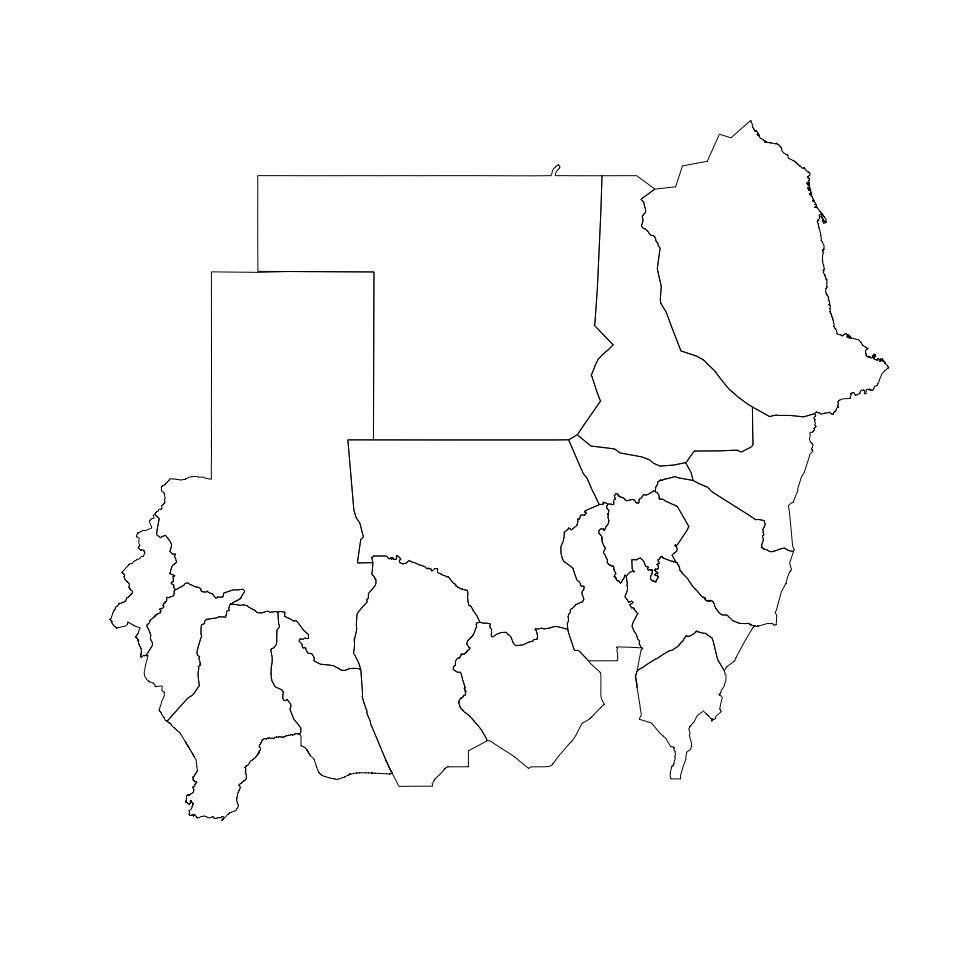
\includegraphics{figures/map1-1} 

}

\caption{Map of the states of Sudan with default plotting options}\label{fig:map1}
\end{figure}

~

From this plot of \texttt{sudan01} \texttt{SpatialPolygonsDataFrame}
object, we learn about some of the default plotting parameters under the
\texttt{sp} package. \emph{Line type} (\texttt{lty}) is set as a solid
line (\texttt{lty\ =\ 1}) and \emph{line width} (\texttt{lwd}) is set at
\texttt{lwd\ =\ 1}. \emph{Border colour} (\texttt{border}) is set as
\texttt{border\ =\ black} while the \emph{fill colour} (\texttt{col}) is
set at \texttt{col\ =\ NA}. We should remember that the class of
\texttt{sudan01} object is a \texttt{SpatialPolygonsDataFrame} hence it
is composed of closed rings that are not holes (i.e.~empty). Hence, in
the plotting parameters, border and fill colours are specified
separately.

Let us now try to plot another map of \texttt{sudan01} object but this
time change some of the default plotting parameters.

~

\begin{Shaded}
\begin{Highlighting}[]
\KeywordTok{plot}\NormalTok{(sudan01, }\DataTypeTok{lty =} \DecValTok{1}\NormalTok{, }\DataTypeTok{lwd =} \DecValTok{2}\NormalTok{, }\DataTypeTok{border =} \StringTok{"blue"}\NormalTok{, }\DataTypeTok{col =} \StringTok{"gray90"}\NormalTok{)}
\end{Highlighting}
\end{Shaded}

~

This command gives us the following map of Sudan:

~

\begin{figure}[H]

{\centering 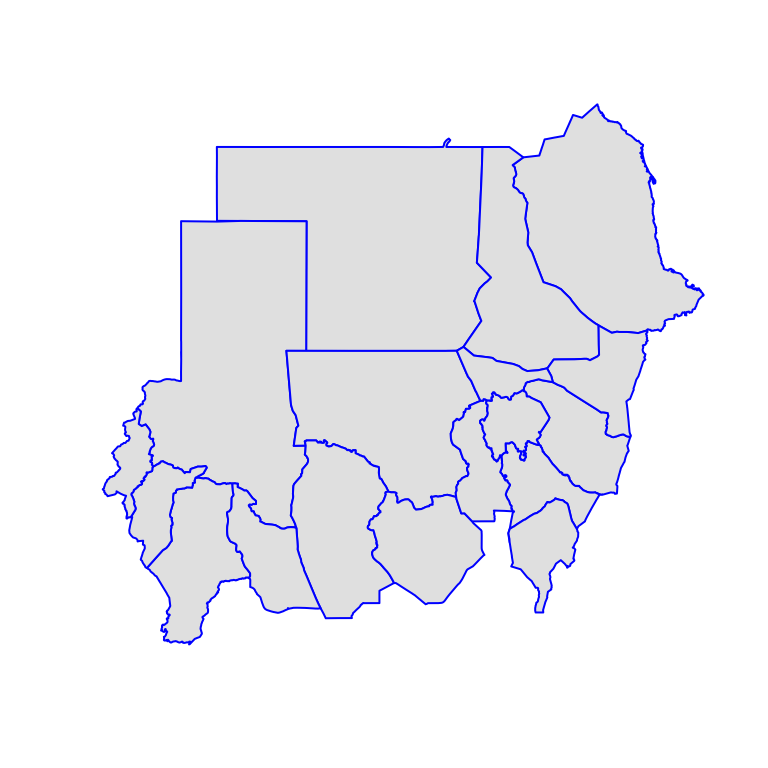
\includegraphics{figures/map2-1} 

}

\caption{Map of the states of Sudan with new plotting parameters}\label{fig:map2}
\end{figure}

~

The map above illustrates the changes in the plot created by the changes
in the plotting parameters that we have specified. The width of the
border is now thicker and its colour is now blue. The inside of the map
is now coloured gray.

So far we have focused a lot on \texttt{sudan01} object. Hence we have
learned a lot about the features, structure and characteristics of a
\textbf{polygon} and a \texttt{SpatialPolygonsDataFrame} that contains
\textbf{polygons} of each of the states of Sudan. However, we have yet
to work with another \texttt{SpatialPolygonsDataFrame} object named
\texttt{sudan02} which is a collection of \textbf{polygons} for each of
the localities in Sudan.

What we will try to learn now is how to work with the \texttt{sudan01}
and \texttt{sudan02} objects to create a map of Sudan that shows the
different localities and also shows how these localities are grouped in
order to make up each of the states in Sudan.

To be able to complete this task, we need to learn about \emph{map
layers}.

The idea of \emph{map layers} is that different set of map features
(i.e.~roads, topography, watery systems) that usually have separate
\textbf{shapefile} datasets are put together in a single map by plotting
each of these features on top of each other in layers. Depending on the
type and class of the \textbf{shapefile} objects being layered, the
order by which a feature is layered on to another determines which
features of which layer is visible or given emphasis.

Let us now try to layer \texttt{sudan01} and \texttt{sudan02} objects
such that the base map is that of the localities and on top is that of
the state boundaries. The final map will then show divisions by state
and then further subdivisions per state by localities. We call the
following commands to produce the map below:

~

\begin{Shaded}
\begin{Highlighting}[]
\CommentTok{#}
\CommentTok{# Plot localities of Sudan}
\CommentTok{#}
\KeywordTok{plot}\NormalTok{(sudan02, }\DataTypeTok{border =} \StringTok{"gray"}\NormalTok{)}
\CommentTok{#}
\CommentTok{# Plot states of Sudan}
\CommentTok{#}
\KeywordTok{plot}\NormalTok{(sudan01, }\DataTypeTok{lwd =} \DecValTok{2}\NormalTok{, }\DataTypeTok{add =} \OtherTok{TRUE}\NormalTok{)}
\end{Highlighting}
\end{Shaded}

\newpage

This produces the following map.

~

\begin{figure}[H]

{\centering 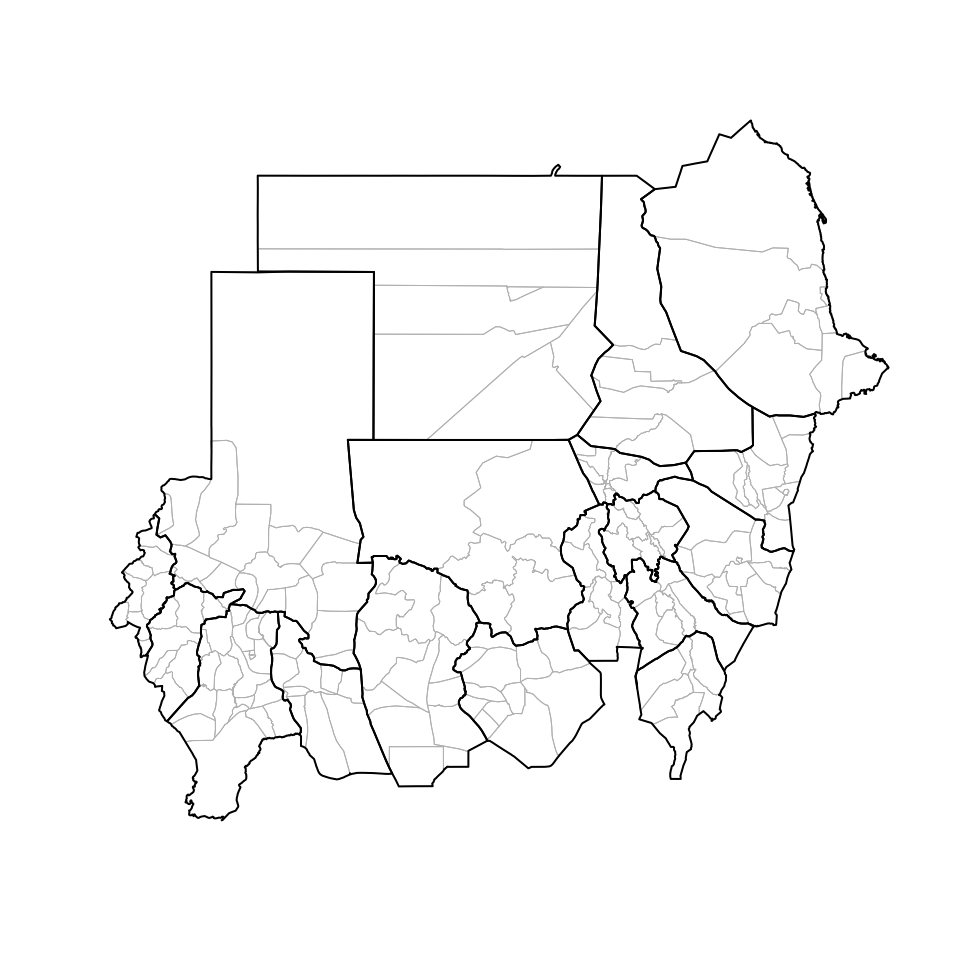
\includegraphics{figures/map3-1} 

}

\caption{Map of localities and states of Sudan}\label{fig:map3}
\end{figure}

~

Now, let us learn how to add layers of other \textbf{shapefile}
types/classes onto the base Sudan maps.

Earlier in Exercise \ref{exercise1}, we have retrieved the dataset for
the grid used in the Sudan S3M I and assigned it to the object
\texttt{grid12poly} and \texttt{grid12kmSudan}. The difference between
these two objects is that the first one is a
\texttt{SpatialPolygonsDataFrame} while the second is a
\texttt{SpatialLinesDataFrame}.

We will focus our attention to \texttt{grid12kmSudan} to familiarise
ourselves with the \texttt{SpatialLinesDataFrame} class objects. Let us
look at the structure of a \texttt{SpatialLinesDataFrame}.

~

\begin{Shaded}
\begin{Highlighting}[]
\KeywordTok{str}\NormalTok{(grid12kmSudan)}
\end{Highlighting}
\end{Shaded}

~

The results of this command is as expected quite long. But looking at
the first line of the output, we learn that \texttt{grid12kmSudan} has 4
slots.

~

\begin{verbatim}
#> Formal class 'SpatialLinesDataFrame' [package "sp"] with 4 slots
#>   ..@ data       :'data.frame':  245 obs. of  2 variables:
#>   .. ..$ ID   : chr [1:245] "0" "1" "2" "3" ...
#>   .. ..$ COORD: num [1:245] 23.1 23 23 22.9 22.8 ...
#>   ..@ lines      :List of 245
#>   .. ..$ :Formal class 'Lines' [package "sp"] with 2 slots
#>   .. .. .. ..@ Lines:List of 1
#>   .. .. .. .. ..$ :Formal class 'Line' [package "sp"] with 1 slot
#>   .. .. .. .. .. .. ..@ coords: num [1:2, 1:2] 21.8 38.6 23.1 23.1
#>   .. .. .. ..@ ID   : chr "0"
#>   .. ..$ :Formal class 'Lines' [package "sp"] with 2 slots
#>   .. .. .. ..@ Lines:List of 1
#>   .. .. .. .. ..$ :Formal class 'Line' [package "sp"] with 1 slot
#>   .. .. .. .. .. .. ..@ coords: num [1:2, 1:2] 21.8 38.6 23 23
#>   .. .. .. ..@ ID   : chr "1"
#>   .. ..$ :Formal class 'Lines' [package "sp"] with 2 slots
#>   .. .. .. ..@ Lines:List of 1
#>   .. .. .. .. ..$ :Formal class 'Line' [package "sp"] with 1 slot
#>   .. .. .. .. .. .. ..@ coords: num [1:2, 1:2] 21.8 38.6 23 23
#>   .. .. .. ..@ ID   : chr "2"
#>   .. ..$ :Formal class 'Lines' [package "sp"] with 2 slots
#>   .. .. .. ..@ Lines:List of 1
#>   .. .. .. .. ..$ :Formal class 'Line' [package "sp"] with 1 slot
#>   .. .. .. .. .. .. ..@ coords: num [1:2, 1:2] 21.8 38.6 22.9 22.9
#>   .. .. .. ..@ ID   : chr "3"
#>   .. ..$ :Formal class 'Lines' [package "sp"] with 2 slots
#>   .. .. .. ..@ Lines:List of 1
#>   .. .. .. .. ..$ :Formal class 'Line' [package "sp"] with 1 slot
#>   .. .. .. .. .. .. ..@ coords: num [1:2, 1:2] 21.8 38.6 22.8 22.8
#>   .. .. .. ..@ ID   : chr "4"
#>   .. ..$ :Formal class 'Lines' [package "sp"] with 2 slots
#>   .. .. .. ..@ Lines:List of 1
#>   .. .. .. .. ..$ :Formal class 'Line' [package "sp"] with 1 slot
#>   .. .. .. .. .. .. ..@ coords: num [1:2, 1:2] 21.8 38.6 22.7 22.7
#>   .. .. .. ..@ ID   : chr "5"
#>   .. ..$ :Formal class 'Lines' [package "sp"] with 2 slots
#>   .. .. .. ..@ Lines:List of 1
#>   .. .. .. .. ..$ :Formal class 'Line' [package "sp"] with 1 slot
#>   .. .. .. .. .. .. ..@ coords: num [1:2, 1:2] 21.8 38.6 22.6 22.6
#>   .. .. .. ..@ ID   : chr "6"
#>   .. ..$ :Formal class 'Lines' [package "sp"] with 2 slots
#>   .. .. .. ..@ Lines:List of 1
#>   .. .. .. .. ..$ :Formal class 'Line' [package "sp"] with 1 slot
#>   .. .. .. .. .. .. ..@ coords: num [1:2, 1:2] 21.8 38.6 22.5 22.5
#>   .. .. .. ..@ ID   : chr "7"
#>   .. ..$ :Formal class 'Lines' [package "sp"] with 2 slots
#>   .. .. .. ..@ Lines:List of 1
#>   .. .. .. .. ..$ :Formal class 'Line' [package "sp"] with 1 slot
#>   .. .. .. .. .. .. ..@ coords: num [1:2, 1:2] 21.8 38.6 22.4 22.4
#>   .. .. .. ..@ ID   : chr "8"
#>   .. ..$ :Formal class 'Lines' [package "sp"] with 2 slots
#>   .. .. .. ..@ Lines:List of 1
#>   .. .. .. .. ..$ :Formal class 'Line' [package "sp"] with 1 slot
#>   .. .. .. .. .. .. ..@ coords: num [1:2, 1:2] 21.8 38.6 22.3 22.3
#>   .. .. .. ..@ ID   : chr "9"
#>   .. ..$ :Formal class 'Lines' [package "sp"] with 2 slots
#>   .. .. .. ..@ Lines:List of 1
#>   .. .. .. .. ..$ :Formal class 'Line' [package "sp"] with 1 slot
#>   .. .. .. .. .. .. ..@ coords: num [1:2, 1:2] 21.8 38.6 22.2 22.2
#>   .. .. .. ..@ ID   : chr "10"
#>   .. ..$ :Formal class 'Lines' [package "sp"] with 2 slots
#>   .. .. .. ..@ Lines:List of 1
#>   .. .. .. .. ..$ :Formal class 'Line' [package "sp"] with 1 slot
#>   .. .. .. .. .. .. ..@ coords: num [1:2, 1:2] 21.8 38.6 22.1 22.1
#>   .. .. .. ..@ ID   : chr "11"
#>   .. ..$ :Formal class 'Lines' [package "sp"] with 2 slots
#>   .. .. .. ..@ Lines:List of 1
#>   .. .. .. .. ..$ :Formal class 'Line' [package "sp"] with 1 slot
#>   .. .. .. .. .. .. ..@ coords: num [1:2, 1:2] 21.8 38.6 22 22
#>   .. .. .. ..@ ID   : chr "12"
#>   .. ..$ :Formal class 'Lines' [package "sp"] with 2 slots
#>   .. .. .. ..@ Lines:List of 1
#>   .. .. .. .. ..$ :Formal class 'Line' [package "sp"] with 1 slot
#>   .. .. .. .. .. .. ..@ coords: num [1:2, 1:2] 21.8 38.6 21.9 21.9
#>   .. .. .. ..@ ID   : chr "13"
#>   .. ..$ :Formal class 'Lines' [package "sp"] with 2 slots
#>   .. .. .. ..@ Lines:List of 1
#>   .. .. .. .. ..$ :Formal class 'Line' [package "sp"] with 1 slot
#>   .. .. .. .. .. .. ..@ coords: num [1:2, 1:2] 21.8 38.6 21.8 21.8
#>   .. .. .. ..@ ID   : chr "14"
#>   .. ..$ :Formal class 'Lines' [package "sp"] with 2 slots
#>   .. .. .. ..@ Lines:List of 1
#>   .. .. .. .. ..$ :Formal class 'Line' [package "sp"] with 1 slot
#>   .. .. .. .. .. .. ..@ coords: num [1:2, 1:2] 21.8 38.6 21.7 21.7
#>   .. .. .. ..@ ID   : chr "15"
#>   .. ..$ :Formal class 'Lines' [package "sp"] with 2 slots
#>   .. .. .. ..@ Lines:List of 1
#>   .. .. .. .. ..$ :Formal class 'Line' [package "sp"] with 1 slot
#>   .. .. .. .. .. .. ..@ coords: num [1:2, 1:2] 21.8 38.6 21.6 21.6
#>   .. .. .. ..@ ID   : chr "16"
#>   .. ..$ :Formal class 'Lines' [package "sp"] with 2 slots
#>   .. .. .. ..@ Lines:List of 1
#>   .. .. .. .. ..$ :Formal class 'Line' [package "sp"] with 1 slot
#>   .. .. .. .. .. .. ..@ coords: num [1:2, 1:2] 21.8 38.6 21.5 21.5
#>   .. .. .. ..@ ID   : chr "17"
#>   .. ..$ :Formal class 'Lines' [package "sp"] with 2 slots
#>   .. .. .. ..@ Lines:List of 1
#>   .. .. .. .. ..$ :Formal class 'Line' [package "sp"] with 1 slot
#>   .. .. .. .. .. .. ..@ coords: num [1:2, 1:2] 21.8 38.6 21.4 21.4
#>   .. .. .. ..@ ID   : chr "18"
#>   .. ..$ :Formal class 'Lines' [package "sp"] with 2 slots
#>   .. .. .. ..@ Lines:List of 1
#>   .. .. .. .. ..$ :Formal class 'Line' [package "sp"] with 1 slot
#>   .. .. .. .. .. .. ..@ coords: num [1:2, 1:2] 21.8 38.6 21.4 21.4
#>   .. .. .. ..@ ID   : chr "19"
#>   .. ..$ :Formal class 'Lines' [package "sp"] with 2 slots
#>   .. .. .. ..@ Lines:List of 1
#>   .. .. .. .. ..$ :Formal class 'Line' [package "sp"] with 1 slot
#>   .. .. .. .. .. .. ..@ coords: num [1:2, 1:2] 21.8 38.6 21.3 21.3
#>   .. .. .. ..@ ID   : chr "20"
#>   .. ..$ :Formal class 'Lines' [package "sp"] with 2 slots
#>   .. .. .. ..@ Lines:List of 1
#>   .. .. .. .. ..$ :Formal class 'Line' [package "sp"] with 1 slot
#>   .. .. .. .. .. .. ..@ coords: num [1:2, 1:2] 21.8 38.6 21.2 21.2
#>   .. .. .. ..@ ID   : chr "21"
#>   .. ..$ :Formal class 'Lines' [package "sp"] with 2 slots
#>   .. .. .. ..@ Lines:List of 1
#>   .. .. .. .. ..$ :Formal class 'Line' [package "sp"] with 1 slot
#>   .. .. .. .. .. .. ..@ coords: num [1:2, 1:2] 21.8 38.6 21.1 21.1
#>   .. .. .. ..@ ID   : chr "22"
#>   .. ..$ :Formal class 'Lines' [package "sp"] with 2 slots
#>   .. .. .. ..@ Lines:List of 1
#>   .. .. .. .. ..$ :Formal class 'Line' [package "sp"] with 1 slot
#>   .. .. .. .. .. .. ..@ coords: num [1:2, 1:2] 21.8 38.6 21 21
#>   .. .. .. ..@ ID   : chr "23"
#>   .. ..$ :Formal class 'Lines' [package "sp"] with 2 slots
#>   .. .. .. ..@ Lines:List of 1
#>   .. .. .. .. ..$ :Formal class 'Line' [package "sp"] with 1 slot
#>   .. .. .. .. .. .. ..@ coords: num [1:2, 1:2] 21.8 38.6 20.9 20.9
#>   .. .. .. ..@ ID   : chr "24"
#>   .. ..$ :Formal class 'Lines' [package "sp"] with 2 slots
#>   .. .. .. ..@ Lines:List of 1
#>   .. .. .. .. ..$ :Formal class 'Line' [package "sp"] with 1 slot
#>   .. .. .. .. .. .. ..@ coords: num [1:2, 1:2] 21.8 38.6 20.8 20.8
#>   .. .. .. ..@ ID   : chr "25"
#>   .. ..$ :Formal class 'Lines' [package "sp"] with 2 slots
#>   .. .. .. ..@ Lines:List of 1
#>   .. .. .. .. ..$ :Formal class 'Line' [package "sp"] with 1 slot
#>   .. .. .. .. .. .. ..@ coords: num [1:2, 1:2] 21.8 38.6 20.7 20.7
#>   .. .. .. ..@ ID   : chr "26"
#>   .. ..$ :Formal class 'Lines' [package "sp"] with 2 slots
#>   .. .. .. ..@ Lines:List of 1
#>   .. .. .. .. ..$ :Formal class 'Line' [package "sp"] with 1 slot
#>   .. .. .. .. .. .. ..@ coords: num [1:2, 1:2] 21.8 38.6 20.6 20.6
#>   .. .. .. ..@ ID   : chr "27"
#>   .. ..$ :Formal class 'Lines' [package "sp"] with 2 slots
#>   .. .. .. ..@ Lines:List of 1
#>   .. .. .. .. ..$ :Formal class 'Line' [package "sp"] with 1 slot
#>   .. .. .. .. .. .. ..@ coords: num [1:2, 1:2] 21.8 38.6 20.5 20.5
#>   .. .. .. ..@ ID   : chr "28"
#>   .. ..$ :Formal class 'Lines' [package "sp"] with 2 slots
#>   .. .. .. ..@ Lines:List of 1
#>   .. .. .. .. ..$ :Formal class 'Line' [package "sp"] with 1 slot
#>   .. .. .. .. .. .. ..@ coords: num [1:2, 1:2] 21.8 38.6 20.4 20.4
#>   .. .. .. ..@ ID   : chr "29"
#>   .. ..$ :Formal class 'Lines' [package "sp"] with 2 slots
#>   .. .. .. ..@ Lines:List of 1
#>   .. .. .. .. ..$ :Formal class 'Line' [package "sp"] with 1 slot
#>   .. .. .. .. .. .. ..@ coords: num [1:2, 1:2] 21.8 38.6 20.3 20.3
#>   .. .. .. ..@ ID   : chr "30"
#>   .. ..$ :Formal class 'Lines' [package "sp"] with 2 slots
#>   .. .. .. ..@ Lines:List of 1
#>   .. .. .. .. ..$ :Formal class 'Line' [package "sp"] with 1 slot
#>   .. .. .. .. .. .. ..@ coords: num [1:2, 1:2] 21.8 38.6 20.2 20.2
#>   .. .. .. ..@ ID   : chr "31"
#>   .. ..$ :Formal class 'Lines' [package "sp"] with 2 slots
#>   .. .. .. ..@ Lines:List of 1
#>   .. .. .. .. ..$ :Formal class 'Line' [package "sp"] with 1 slot
#>   .. .. .. .. .. .. ..@ coords: num [1:2, 1:2] 21.8 38.6 20.1 20.1
#>   .. .. .. ..@ ID   : chr "32"
#>   .. ..$ :Formal class 'Lines' [package "sp"] with 2 slots
#>   .. .. .. ..@ Lines:List of 1
#>   .. .. .. .. ..$ :Formal class 'Line' [package "sp"] with 1 slot
#>   .. .. .. .. .. .. ..@ coords: num [1:2, 1:2] 21.8 38.6 20 20
#>   .. .. .. ..@ ID   : chr "33"
#>   .. ..$ :Formal class 'Lines' [package "sp"] with 2 slots
#>   .. .. .. ..@ Lines:List of 1
#>   .. .. .. .. ..$ :Formal class 'Line' [package "sp"] with 1 slot
#>   .. .. .. .. .. .. ..@ coords: num [1:2, 1:2] 21.8 38.6 19.9 19.9
#>   .. .. .. ..@ ID   : chr "34"
#>   .. ..$ :Formal class 'Lines' [package "sp"] with 2 slots
#>   .. .. .. ..@ Lines:List of 1
#>   .. .. .. .. ..$ :Formal class 'Line' [package "sp"] with 1 slot
#>   .. .. .. .. .. .. ..@ coords: num [1:2, 1:2] 21.8 38.6 19.9 19.9
#>   .. .. .. ..@ ID   : chr "35"
#>   .. ..$ :Formal class 'Lines' [package "sp"] with 2 slots
#>   .. .. .. ..@ Lines:List of 1
#>   .. .. .. .. ..$ :Formal class 'Line' [package "sp"] with 1 slot
#>   .. .. .. .. .. .. ..@ coords: num [1:2, 1:2] 21.8 38.6 19.8 19.8
#>   .. .. .. ..@ ID   : chr "36"
#>   .. ..$ :Formal class 'Lines' [package "sp"] with 2 slots
#>   .. .. .. ..@ Lines:List of 1
#>   .. .. .. .. ..$ :Formal class 'Line' [package "sp"] with 1 slot
#>   .. .. .. .. .. .. ..@ coords: num [1:2, 1:2] 21.8 38.6 19.7 19.7
#>   .. .. .. ..@ ID   : chr "37"
#>   .. ..$ :Formal class 'Lines' [package "sp"] with 2 slots
#>   .. .. .. ..@ Lines:List of 1
#>   .. .. .. .. ..$ :Formal class 'Line' [package "sp"] with 1 slot
#>   .. .. .. .. .. .. ..@ coords: num [1:2, 1:2] 21.8 38.6 19.6 19.6
#>   .. .. .. ..@ ID   : chr "38"
#>   .. ..$ :Formal class 'Lines' [package "sp"] with 2 slots
#>   .. .. .. ..@ Lines:List of 1
#>   .. .. .. .. ..$ :Formal class 'Line' [package "sp"] with 1 slot
#>   .. .. .. .. .. .. ..@ coords: num [1:2, 1:2] 21.8 38.6 19.5 19.5
#>   .. .. .. ..@ ID   : chr "39"
#>   .. ..$ :Formal class 'Lines' [package "sp"] with 2 slots
#>   .. .. .. ..@ Lines:List of 1
#>   .. .. .. .. ..$ :Formal class 'Line' [package "sp"] with 1 slot
#>   .. .. .. .. .. .. ..@ coords: num [1:2, 1:2] 21.8 38.6 19.4 19.4
#>   .. .. .. ..@ ID   : chr "40"
#>   .. ..$ :Formal class 'Lines' [package "sp"] with 2 slots
#>   .. .. .. ..@ Lines:List of 1
#>   .. .. .. .. ..$ :Formal class 'Line' [package "sp"] with 1 slot
#>   .. .. .. .. .. .. ..@ coords: num [1:2, 1:2] 21.8 38.6 19.3 19.3
#>   .. .. .. ..@ ID   : chr "41"
#>   .. ..$ :Formal class 'Lines' [package "sp"] with 2 slots
#>   .. .. .. ..@ Lines:List of 1
#>   .. .. .. .. ..$ :Formal class 'Line' [package "sp"] with 1 slot
#>   .. .. .. .. .. .. ..@ coords: num [1:2, 1:2] 21.8 38.6 19.2 19.2
#>   .. .. .. ..@ ID   : chr "42"
#>   .. ..$ :Formal class 'Lines' [package "sp"] with 2 slots
#>   .. .. .. ..@ Lines:List of 1
#>   .. .. .. .. ..$ :Formal class 'Line' [package "sp"] with 1 slot
#>   .. .. .. .. .. .. ..@ coords: num [1:2, 1:2] 21.8 38.6 19.1 19.1
#>   .. .. .. ..@ ID   : chr "43"
#>   .. ..$ :Formal class 'Lines' [package "sp"] with 2 slots
#>   .. .. .. ..@ Lines:List of 1
#>   .. .. .. .. ..$ :Formal class 'Line' [package "sp"] with 1 slot
#>   .. .. .. .. .. .. ..@ coords: num [1:2, 1:2] 21.8 38.6 19 19
#>   .. .. .. ..@ ID   : chr "44"
#>   .. ..$ :Formal class 'Lines' [package "sp"] with 2 slots
#>   .. .. .. ..@ Lines:List of 1
#>   .. .. .. .. ..$ :Formal class 'Line' [package "sp"] with 1 slot
#>   .. .. .. .. .. .. ..@ coords: num [1:2, 1:2] 21.8 38.6 18.9 18.9
#>   .. .. .. ..@ ID   : chr "45"
#>   .. ..$ :Formal class 'Lines' [package "sp"] with 2 slots
#>   .. .. .. ..@ Lines:List of 1
#>   .. .. .. .. ..$ :Formal class 'Line' [package "sp"] with 1 slot
#>   .. .. .. .. .. .. ..@ coords: num [1:2, 1:2] 21.8 38.6 18.8 18.8
#>   .. .. .. ..@ ID   : chr "46"
#>   .. ..$ :Formal class 'Lines' [package "sp"] with 2 slots
#>   .. .. .. ..@ Lines:List of 1
#>   .. .. .. .. ..$ :Formal class 'Line' [package "sp"] with 1 slot
#>   .. .. .. .. .. .. ..@ coords: num [1:2, 1:2] 21.8 38.6 18.7 18.7
#>   .. .. .. ..@ ID   : chr "47"
#>   .. ..$ :Formal class 'Lines' [package "sp"] with 2 slots
#>   .. .. .. ..@ Lines:List of 1
#>   .. .. .. .. ..$ :Formal class 'Line' [package "sp"] with 1 slot
#>   .. .. .. .. .. .. ..@ coords: num [1:2, 1:2] 21.8 38.6 18.6 18.6
#>   .. .. .. ..@ ID   : chr "48"
#>   .. ..$ :Formal class 'Lines' [package "sp"] with 2 slots
#>   .. .. .. ..@ Lines:List of 1
#>   .. .. .. .. ..$ :Formal class 'Line' [package "sp"] with 1 slot
#>   .. .. .. .. .. .. ..@ coords: num [1:2, 1:2] 21.8 38.6 18.5 18.5
#>   .. .. .. ..@ ID   : chr "49"
#>   .. ..$ :Formal class 'Lines' [package "sp"] with 2 slots
#>   .. .. .. ..@ Lines:List of 1
#>   .. .. .. .. ..$ :Formal class 'Line' [package "sp"] with 1 slot
#>   .. .. .. .. .. .. ..@ coords: num [1:2, 1:2] 21.8 38.6 18.4 18.4
#>   .. .. .. ..@ ID   : chr "50"
#>   .. ..$ :Formal class 'Lines' [package "sp"] with 2 slots
#>   .. .. .. ..@ Lines:List of 1
#>   .. .. .. .. ..$ :Formal class 'Line' [package "sp"] with 1 slot
#>   .. .. .. .. .. .. ..@ coords: num [1:2, 1:2] 21.8 38.6 18.3 18.3
#>   .. .. .. ..@ ID   : chr "51"
#>   .. ..$ :Formal class 'Lines' [package "sp"] with 2 slots
#>   .. .. .. ..@ Lines:List of 1
#>   .. .. .. .. ..$ :Formal class 'Line' [package "sp"] with 1 slot
#>   .. .. .. .. .. .. ..@ coords: num [1:2, 1:2] 21.8 38.6 18.3 18.3
#>   .. .. .. ..@ ID   : chr "52"
#>   .. ..$ :Formal class 'Lines' [package "sp"] with 2 slots
#>   .. .. .. ..@ Lines:List of 1
#>   .. .. .. .. ..$ :Formal class 'Line' [package "sp"] with 1 slot
#>   .. .. .. .. .. .. ..@ coords: num [1:2, 1:2] 21.8 38.6 18.2 18.2
#>   .. .. .. ..@ ID   : chr "53"
#>   .. ..$ :Formal class 'Lines' [package "sp"] with 2 slots
#>   .. .. .. ..@ Lines:List of 1
#>   .. .. .. .. ..$ :Formal class 'Line' [package "sp"] with 1 slot
#>   .. .. .. .. .. .. ..@ coords: num [1:2, 1:2] 21.8 38.6 18.1 18.1
#>   .. .. .. ..@ ID   : chr "54"
#>   .. ..$ :Formal class 'Lines' [package "sp"] with 2 slots
#>   .. .. .. ..@ Lines:List of 1
#>   .. .. .. .. ..$ :Formal class 'Line' [package "sp"] with 1 slot
#>   .. .. .. .. .. .. ..@ coords: num [1:2, 1:2] 21.8 38.6 18 18
#>   .. .. .. ..@ ID   : chr "55"
#>   .. ..$ :Formal class 'Lines' [package "sp"] with 2 slots
#>   .. .. .. ..@ Lines:List of 1
#>   .. .. .. .. ..$ :Formal class 'Line' [package "sp"] with 1 slot
#>   .. .. .. .. .. .. ..@ coords: num [1:2, 1:2] 21.8 38.6 17.9 17.9
#>   .. .. .. ..@ ID   : chr "56"
#>   .. ..$ :Formal class 'Lines' [package "sp"] with 2 slots
#>   .. .. .. ..@ Lines:List of 1
#>   .. .. .. .. ..$ :Formal class 'Line' [package "sp"] with 1 slot
#>   .. .. .. .. .. .. ..@ coords: num [1:2, 1:2] 21.8 38.6 17.8 17.8
#>   .. .. .. ..@ ID   : chr "57"
#>   .. ..$ :Formal class 'Lines' [package "sp"] with 2 slots
#>   .. .. .. ..@ Lines:List of 1
#>   .. .. .. .. ..$ :Formal class 'Line' [package "sp"] with 1 slot
#>   .. .. .. .. .. .. ..@ coords: num [1:2, 1:2] 21.8 38.6 17.7 17.7
#>   .. .. .. ..@ ID   : chr "58"
#>   .. ..$ :Formal class 'Lines' [package "sp"] with 2 slots
#>   .. .. .. ..@ Lines:List of 1
#>   .. .. .. .. ..$ :Formal class 'Line' [package "sp"] with 1 slot
#>   .. .. .. .. .. .. ..@ coords: num [1:2, 1:2] 21.8 38.6 17.6 17.6
#>   .. .. .. ..@ ID   : chr "59"
#>   .. ..$ :Formal class 'Lines' [package "sp"] with 2 slots
#>   .. .. .. ..@ Lines:List of 1
#>   .. .. .. .. ..$ :Formal class 'Line' [package "sp"] with 1 slot
#>   .. .. .. .. .. .. ..@ coords: num [1:2, 1:2] 21.8 38.6 17.5 17.5
#>   .. .. .. ..@ ID   : chr "60"
#>   .. ..$ :Formal class 'Lines' [package "sp"] with 2 slots
#>   .. .. .. ..@ Lines:List of 1
#>   .. .. .. .. ..$ :Formal class 'Line' [package "sp"] with 1 slot
#>   .. .. .. .. .. .. ..@ coords: num [1:2, 1:2] 21.8 38.6 17.4 17.4
#>   .. .. .. ..@ ID   : chr "61"
#>   .. ..$ :Formal class 'Lines' [package "sp"] with 2 slots
#>   .. .. .. ..@ Lines:List of 1
#>   .. .. .. .. ..$ :Formal class 'Line' [package "sp"] with 1 slot
#>   .. .. .. .. .. .. ..@ coords: num [1:2, 1:2] 21.8 38.6 17.3 17.3
#>   .. .. .. ..@ ID   : chr "62"
#>   .. ..$ :Formal class 'Lines' [package "sp"] with 2 slots
#>   .. .. .. ..@ Lines:List of 1
#>   .. .. .. .. ..$ :Formal class 'Line' [package "sp"] with 1 slot
#>   .. .. .. .. .. .. ..@ coords: num [1:2, 1:2] 21.8 38.6 17.2 17.2
#>   .. .. .. ..@ ID   : chr "63"
#>   .. ..$ :Formal class 'Lines' [package "sp"] with 2 slots
#>   .. .. .. ..@ Lines:List of 1
#>   .. .. .. .. ..$ :Formal class 'Line' [package "sp"] with 1 slot
#>   .. .. .. .. .. .. ..@ coords: num [1:2, 1:2] 21.8 38.6 17.1 17.1
#>   .. .. .. ..@ ID   : chr "64"
#>   .. ..$ :Formal class 'Lines' [package "sp"] with 2 slots
#>   .. .. .. ..@ Lines:List of 1
#>   .. .. .. .. ..$ :Formal class 'Line' [package "sp"] with 1 slot
#>   .. .. .. .. .. .. ..@ coords: num [1:2, 1:2] 21.8 38.6 17 17
#>   .. .. .. ..@ ID   : chr "65"
#>   .. ..$ :Formal class 'Lines' [package "sp"] with 2 slots
#>   .. .. .. ..@ Lines:List of 1
#>   .. .. .. .. ..$ :Formal class 'Line' [package "sp"] with 1 slot
#>   .. .. .. .. .. .. ..@ coords: num [1:2, 1:2] 21.8 38.6 16.9 16.9
#>   .. .. .. ..@ ID   : chr "66"
#>   .. ..$ :Formal class 'Lines' [package "sp"] with 2 slots
#>   .. .. .. ..@ Lines:List of 1
#>   .. .. .. .. ..$ :Formal class 'Line' [package "sp"] with 1 slot
#>   .. .. .. .. .. .. ..@ coords: num [1:2, 1:2] 21.8 38.6 16.8 16.8
#>   .. .. .. ..@ ID   : chr "67"
#>   .. ..$ :Formal class 'Lines' [package "sp"] with 2 slots
#>   .. .. .. ..@ Lines:List of 1
#>   .. .. .. .. ..$ :Formal class 'Line' [package "sp"] with 1 slot
#>   .. .. .. .. .. .. ..@ coords: num [1:2, 1:2] 21.8 38.6 16.7 16.7
#>   .. .. .. ..@ ID   : chr "68"
#>   .. ..$ :Formal class 'Lines' [package "sp"] with 2 slots
#>   .. .. .. ..@ Lines:List of 1
#>   .. .. .. .. ..$ :Formal class 'Line' [package "sp"] with 1 slot
#>   .. .. .. .. .. .. ..@ coords: num [1:2, 1:2] 21.8 38.6 16.7 16.7
#>   .. .. .. ..@ ID   : chr "69"
#>   .. ..$ :Formal class 'Lines' [package "sp"] with 2 slots
#>   .. .. .. ..@ Lines:List of 1
#>   .. .. .. .. ..$ :Formal class 'Line' [package "sp"] with 1 slot
#>   .. .. .. .. .. .. ..@ coords: num [1:2, 1:2] 21.8 38.6 16.6 16.6
#>   .. .. .. ..@ ID   : chr "70"
#>   .. ..$ :Formal class 'Lines' [package "sp"] with 2 slots
#>   .. .. .. ..@ Lines:List of 1
#>   .. .. .. .. ..$ :Formal class 'Line' [package "sp"] with 1 slot
#>   .. .. .. .. .. .. ..@ coords: num [1:2, 1:2] 21.8 38.6 16.5 16.5
#>   .. .. .. ..@ ID   : chr "71"
#>   .. ..$ :Formal class 'Lines' [package "sp"] with 2 slots
#>   .. .. .. ..@ Lines:List of 1
#>   .. .. .. .. ..$ :Formal class 'Line' [package "sp"] with 1 slot
#>   .. .. .. .. .. .. ..@ coords: num [1:2, 1:2] 21.8 38.6 16.4 16.4
#>   .. .. .. ..@ ID   : chr "72"
#>   .. ..$ :Formal class 'Lines' [package "sp"] with 2 slots
#>   .. .. .. ..@ Lines:List of 1
#>   .. .. .. .. ..$ :Formal class 'Line' [package "sp"] with 1 slot
#>   .. .. .. .. .. .. ..@ coords: num [1:2, 1:2] 21.8 38.6 16.3 16.3
#>   .. .. .. ..@ ID   : chr "73"
#>   .. ..$ :Formal class 'Lines' [package "sp"] with 2 slots
#>   .. .. .. ..@ Lines:List of 1
#>   .. .. .. .. ..$ :Formal class 'Line' [package "sp"] with 1 slot
#>   .. .. .. .. .. .. ..@ coords: num [1:2, 1:2] 21.8 38.6 16.2 16.2
#>   .. .. .. ..@ ID   : chr "74"
#>   .. ..$ :Formal class 'Lines' [package "sp"] with 2 slots
#>   .. .. .. ..@ Lines:List of 1
#>   .. .. .. .. ..$ :Formal class 'Line' [package "sp"] with 1 slot
#>   .. .. .. .. .. .. ..@ coords: num [1:2, 1:2] 21.8 38.6 16.1 16.1
#>   .. .. .. ..@ ID   : chr "75"
#>   .. ..$ :Formal class 'Lines' [package "sp"] with 2 slots
#>   .. .. .. ..@ Lines:List of 1
#>   .. .. .. .. ..$ :Formal class 'Line' [package "sp"] with 1 slot
#>   .. .. .. .. .. .. ..@ coords: num [1:2, 1:2] 21.8 38.6 16 16
#>   .. .. .. ..@ ID   : chr "76"
#>   .. ..$ :Formal class 'Lines' [package "sp"] with 2 slots
#>   .. .. .. ..@ Lines:List of 1
#>   .. .. .. .. ..$ :Formal class 'Line' [package "sp"] with 1 slot
#>   .. .. .. .. .. .. ..@ coords: num [1:2, 1:2] 21.8 38.6 15.9 15.9
#>   .. .. .. ..@ ID   : chr "77"
#>   .. ..$ :Formal class 'Lines' [package "sp"] with 2 slots
#>   .. .. .. ..@ Lines:List of 1
#>   .. .. .. .. ..$ :Formal class 'Line' [package "sp"] with 1 slot
#>   .. .. .. .. .. .. ..@ coords: num [1:2, 1:2] 21.8 38.6 15.8 15.8
#>   .. .. .. ..@ ID   : chr "78"
#>   .. ..$ :Formal class 'Lines' [package "sp"] with 2 slots
#>   .. .. .. ..@ Lines:List of 1
#>   .. .. .. .. ..$ :Formal class 'Line' [package "sp"] with 1 slot
#>   .. .. .. .. .. .. ..@ coords: num [1:2, 1:2] 21.8 38.6 15.7 15.7
#>   .. .. .. ..@ ID   : chr "79"
#>   .. ..$ :Formal class 'Lines' [package "sp"] with 2 slots
#>   .. .. .. ..@ Lines:List of 1
#>   .. .. .. .. ..$ :Formal class 'Line' [package "sp"] with 1 slot
#>   .. .. .. .. .. .. ..@ coords: num [1:2, 1:2] 21.8 38.6 15.6 15.6
#>   .. .. .. ..@ ID   : chr "80"
#>   .. ..$ :Formal class 'Lines' [package "sp"] with 2 slots
#>   .. .. .. ..@ Lines:List of 1
#>   .. .. .. .. ..$ :Formal class 'Line' [package "sp"] with 1 slot
#>   .. .. .. .. .. .. ..@ coords: num [1:2, 1:2] 21.8 38.6 15.5 15.5
#>   .. .. .. ..@ ID   : chr "81"
#>   .. ..$ :Formal class 'Lines' [package "sp"] with 2 slots
#>   .. .. .. ..@ Lines:List of 1
#>   .. .. .. .. ..$ :Formal class 'Line' [package "sp"] with 1 slot
#>   .. .. .. .. .. .. ..@ coords: num [1:2, 1:2] 21.8 38.6 15.4 15.4
#>   .. .. .. ..@ ID   : chr "82"
#>   .. ..$ :Formal class 'Lines' [package "sp"] with 2 slots
#>   .. .. .. ..@ Lines:List of 1
#>   .. .. .. .. ..$ :Formal class 'Line' [package "sp"] with 1 slot
#>   .. .. .. .. .. .. ..@ coords: num [1:2, 1:2] 21.8 38.6 15.3 15.3
#>   .. .. .. ..@ ID   : chr "83"
#>   .. ..$ :Formal class 'Lines' [package "sp"] with 2 slots
#>   .. .. .. ..@ Lines:List of 1
#>   .. .. .. .. ..$ :Formal class 'Line' [package "sp"] with 1 slot
#>   .. .. .. .. .. .. ..@ coords: num [1:2, 1:2] 21.8 38.6 15.2 15.2
#>   .. .. .. ..@ ID   : chr "84"
#>   .. ..$ :Formal class 'Lines' [package "sp"] with 2 slots
#>   .. .. .. ..@ Lines:List of 1
#>   .. .. .. .. ..$ :Formal class 'Line' [package "sp"] with 1 slot
#>   .. .. .. .. .. .. ..@ coords: num [1:2, 1:2] 21.8 38.6 15.1 15.1
#>   .. .. .. ..@ ID   : chr "85"
#>   .. ..$ :Formal class 'Lines' [package "sp"] with 2 slots
#>   .. .. .. ..@ Lines:List of 1
#>   .. .. .. .. ..$ :Formal class 'Line' [package "sp"] with 1 slot
#>   .. .. .. .. .. .. ..@ coords: num [1:2, 1:2] 21.8 38.6 15.1 15.1
#>   .. .. .. ..@ ID   : chr "86"
#>   .. ..$ :Formal class 'Lines' [package "sp"] with 2 slots
#>   .. .. .. ..@ Lines:List of 1
#>   .. .. .. .. ..$ :Formal class 'Line' [package "sp"] with 1 slot
#>   .. .. .. .. .. .. ..@ coords: num [1:2, 1:2] 21.8 38.6 15 15
#>   .. .. .. ..@ ID   : chr "87"
#>   .. ..$ :Formal class 'Lines' [package "sp"] with 2 slots
#>   .. .. .. ..@ Lines:List of 1
#>   .. .. .. .. ..$ :Formal class 'Line' [package "sp"] with 1 slot
#>   .. .. .. .. .. .. ..@ coords: num [1:2, 1:2] 21.8 38.6 14.9 14.9
#>   .. .. .. ..@ ID   : chr "88"
#>   .. ..$ :Formal class 'Lines' [package "sp"] with 2 slots
#>   .. .. .. ..@ Lines:List of 1
#>   .. .. .. .. ..$ :Formal class 'Line' [package "sp"] with 1 slot
#>   .. .. .. .. .. .. ..@ coords: num [1:2, 1:2] 21.8 38.6 14.8 14.8
#>   .. .. .. ..@ ID   : chr "89"
#>   .. ..$ :Formal class 'Lines' [package "sp"] with 2 slots
#>   .. .. .. ..@ Lines:List of 1
#>   .. .. .. .. ..$ :Formal class 'Line' [package "sp"] with 1 slot
#>   .. .. .. .. .. .. ..@ coords: num [1:2, 1:2] 21.8 38.6 14.7 14.7
#>   .. .. .. ..@ ID   : chr "90"
#>   .. ..$ :Formal class 'Lines' [package "sp"] with 2 slots
#>   .. .. .. ..@ Lines:List of 1
#>   .. .. .. .. ..$ :Formal class 'Line' [package "sp"] with 1 slot
#>   .. .. .. .. .. .. ..@ coords: num [1:2, 1:2] 21.8 38.6 14.6 14.6
#>   .. .. .. ..@ ID   : chr "91"
#>   .. ..$ :Formal class 'Lines' [package "sp"] with 2 slots
#>   .. .. .. ..@ Lines:List of 1
#>   .. .. .. .. ..$ :Formal class 'Line' [package "sp"] with 1 slot
#>   .. .. .. .. .. .. ..@ coords: num [1:2, 1:2] 21.8 38.6 14.5 14.5
#>   .. .. .. ..@ ID   : chr "92"
#>   .. ..$ :Formal class 'Lines' [package "sp"] with 2 slots
#>   .. .. .. ..@ Lines:List of 1
#>   .. .. .. .. ..$ :Formal class 'Line' [package "sp"] with 1 slot
#>   .. .. .. .. .. .. ..@ coords: num [1:2, 1:2] 21.8 38.6 14.4 14.4
#>   .. .. .. ..@ ID   : chr "93"
#>   .. ..$ :Formal class 'Lines' [package "sp"] with 2 slots
#>   .. .. .. ..@ Lines:List of 1
#>   .. .. .. .. ..$ :Formal class 'Line' [package "sp"] with 1 slot
#>   .. .. .. .. .. .. ..@ coords: num [1:2, 1:2] 21.8 38.6 14.3 14.3
#>   .. .. .. ..@ ID   : chr "94"
#>   .. ..$ :Formal class 'Lines' [package "sp"] with 2 slots
#>   .. .. .. ..@ Lines:List of 1
#>   .. .. .. .. ..$ :Formal class 'Line' [package "sp"] with 1 slot
#>   .. .. .. .. .. .. ..@ coords: num [1:2, 1:2] 21.8 38.6 14.2 14.2
#>   .. .. .. ..@ ID   : chr "95"
#>   .. ..$ :Formal class 'Lines' [package "sp"] with 2 slots
#>   .. .. .. ..@ Lines:List of 1
#>   .. .. .. .. ..$ :Formal class 'Line' [package "sp"] with 1 slot
#>   .. .. .. .. .. .. ..@ coords: num [1:2, 1:2] 21.8 38.6 14.1 14.1
#>   .. .. .. ..@ ID   : chr "96"
#>   .. ..$ :Formal class 'Lines' [package "sp"] with 2 slots
#>   .. .. .. ..@ Lines:List of 1
#>   .. .. .. .. ..$ :Formal class 'Line' [package "sp"] with 1 slot
#>   .. .. .. .. .. .. ..@ coords: num [1:2, 1:2] 21.8 38.6 14 14
#>   .. .. .. ..@ ID   : chr "97"
#>   .. ..$ :Formal class 'Lines' [package "sp"] with 2 slots
#>   .. .. .. ..@ Lines:List of 1
#>   .. .. .. .. ..$ :Formal class 'Line' [package "sp"] with 1 slot
#>   .. .. .. .. .. .. ..@ coords: num [1:2, 1:2] 21.8 38.6 13.9 13.9
#>   .. .. .. ..@ ID   : chr "98"
#>   .. .. [list output truncated]
#>   ..@ bbox       : num [1:2, 1:2] 21.81 8.64 38.59 23.14
#>   .. ..- attr(*, "dimnames")=List of 2
#>   .. .. ..$ : chr [1:2] "x" "y"
#>   .. .. ..$ : chr [1:2] "min" "max"
#>   ..@ proj4string:Formal class 'CRS' [package "sp"] with 1 slot
#>   .. .. ..@ projargs: chr "+proj=longlat +datum=WGS84 +no_defs +ellps=WGS84 +towgs84=0,0,0"
\end{verbatim}

\newpage

The 4 slots in a \texttt{SpatialLinesDataFrame} are:

~

\begin{longtable}[]{@{}ll@{}}
\caption{\label{tab:table3} SpatialLinesDataFrame structure}\tabularnewline
\toprule
\begin{minipage}[t]{0.32\columnwidth}\raggedright
\textbf{data}\strut
\end{minipage} & \begin{minipage}[t]{0.62\columnwidth}\raggedright
Contains the index or reference data frame of the \textbf{shapefile} the
number of rows of which indicates the number of \emph{lines} that
comprise the entire \textbf{shapefile}\strut
\end{minipage}\tabularnewline
\begin{minipage}[t]{0.32\columnwidth}\raggedright
\textbf{lines}\strut
\end{minipage} & \begin{minipage}[t]{0.62\columnwidth}\raggedright
Contains \emph{n} number of datasets based on the number of \emph{lines}
that comprise the entire \textbf{shapefile}.\strut
\end{minipage}\tabularnewline
\begin{minipage}[t]{0.32\columnwidth}\raggedright
\textbf{bbox}\strut
\end{minipage} & \begin{minipage}[t]{0.62\columnwidth}\raggedright
Contains a matrix the values of which are the minimum and maximum
\texttt{x} and \texttt{y} limits of the entire \textbf{shapefile}.\strut
\end{minipage}\tabularnewline
\begin{minipage}[t]{0.32\columnwidth}\raggedright
\textbf{proj4string}\strut
\end{minipage} & \begin{minipage}[t]{0.62\columnwidth}\raggedright
Contains a character string that specifies the projection and datum of
the \textbf{shapefile} object\strut
\end{minipage}\tabularnewline
\bottomrule
\end{longtable}

~

Compared to the \texttt{SpatialPolygonsDataFrame},
\texttt{grid12kmSudan} has a slot for \emph{lines} (as expected) but
doesn't have the \texttt{plotOrder} slot. If we look back at what we've
learned regarding \texttt{plotOrder}, it is understandable why this is
not included in a \texttt{SpatialLinesDataFrame} object. The
\texttt{plotOrder} is determined by the area of the shapes in the
object. However, \texttt{SpatialLinesDataFrame} objects does not have a
value for area because it is just composed of \emph{lines}, not
\emph{polygons}.

A closer look at the slot \texttt{grid12kmSudan@lines}, we notice that
the data structure is much simpler than that of \emph{polygons}. Each
\emph{line} is simply defined by a set of 2 points.

Let us now add the \texttt{grid12kmSudan} object as another \emph{layer}
on our map. We should put it on top of \texttt{sudan02} and
\texttt{sudan01} with a thin \emph{line width} (\texttt{\textless{}\ 1})
and a light colour. Here is the command that will produce this.

~

\begin{Shaded}
\begin{Highlighting}[]
\KeywordTok{plot}\NormalTok{(sudan02, }\DataTypeTok{border =} \StringTok{"gray"}\NormalTok{)}
\KeywordTok{plot}\NormalTok{(sudan01, }\DataTypeTok{lwd =} \DecValTok{2}\NormalTok{, }\DataTypeTok{add =} \OtherTok{TRUE}\NormalTok{)}
\KeywordTok{plot}\NormalTok{(grid12kmSudan, }\DataTypeTok{lwd =} \FloatTok{0.5}\NormalTok{, }\DataTypeTok{col =} \StringTok{"gray90"}\NormalTok{, }\DataTypeTok{add =} \OtherTok{TRUE}\NormalTok{)}
\end{Highlighting}
\end{Shaded}

\newpage

This command produces the following map:

~

\begin{figure}[H]

{\centering 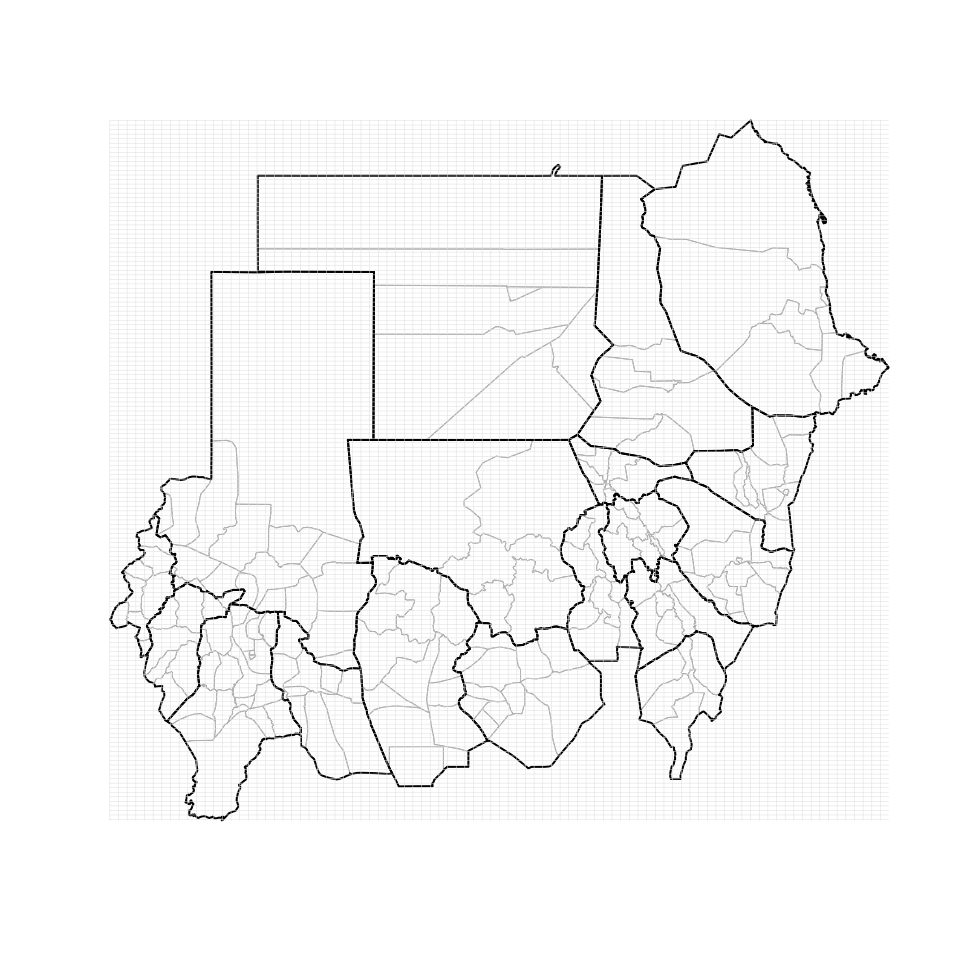
\includegraphics{figures/map4-1} 

}

\caption{Map of localities and states of Sudan with rectangular grid}\label{fig:map4}
\end{figure}

~

Now let us learn about points data.

Earlier, we have created an object called \texttt{villages}. This object
contains village data for the whole of Sudan with their \texttt{x} and
\texttt{y} geographical coordinates.

If we check the class of the object \texttt{villages}

~

\begin{Shaded}
\begin{Highlighting}[]
\KeywordTok{class}\NormalTok{(villages)}
\end{Highlighting}
\end{Shaded}

\newpage

we find out that this object is a data.frame and not an sp class object.

~

\begin{verbatim}
#> [1] "data.frame"
\end{verbatim}

~

However, this object is still map data because it contains geographic
information which in this case is the \texttt{x} and \texttt{y}
coordinates of the villages of Sudan.

This is the only information we need to be able to plot points data on
the map. We can do this by calling the following commands:

~

\begin{Shaded}
\begin{Highlighting}[]
\KeywordTok{plot}\NormalTok{(sudan02, }\DataTypeTok{border =} \StringTok{"gray"}\NormalTok{)}
\KeywordTok{plot}\NormalTok{(sudan01, }\DataTypeTok{lwd =} \DecValTok{2}\NormalTok{, }\DataTypeTok{add =} \OtherTok{TRUE}\NormalTok{)}
\KeywordTok{plot}\NormalTok{(grid12kmSudan, }\DataTypeTok{lwd =} \FloatTok{0.5}\NormalTok{, }\DataTypeTok{col =} \StringTok{"gray90"}\NormalTok{, }\DataTypeTok{add =} \OtherTok{TRUE}\NormalTok{)}
\KeywordTok{points}\NormalTok{(villages}\OperatorTok{$}\NormalTok{X, villages}\OperatorTok{$}\NormalTok{Y, }\DataTypeTok{pch =} \DecValTok{20}\NormalTok{, }\DataTypeTok{cex =} \FloatTok{0.2}\NormalTok{, }\DataTypeTok{col =} \StringTok{"gray90"}\NormalTok{)}
\end{Highlighting}
\end{Shaded}

\newpage

This produces the following map.

~

\begin{figure}[H]

{\centering 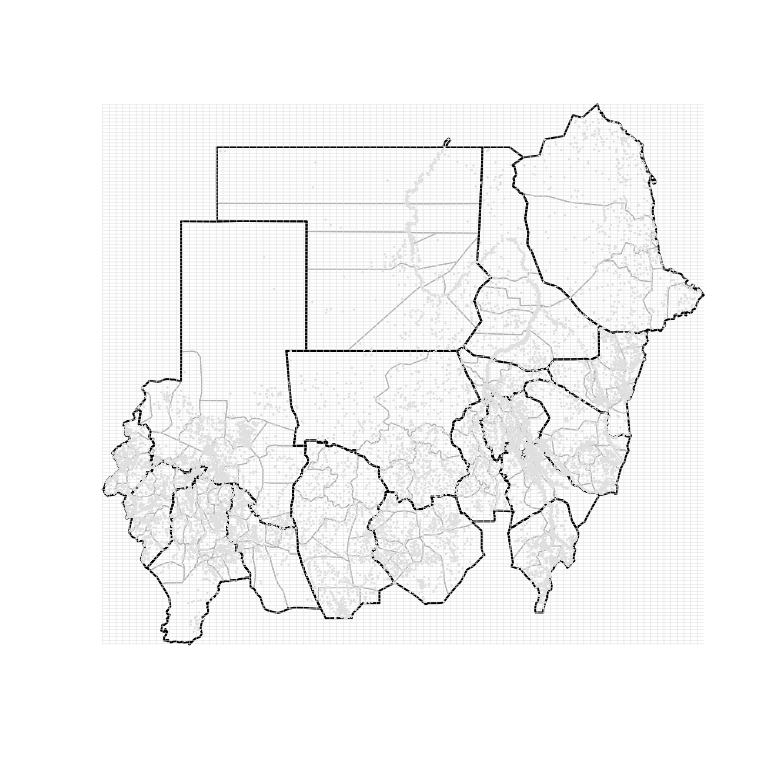
\includegraphics{figures/map5-1} 

}

\caption{Map of localities and states of Sudan with rectangular grid and villages}\label{fig:map5}
\end{figure}

~

In the commands above, we learn a new function called \texttt{points()}
and some new graphical parameters that are useful in plotting
\emph{points}.

The \texttt{points()} function basically instructs \textbf{R} to plot a
series of \emph{points} given the specified coordinates. The kind of
character that is drawn to represent the \emph{point} is determined by
the parameter called \texttt{pch} (\emph{point character}) with default
being a hollow circle.

\newpage

The most commonly used point characters are specified by the following
numeric values:

~

\begin{center}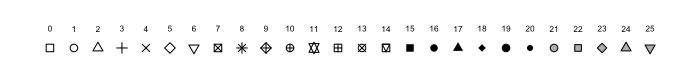
\includegraphics[width=0.9\linewidth]{figures/pch} \end{center}

~

In this case, we used \texttt{pch\ =\ 20} which is a solid point that is
2/3 the size of \texttt{pch\ =\ 19}.

The other graphical parameter that we learn here is \texttt{cex}
(\emph{character expansion}) which determines the size of the point
character and has a default value of \texttt{cex\ =\ 1}.

By now you would have noticed that when we used the \texttt{points()}
function, we didn't have to add an argument to add the points on to the
current graphical device. By default, the \texttt{points()} function
will draw the points on to the current graphical device. In fact,
\texttt{points()} will give an error message and will not plot anything
if there is no open graphical device as you see below.

~

\begin{Shaded}
\begin{Highlighting}[]
\KeywordTok{points}\NormalTok{(villages}\OperatorTok{$}\NormalTok{X, villages}\OperatorTok{$}\NormalTok{Y, }\DataTypeTok{pch =} \DecValTok{20}\NormalTok{, }\DataTypeTok{cex =} \FloatTok{0.2}\NormalTok{, }\DataTypeTok{col =} \StringTok{"gray90"}\NormalTok{)}
\end{Highlighting}
\end{Shaded}

~

Let us now learn how to add other map components onto the current map.
These may include

~

\begin{longtable}[]{@{}ll@{}}
\caption{\label{tab:table4} Other layers that can be added to
maps}\tabularnewline
\toprule
\begin{minipage}[t]{0.32\columnwidth}\raggedright
\textbf{labels}\strut
\end{minipage} & \begin{minipage}[t]{0.62\columnwidth}\raggedright
Either a numeric or character identifier that names the different
features on the map\strut
\end{minipage}\tabularnewline
\begin{minipage}[t]{0.32\columnwidth}\raggedright
\textbf{legend}\strut
\end{minipage} & \begin{minipage}[t]{0.62\columnwidth}\raggedright
Guide to what the shapes and symbols on the map refer to or mean\strut
\end{minipage}\tabularnewline
\begin{minipage}[t]{0.32\columnwidth}\raggedright
\textbf{scale}\strut
\end{minipage} & \begin{minipage}[t]{0.62\columnwidth}\raggedright
The scale of a map is the ratio of a distance on the map to the
corresponding distance on the ground.\strut
\end{minipage}\tabularnewline
\begin{minipage}[t]{0.32\columnwidth}\raggedright
\textbf{compass}\strut
\end{minipage} & \begin{minipage}[t]{0.62\columnwidth}\raggedright
Indicates where the north, east, west and south directions are on the
map\strut
\end{minipage}\tabularnewline
\bottomrule
\end{longtable}

~

First, let us try adding labels to our map.

For \texttt{sudan01} object which contains a map of Sudan divided into
states, we would like to be able to label each state accordingly. We
would like this label to be placed at the centre of each state polygon
as this is based on standard mapping conventions. To do this, we will
use two functions that we have not learned yet. These are
\texttt{coordinates()} and \texttt{text()}.

The \texttt{coordinates()} function is a function made available in the
\texttt{sp} package. This function returns the centroid of the
\textbf{polygon} or \textbf{polygons} in a map object. The
\texttt{coordinates()} function returns a matrix containing the
\texttt{x} and \texttt{y} coordinates of the centroid of the
\textbf{polygons} in the map object. If there is only 1 \textbf{polygon}
in the map object, then the resulting matrix is a single row.

The \texttt{text()} function on the other hand adds text into the
current plotting device based on a specific \texttt{x} and \texttt{y}
coordinates which for the purpose of labelling will be the centroid
provided by the \texttt{coordinates()} function.

Additional parameters required for \texttt{text()} are the labels which
is a character vector specifying the text to be written. In this case,
we need the names of the states. We can easily get this from the data
slot in \texttt{sudan01}. We use the parameter \texttt{pos} to specify
where and how far the text will be written in relation to the \texttt{x}
and \texttt{y} coordinates specified. The \texttt{pos} parameter can
take values of \texttt{1}, \texttt{2}, \texttt{3}, or \texttt{4} which
places the text at the \emph{bottom}, \emph{left}, \emph{top} or
\emph{right} of the centroid respectively. The \texttt{offset} parameter
determines how far from the centroid the text will be written. The
\texttt{cex} parameter sets the size of the text to be written.

We apply this function to label the states by giving the following
commands:

~

\begin{Shaded}
\begin{Highlighting}[]
\NormalTok{sudan01Centroids <-}\StringTok{ }\KeywordTok{coordinates}\NormalTok{(sudan01)}
\KeywordTok{plot}\NormalTok{(sudan01)}
\KeywordTok{text}\NormalTok{(}\DataTypeTok{x =}\NormalTok{ sudan01Centroids[ , }\DecValTok{1}\NormalTok{], }
     \DataTypeTok{y =}\NormalTok{ sudan01Centroids[ , }\DecValTok{2}\NormalTok{], }
     \DataTypeTok{labels =}\NormalTok{ sudan01}\OperatorTok{@}\NormalTok{data}\OperatorTok{$}\NormalTok{State, }
     \DataTypeTok{pos =} \DecValTok{3}\NormalTok{, }
     \DataTypeTok{offset =} \FloatTok{0.2}\NormalTok{, }
     \DataTypeTok{cex =} \DecValTok{1}\NormalTok{)}
\end{Highlighting}
\end{Shaded}

\newpage

This results in the following map:

~

\begin{figure}[H]

{\centering 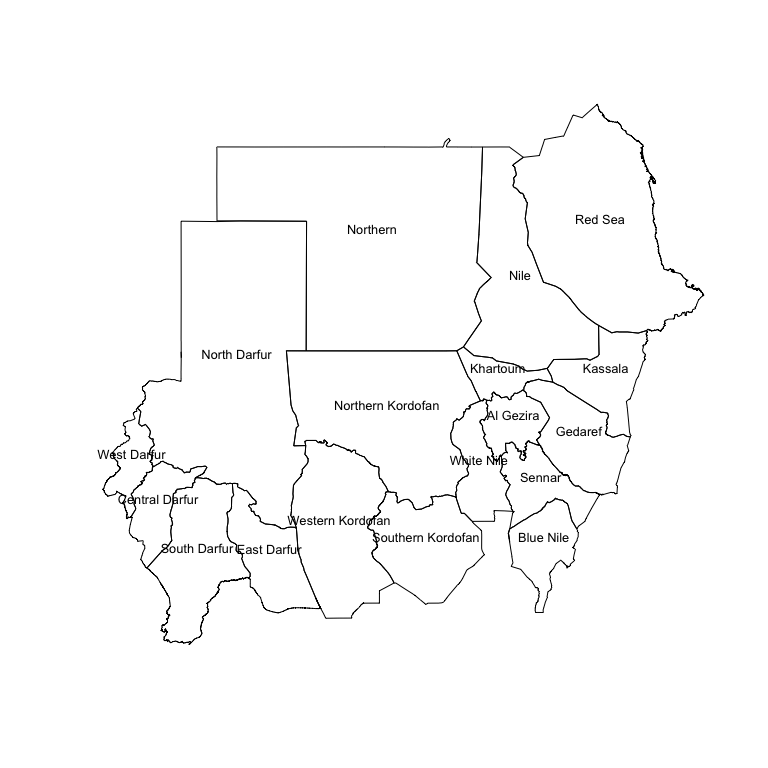
\includegraphics{figures/map6-1} 

}

\caption{Map of states of Sudan with labels}\label{fig:map6}
\end{figure}

\newpage

Now we shall add a \emph{legend} on the map.

We use the \texttt{legend()} function for this. Following are the
commands to create a \emph{legend} for the map of \texttt{sudan01},
\texttt{sudan02} and \texttt{villages}.

~

\begin{Shaded}
\begin{Highlighting}[]
\KeywordTok{plot}\NormalTok{(sudan02, }\DataTypeTok{border =} \StringTok{"gray"}\NormalTok{)}
\KeywordTok{plot}\NormalTok{(sudan01, }\DataTypeTok{lwd =} \DecValTok{2}\NormalTok{, }\DataTypeTok{add =} \OtherTok{TRUE}\NormalTok{)}
\KeywordTok{points}\NormalTok{(villages}\OperatorTok{$}\NormalTok{X, }
\NormalTok{       villages}\OperatorTok{$}\NormalTok{Y, }
       \DataTypeTok{pch =} \DecValTok{20}\NormalTok{, }
       \DataTypeTok{cex =} \FloatTok{0.2}\NormalTok{, }
       \DataTypeTok{col =} \StringTok{"gray90"}\NormalTok{)}
\KeywordTok{legend}\NormalTok{(}\StringTok{"topleft"}\NormalTok{,}
       \DataTypeTok{y.intersp =} \FloatTok{1.2}\NormalTok{,}
       \DataTypeTok{legend =} \KeywordTok{c}\NormalTok{(}\StringTok{"state borders"}\NormalTok{, }\StringTok{"locality borders"}\NormalTok{, }\StringTok{"villages"}\NormalTok{),}
       \DataTypeTok{lty =} \KeywordTok{c}\NormalTok{(}\DecValTok{1}\NormalTok{, }\DecValTok{1}\NormalTok{, }\OtherTok{NA}\NormalTok{),}
       \DataTypeTok{lwd =} \KeywordTok{c}\NormalTok{(}\DecValTok{2}\NormalTok{, }\DecValTok{1}\NormalTok{, }\OtherTok{NA}\NormalTok{),}
       \DataTypeTok{pch =} \KeywordTok{c}\NormalTok{(}\OtherTok{NA}\NormalTok{, }\OtherTok{NA}\NormalTok{, }\DecValTok{20}\NormalTok{),}
       \DataTypeTok{col =} \KeywordTok{c}\NormalTok{(}\StringTok{"black"}\NormalTok{, }\StringTok{"gray"}\NormalTok{, }\StringTok{"gray90"}\NormalTok{),}
       \DataTypeTok{cex =} \FloatTok{0.65}\NormalTok{,}
       \DataTypeTok{pt.cex =} \DecValTok{1}\NormalTok{,}
       \DataTypeTok{bty =} \StringTok{"o"}\NormalTok{,}
       \DataTypeTok{bg =} \StringTok{"white"}\NormalTok{)}
\end{Highlighting}
\end{Shaded}

\newpage

This produces the following map:

~

\begin{figure}[H]

{\centering 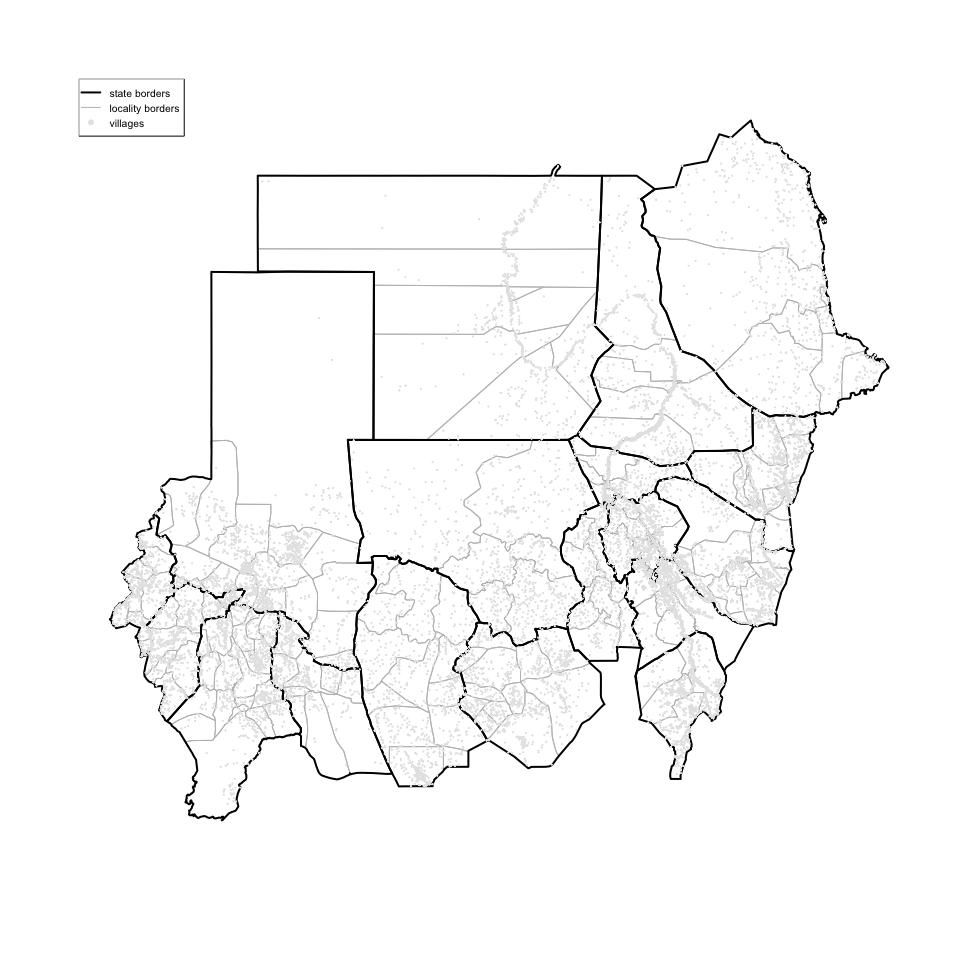
\includegraphics{figures/map7-1} 

}

\caption{Map of localities, states and villages of Sudan with labels and legend}\label{fig:map7}
\end{figure}

\newpage

Lastly, we add a \emph{scale} to our map.

We use the \texttt{map.scale()} function for this. We need to install
and load the library \texttt{maps} to use this function. We add the
scale on the map through the following commands:

~

\begin{Shaded}
\begin{Highlighting}[]
\KeywordTok{plot}\NormalTok{(sudan02, }\DataTypeTok{border =} \StringTok{"gray"}\NormalTok{)}
\KeywordTok{plot}\NormalTok{(sudan01, }\DataTypeTok{lwd =} \DecValTok{2}\NormalTok{, }\DataTypeTok{add =} \OtherTok{TRUE}\NormalTok{)}
\KeywordTok{points}\NormalTok{(villages}\OperatorTok{$}\NormalTok{X, villages}\OperatorTok{$}\NormalTok{Y, }\DataTypeTok{pch =} \DecValTok{20}\NormalTok{, }\DataTypeTok{cex =} \FloatTok{0.2}\NormalTok{, }\DataTypeTok{col =} \StringTok{"gray90"}\NormalTok{)}
\KeywordTok{legend}\NormalTok{(}\StringTok{"topleft"}\NormalTok{,}
       \DataTypeTok{y.intersp =} \FloatTok{1.2}\NormalTok{,}
       \DataTypeTok{legend =} \KeywordTok{c}\NormalTok{(}\StringTok{"state borders"}\NormalTok{, }\StringTok{"locality borders"}\NormalTok{, }\StringTok{"villages"}\NormalTok{),}
       \DataTypeTok{lty =} \KeywordTok{c}\NormalTok{(}\DecValTok{1}\NormalTok{, }\DecValTok{1}\NormalTok{, }\OtherTok{NA}\NormalTok{),}
       \DataTypeTok{lwd =} \KeywordTok{c}\NormalTok{(}\DecValTok{2}\NormalTok{, }\DecValTok{1}\NormalTok{, }\OtherTok{NA}\NormalTok{),}
       \DataTypeTok{pch =} \KeywordTok{c}\NormalTok{(}\OtherTok{NA}\NormalTok{, }\OtherTok{NA}\NormalTok{, }\DecValTok{20}\NormalTok{),}
       \DataTypeTok{col =} \KeywordTok{c}\NormalTok{(}\StringTok{"black"}\NormalTok{, }\StringTok{"gray"}\NormalTok{, }\StringTok{"gray90"}\NormalTok{),}
       \DataTypeTok{cex =} \FloatTok{0.65}\NormalTok{,}
       \DataTypeTok{pt.cex =} \DecValTok{1}\NormalTok{,}
       \DataTypeTok{bty =} \StringTok{"o"}\NormalTok{,}
       \DataTypeTok{bg =} \StringTok{"white"}\NormalTok{)}
\KeywordTok{map.scale}\NormalTok{(}\DataTypeTok{x =} \KeywordTok{bbox}\NormalTok{(sudan01)[}\DecValTok{1}\NormalTok{,], }
          \DataTypeTok{y =} \KeywordTok{bbox}\NormalTok{(sudan01)[}\DecValTok{2}\NormalTok{,],}
          \DataTypeTok{ratio =} \OtherTok{TRUE}\NormalTok{, }
          \DataTypeTok{cex =} \FloatTok{0.65}\NormalTok{)}
\end{Highlighting}
\end{Shaded}

\newpage

This produces the following map:

~

\begin{figure}[H]

{\centering 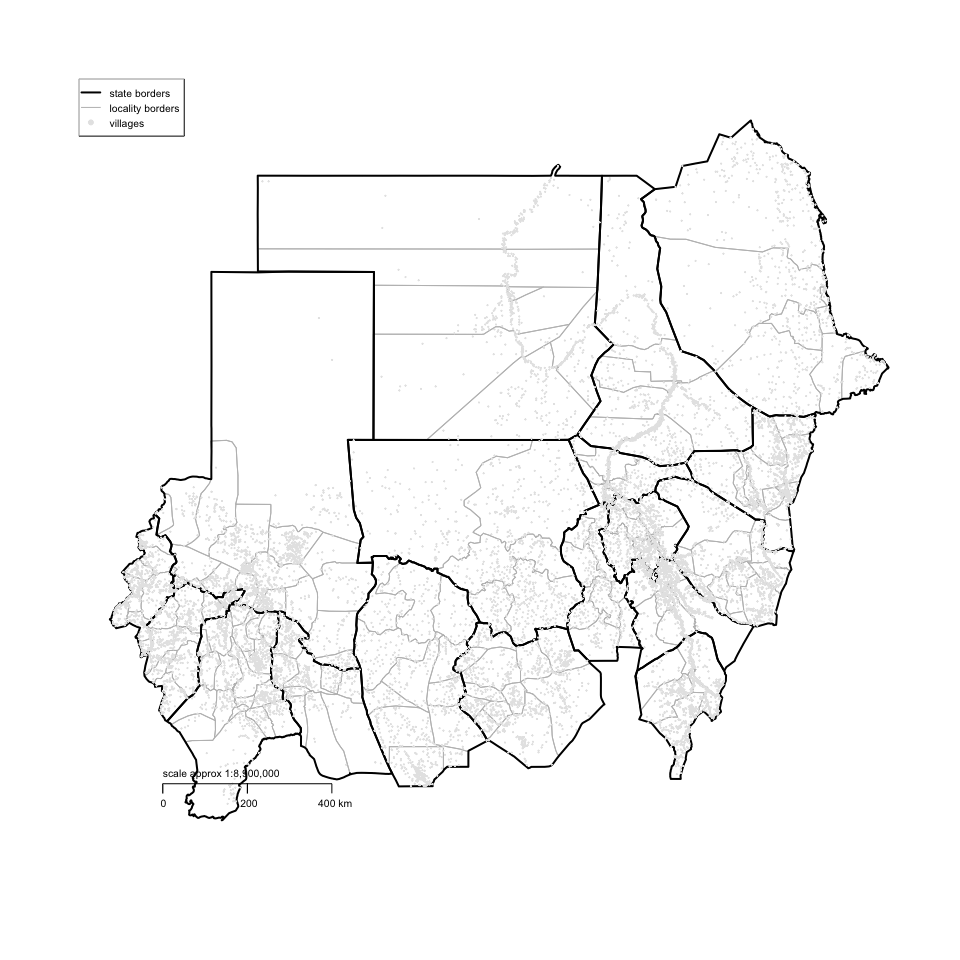
\includegraphics{figures/map8-1} 

}

\caption{Map of localities, states and villages of Sudan with labels, legend and scale}\label{fig:map8}
\end{figure}

\hypertarget{exercise3}{%
\chapter{Manipulating shapefile data}\label{exercise3}}

In this exercise, we will use what we have learned about the structure
and features of shapefile data in manipulating the data and creating new
map objects.

By now you would have noticed that sudan01 and sudan02 shapefile objects
contain data for the whole of Sudan. This is useful for creating maps
for the whole country. However, there are times when we would like to
create maps of the specific states only or assign colours for certain
states differently rather than a single colour for all states.

To do these maps does not require new shapefiles for each of the state.
All this needs is some manipulation of the full country map dataset.
This is possible because the data structure of shapefiles contains all
the data required to map all the features of the overall map separately.

First, let us try to create a map of sudan01 and sudan02 with the states
and the localities coloured differently from each other.

A colour palette should be created which would provide colours for each
of the states. This can be done using the following commands:

~

\begin{Shaded}
\begin{Highlighting}[]
\NormalTok{createPalette <-}\StringTok{ }\KeywordTok{colorRampPalette}\NormalTok{(}\DataTypeTok{colors =} \KeywordTok{c}\NormalTok{(}\StringTok{"#FBB4AE"}\NormalTok{, }\StringTok{"#B3CDE3"}\NormalTok{, }\StringTok{"#CCEBC5"}\NormalTok{, }
                                             \StringTok{"#DECBE4"}\NormalTok{, }\StringTok{"#FED9A6"}\NormalTok{, }\StringTok{"#FFFFCC"}\NormalTok{, }
                                             \StringTok{"#E5D8BD"}\NormalTok{, }\StringTok{"#FDDAEC"}\NormalTok{, }\StringTok{"#F2F2F2"}\NormalTok{), }
                                  \DataTypeTok{space =} \StringTok{"Lab"}\NormalTok{)}
\NormalTok{sudanCol <-}\StringTok{ }\KeywordTok{createPalette}\NormalTok{(}\DecValTok{18}\NormalTok{)}
\end{Highlighting}
\end{Shaded}

~

What this command uses the \texttt{colorRampPalette()} function to
create a colour palette of 18 unique colours (one for each state). These
colours were generated from a base set of 9 colours which in turn was
chosen using a qualitative colour scheme from ColorBrewer 2.0 (see
\url{http://www.colorbrewer2.org}).

\newpage

Once we have a colour palette to use, we now plot the map and use the
colour palette to specify the parameter col. This is done as follows:

~

\begin{Shaded}
\begin{Highlighting}[]
\KeywordTok{plot}\NormalTok{(sudan01, }\DataTypeTok{border =}\NormalTok{ sudanCol, }\DataTypeTok{col =}\NormalTok{ sudanCol)}
\KeywordTok{plot}\NormalTok{(sudan02, }\DataTypeTok{lwd =} \FloatTok{0.5}\NormalTok{, }\DataTypeTok{lty =} \DecValTok{3}\NormalTok{, }\DataTypeTok{border =} \StringTok{"gray"}\NormalTok{, }\DataTypeTok{add =} \OtherTok{TRUE}\NormalTok{)}
\KeywordTok{plot}\NormalTok{(sudan01, }\DataTypeTok{lwd =} \DecValTok{1}\NormalTok{, }\DataTypeTok{border =} \StringTok{"gray"}\NormalTok{, }\DataTypeTok{add =} \OtherTok{TRUE}\NormalTok{)}
\KeywordTok{text}\NormalTok{(}\DataTypeTok{x =} \KeywordTok{coordinates}\NormalTok{(sudan01)[,}\DecValTok{1}\NormalTok{], }
     \DataTypeTok{y =} \KeywordTok{coordinates}\NormalTok{(sudan01)[,}\DecValTok{2}\NormalTok{],}
     \DataTypeTok{labels =}\NormalTok{ sudan01}\OperatorTok{@}\NormalTok{data}\OperatorTok{$}\NormalTok{State, }
     \DataTypeTok{pos =} \DecValTok{3}\NormalTok{, }
     \DataTypeTok{offset =} \FloatTok{0.2}\NormalTok{, }
     \DataTypeTok{cex =} \DecValTok{1}\NormalTok{)}
\end{Highlighting}
\end{Shaded}

\newpage

The resulting map is:

~

\begin{figure}[H]

{\centering 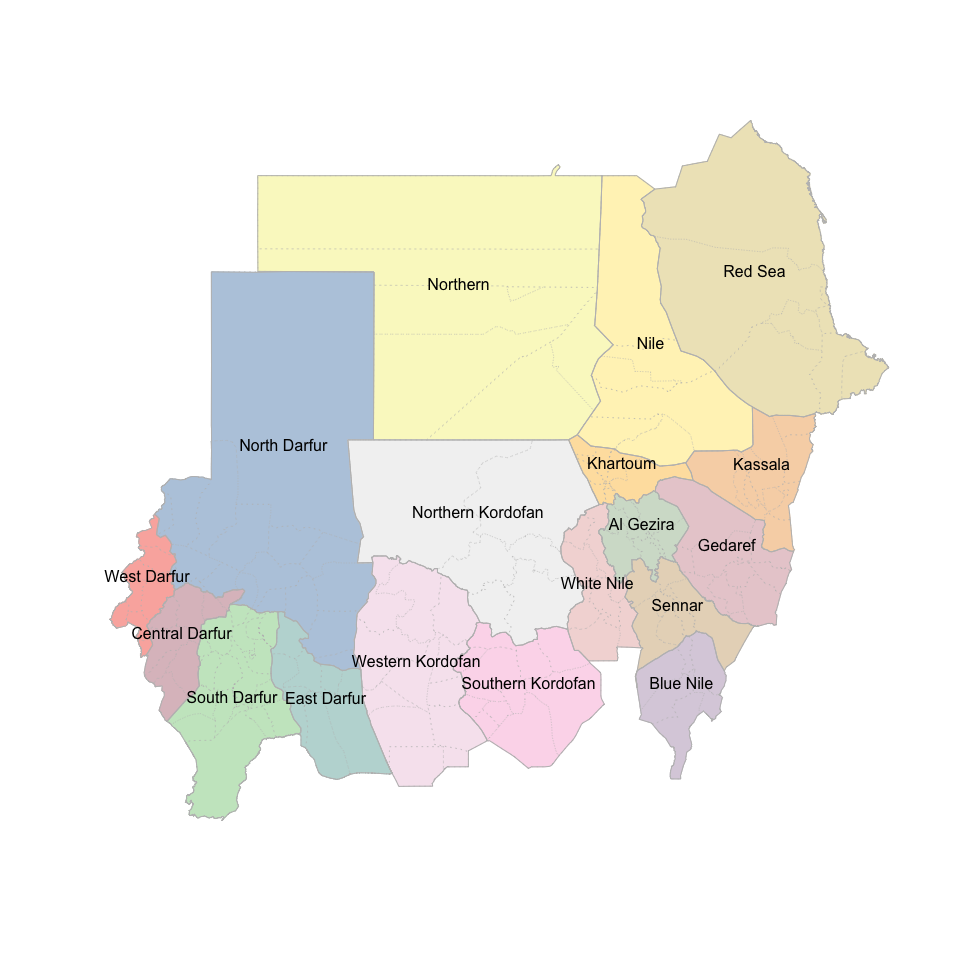
\includegraphics{figures/map9-1} 

}

\caption{Map of localities and states of Sudan coloured }\label{fig:map9}
\end{figure}

\newpage

Now, let us try to specify a colour to just a handful of the states
while the others remain without colour. This is particularly useful when
you just want to highlight specific states in the map for presentation
purpose or for emphasis.

For this map, we will need to use the
\href{mailto:sudan01@data}{\nolinkurl{sudan01@data}} slot to steer our
selection of the states of interest which we can then specify a colour
for. For example, if we want to show the full Sudan map and Gedaref,
Northern and Western Kordofan coloured light green, we call the
following commands:

~

\begin{Shaded}
\begin{Highlighting}[]
\KeywordTok{plot}\NormalTok{(sudan01, }
     \DataTypeTok{lty =} \DecValTok{0}\NormalTok{, }
     \DataTypeTok{col =} \KeywordTok{ifelse}\NormalTok{(sudan01}\OperatorTok{@}\NormalTok{data}\OperatorTok{$}\NormalTok{State }\OperatorTok\StringTok{ }\KeywordTok{c}\NormalTok{(}\StringTok{"Gedaref"}\NormalTok{, }
                                            \StringTok{"Northern"}\NormalTok{, }
                                            \StringTok{"Western Kordofan"}\NormalTok{), }
                  \StringTok{"lightgreen"}\NormalTok{, }\OtherTok{NA}\NormalTok{))}
\KeywordTok{plot}\NormalTok{(sudan02, }\DataTypeTok{lwd =} \FloatTok{0.5}\NormalTok{, }\DataTypeTok{lty =} \DecValTok{3}\NormalTok{, }\DataTypeTok{border =} \StringTok{"gray"}\NormalTok{, }\DataTypeTok{add =} \OtherTok{TRUE}\NormalTok{)}
\KeywordTok{plot}\NormalTok{(sudan01, }\DataTypeTok{lwd =} \DecValTok{1}\NormalTok{, }\DataTypeTok{add =} \OtherTok{TRUE}\NormalTok{)}
\KeywordTok{text}\NormalTok{(}\DataTypeTok{x =} \KeywordTok{coordinates}\NormalTok{(sudan01)[,}\DecValTok{1}\NormalTok{], }
     \DataTypeTok{y =} \KeywordTok{coordinates}\NormalTok{(sudan01)[,}\DecValTok{2}\NormalTok{], }
     \DataTypeTok{labels =}\NormalTok{ sudan01}\OperatorTok{@}\NormalTok{data}\OperatorTok{$}\NormalTok{State, }
     \DataTypeTok{pos =} \DecValTok{3}\NormalTok{, }
     \DataTypeTok{offset =} \FloatTok{0.2}\NormalTok{, }
     \DataTypeTok{cex =} \DecValTok{1}\NormalTok{)}
\end{Highlighting}
\end{Shaded}

\newpage

The resulting map is:

~

\begin{figure}[H]

{\centering 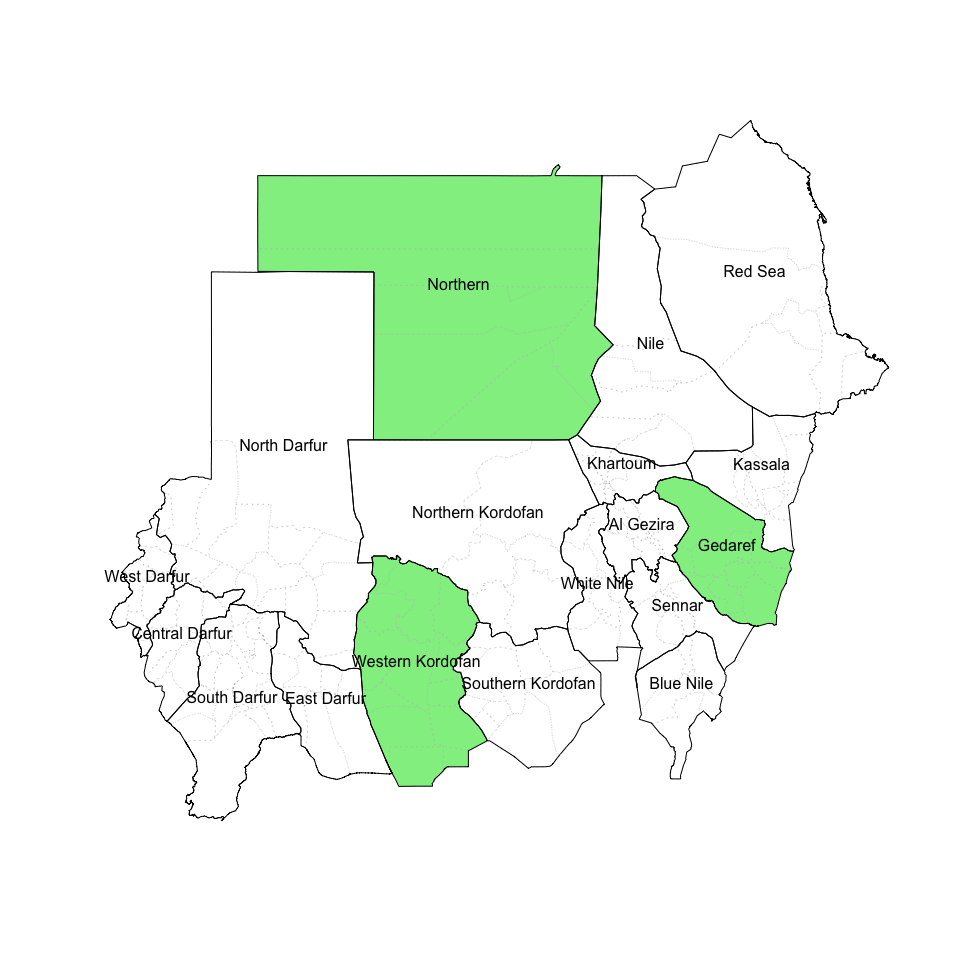
\includegraphics{figures/map10-1} 

}

\caption{Map of specific states of Sudan coloured}\label{fig:map10}
\end{figure}

~

There are practical uses for knowing how to manipulate map data so as to
change the colour of the components polygons either based on a
qualitative criteria (such as different colours for each state to
distinguish them from each other) or on numerical data (such as in
creating a choropleth map).

The following example of simulated CMAM coverage results per state
illustrates this usefullness.

\newpage

We first simulate the data as follows:

~

\begin{Shaded}
\begin{Highlighting}[]
\NormalTok{states   <-}\StringTok{ }\KeywordTok{as.vector}\NormalTok{(sudan01}\OperatorTok{@}\NormalTok{data}\OperatorTok{$}\NormalTok{State)}
\NormalTok{coverage <-}\StringTok{ }\KeywordTok{c}\NormalTok{(}\DecValTok{95}\NormalTok{, }\DecValTok{56}\NormalTok{, }\DecValTok{73}\NormalTok{, }\DecValTok{55}\NormalTok{, }\DecValTok{19}\NormalTok{, }\DecValTok{97}\NormalTok{, }
              \DecValTok{60}\NormalTok{, }\DecValTok{2}\NormalTok{, }\DecValTok{46}\NormalTok{, }\DecValTok{31}\NormalTok{, }\DecValTok{70}\NormalTok{, }\DecValTok{23}\NormalTok{, }
              \DecValTok{71}\NormalTok{, }\DecValTok{66}\NormalTok{, }\DecValTok{38}\NormalTok{, }\DecValTok{78}\NormalTok{, }\DecValTok{74}\NormalTok{, }\DecValTok{51}\NormalTok{)}

\NormalTok{exData <-}\StringTok{ }\KeywordTok{data.frame}\NormalTok{(states, coverage)}
\KeywordTok{names}\NormalTok{(exData) <-}\StringTok{ }\KeywordTok{c}\NormalTok{(}\StringTok{"states"}\NormalTok{, }\StringTok{"coverage"}\NormalTok{) }
\end{Highlighting}
\end{Shaded}

~

The \texttt{exData} object gives us the simulated of CMAM coverage by
state. Then we specify a colour palette as follows:

~

\begin{Shaded}
\begin{Highlighting}[]
\NormalTok{createMapPalette <-}\StringTok{ }\KeywordTok{colorRampPalette}\NormalTok{(}\DataTypeTok{colors =} \KeywordTok{c}\NormalTok{(}\StringTok{"white"}\NormalTok{, }\StringTok{"lightgreen"}\NormalTok{, }
                                                \StringTok{"green"}\NormalTok{, }\StringTok{"darkgreen"}\NormalTok{), }
                                     \DataTypeTok{space =} \StringTok{"Lab"}\NormalTok{)}
\NormalTok{mapPalette <-}\StringTok{ }\KeywordTok{createMapPalette}\NormalTok{(}\DecValTok{101}\NormalTok{)}
\end{Highlighting}
\end{Shaded}

~

We now can map this data using the folowing commands:

~

\begin{Shaded}
\begin{Highlighting}[]
\KeywordTok{plot}\NormalTok{(sudan01, }\DataTypeTok{lty =} \DecValTok{0}\NormalTok{, }\DataTypeTok{col =}\NormalTok{ mapPalette[exData}\OperatorTok{$}\NormalTok{coverage])}
\KeywordTok{plot}\NormalTok{(sudan02, }\DataTypeTok{lwd =} \FloatTok{0.5}\NormalTok{, }\DataTypeTok{lty =} \DecValTok{3}\NormalTok{, }\DataTypeTok{border =} \StringTok{"gray"}\NormalTok{, }\DataTypeTok{add =} \OtherTok{TRUE}\NormalTok{)}
\KeywordTok{plot}\NormalTok{(sudan01, }\DataTypeTok{lwd =} \DecValTok{1}\NormalTok{, }\DataTypeTok{add =} \OtherTok{TRUE}\NormalTok{)}
\KeywordTok{text}\NormalTok{(}\DataTypeTok{x =} \KeywordTok{coordinates}\NormalTok{(sudan01)[,}\DecValTok{1}\NormalTok{], }
     \DataTypeTok{y =} \KeywordTok{coordinates}\NormalTok{(sudan01)[,}\DecValTok{2}\NormalTok{], }
     \DataTypeTok{labels =}\NormalTok{ sudan01}\OperatorTok{@}\NormalTok{data}\OperatorTok{$}\NormalTok{State, }
     \DataTypeTok{pos =} \DecValTok{3}\NormalTok{, }
     \DataTypeTok{offset =} \FloatTok{0.2}\NormalTok{, }
     \DataTypeTok{cex =} \DecValTok{1}\NormalTok{)}
\end{Highlighting}
\end{Shaded}

\newpage

This results in the following map:

~

\begin{figure}[H]

{\centering 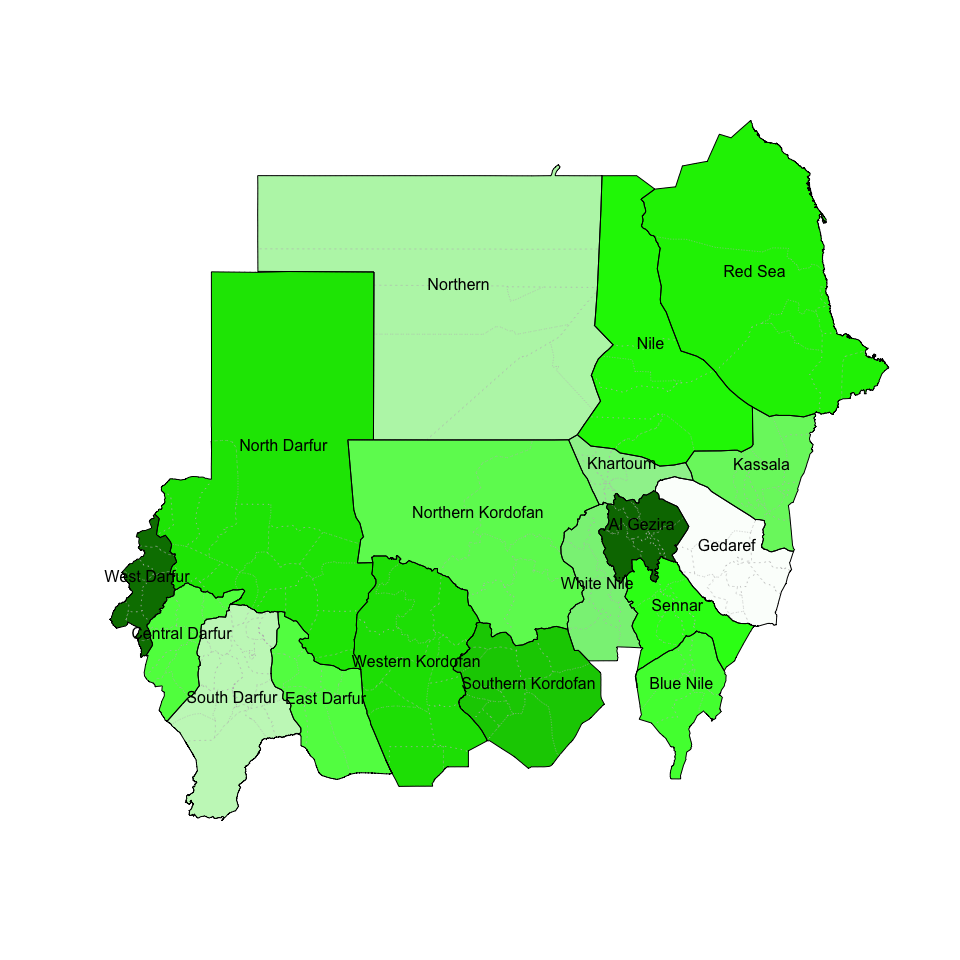
\includegraphics{figures/map11-1} 

}

\caption{Sample coverage map}\label{fig:map11}
\end{figure}

~

Finally, we learn how to create maps for each state separately using the
\texttt{sudan01} map dataset.

To begin with, let's try to create and map a map dataset for North
Darfur. We call the following commands:

~

\begin{Shaded}
\begin{Highlighting}[]
\NormalTok{nDarfur <-}\StringTok{ }\KeywordTok{subset}\NormalTok{(sudan01, sudan01}\OperatorTok{@}\NormalTok{data}\OperatorTok{$}\NormalTok{State }\OperatorTok{==}\StringTok{ "North Darfur"}\NormalTok{)}
\KeywordTok{plot}\NormalTok{(nDarfur)}
\end{Highlighting}
\end{Shaded}

\newpage

To produce the following:

~

\begin{figure}[H]

{\centering 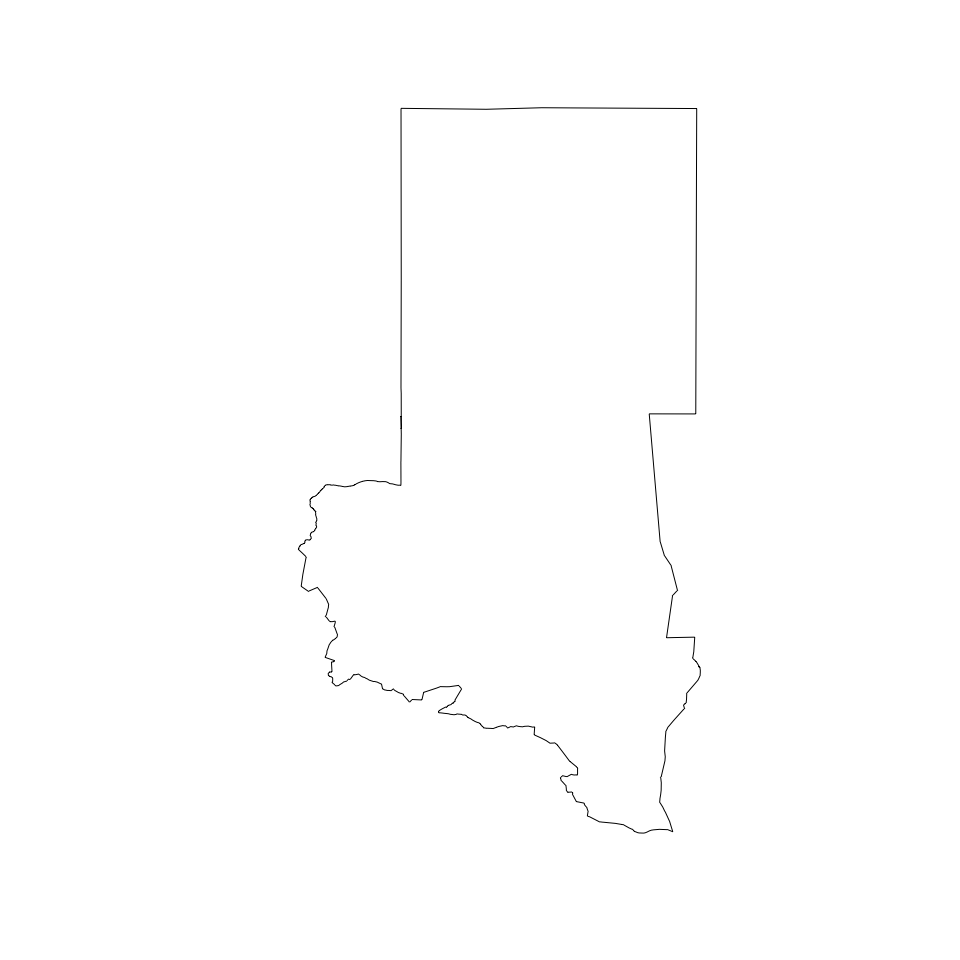
\includegraphics{figures/map12-1} 

}

\caption{Map of North Darfur, Sudan}\label{fig:map12}
\end{figure}

\newpage

However, this map will look better if we can also show the nearby states
and their boundaries. We can do this by plotting \texttt{sudan01} but
this time specifying a \texttt{xlim} and \texttt{ylim} parameters using
the \texttt{bbox()} of the map object for North Darfur. The following
commands illustrate this:

~

\begin{Shaded}
\begin{Highlighting}[]
\NormalTok{nDarfur <-}\StringTok{ }\KeywordTok{subset}\NormalTok{(sudan01, sudan01}\OperatorTok{@}\NormalTok{data}\OperatorTok{$}\NormalTok{State }\OperatorTok{==}\StringTok{ "North Darfur"}\NormalTok{)}
\NormalTok{ndLimits <-}\StringTok{ }\KeywordTok{bbox}\NormalTok{(nDarfur)}
\KeywordTok{plot}\NormalTok{(sudan01, }
     \DataTypeTok{xlim =}\NormalTok{ ndLimits[}\DecValTok{1}\NormalTok{,], }
     \DataTypeTok{ylim =}\NormalTok{ ndLimits[}\DecValTok{2}\NormalTok{,], }
     \DataTypeTok{border =} \StringTok{"gray"}\NormalTok{)}
\KeywordTok{plot}\NormalTok{(nDarfur, }
     \DataTypeTok{xlim =}\NormalTok{ ndLimits[}\DecValTok{1}\NormalTok{,], }
     \DataTypeTok{ylim =}\NormalTok{ ndLimits[}\DecValTok{2}\NormalTok{,], }
     \DataTypeTok{border =} \StringTok{"blue"}\NormalTok{, }
     \DataTypeTok{add =} \OtherTok{TRUE}\NormalTok{)}
\end{Highlighting}
\end{Shaded}

\newpage

The resulting map is:

~

\begin{figure}[H]

{\centering 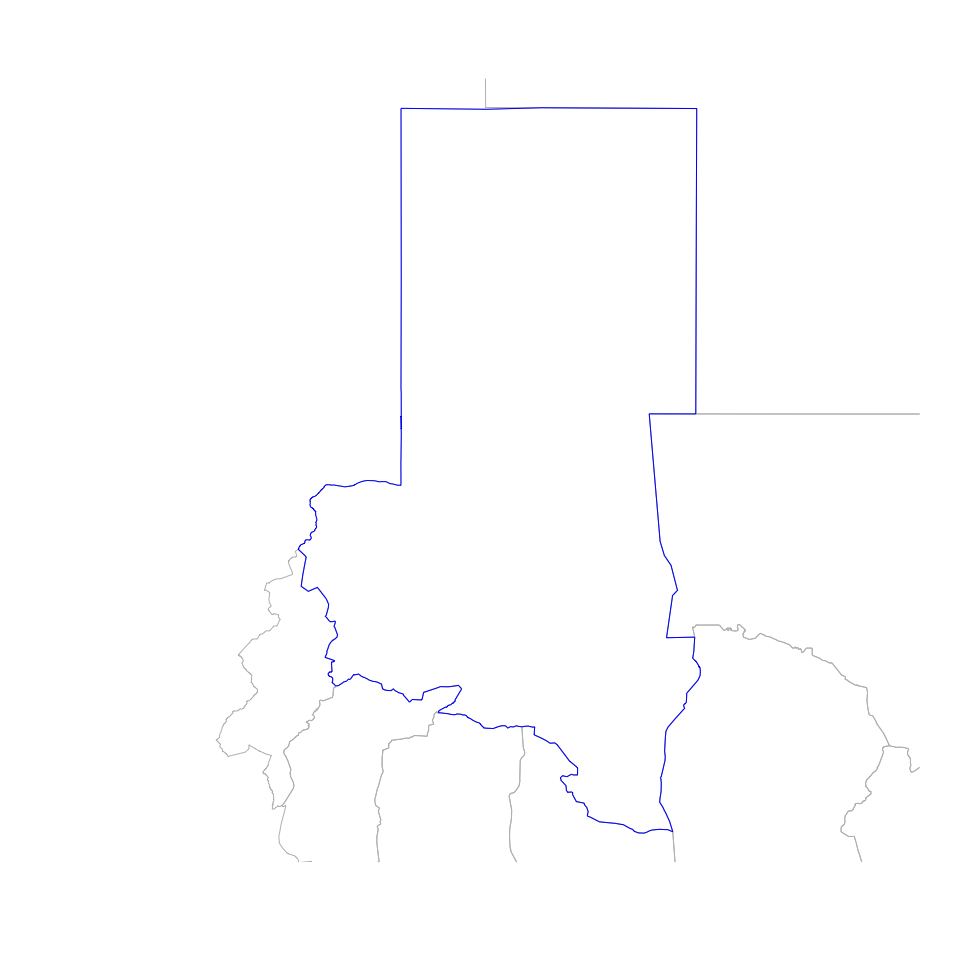
\includegraphics{figures/map13-1} 

}

\caption{Map of North Darfur, Sudan}\label{fig:map13}
\end{figure}

~

We can apply the same approach to get the map for each of the states.
However, we can also create a looping function that will create and plot
the maps for us automatically. This can be done as follows:

~

\begin{Shaded}
\begin{Highlighting}[]
\NormalTok{stateList <-}\StringTok{ }\KeywordTok{as.vector}\NormalTok{(sudan01}\OperatorTok{@}\NormalTok{data}\OperatorTok{$}\NormalTok{State)}

\ControlFlowTok{for}\NormalTok{(i }\ControlFlowTok{in} \DecValTok{1}\OperatorTok{:}\KeywordTok{nrow}\NormalTok{(sudan01}\OperatorTok{@}\NormalTok{data)) \{}
\NormalTok{  a <-}\StringTok{ }\KeywordTok{subset}\NormalTok{(sudan01, sudan01}\OperatorTok{@}\NormalTok{data}\OperatorTok{$}\NormalTok{State }\OperatorTok{==}\StringTok{ }\NormalTok{stateList[i])}
  
\NormalTok{  aLimits <-}\StringTok{ }\KeywordTok{bbox}\NormalTok{(a)}
  
  \KeywordTok{plot}\NormalTok{(sudan01, }
       \DataTypeTok{xlim =}\NormalTok{ aLimits[}\DecValTok{1}\NormalTok{,], }
       \DataTypeTok{ylim =}\NormalTok{ aLimits[}\DecValTok{2}\NormalTok{,], }
       \DataTypeTok{border =} \StringTok{"gray"}\NormalTok{)}
  
  \KeywordTok{plot}\NormalTok{(a, }
       \DataTypeTok{xlim =}\NormalTok{ aLimits[}\DecValTok{1}\NormalTok{,], }
       \DataTypeTok{ylim =}\NormalTok{ aLimits[}\DecValTok{2}\NormalTok{,], }
       \DataTypeTok{border =} \StringTok{"blue"}\NormalTok{, }
       \DataTypeTok{add =} \OtherTok{TRUE}\NormalTok{)}
  
  \KeywordTok{points}\NormalTok{(villages}\OperatorTok{$}\NormalTok{X, villages}\OperatorTok{$}\NormalTok{Y, }\DataTypeTok{pch =} \DecValTok{20}\NormalTok{, }\DataTypeTok{cex =} \FloatTok{0.3}\NormalTok{, }\DataTypeTok{col =} \StringTok{"gray90"}\NormalTok{)}
  
  \KeywordTok{title}\NormalTok{(}\DataTypeTok{main =}\NormalTok{ stateList[i], }\DataTypeTok{cex =} \DecValTok{2}\NormalTok{)}
\NormalTok{\}}
\end{Highlighting}
\end{Shaded}

\newpage

The commands above will create a plot of the individual state maps on
separate graphics device which can be saved one by one. An example of
the maps is below.

~

\begin{figure}[H]

{\centering 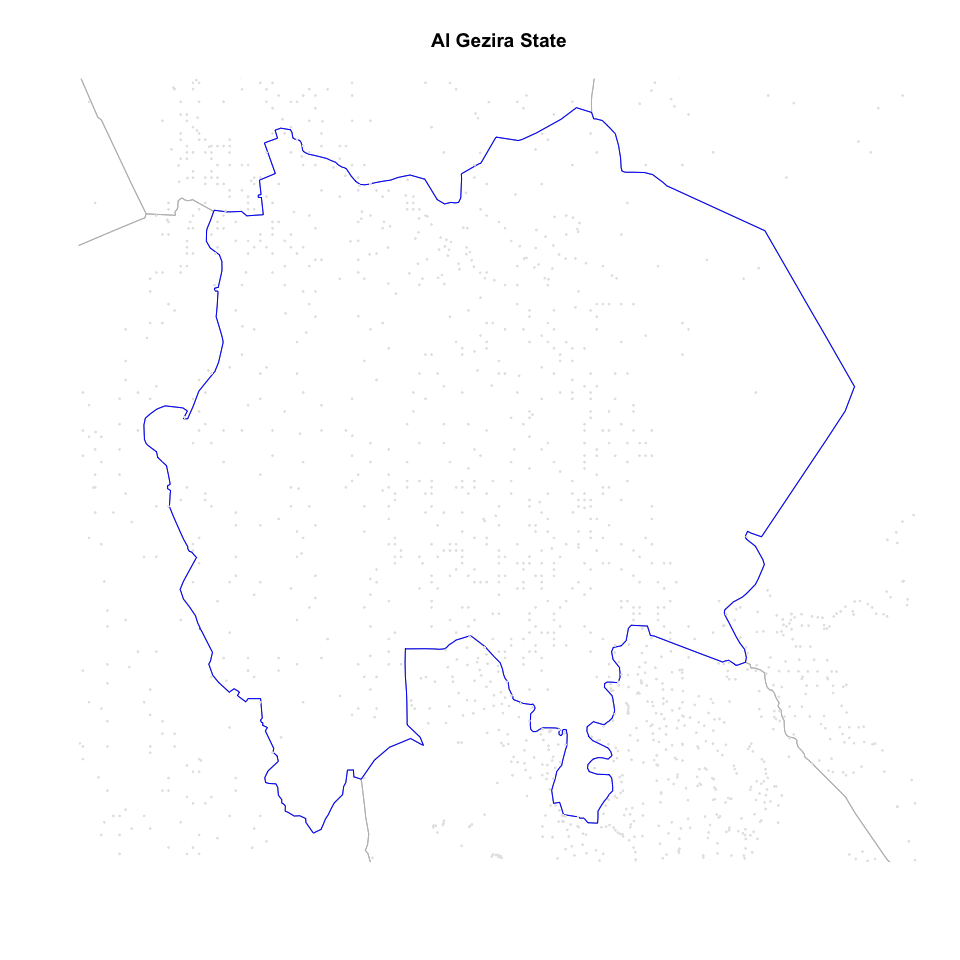
\includegraphics{figures/map14-1} 

}

\caption{Map of Al Gezira State, Sudan}\label{fig:map14}
\end{figure}

\newpage

The other approach is to plot each of the individual state map on the
same graphics device. This can be done using the following commands:

~

\begin{Shaded}
\begin{Highlighting}[]
\NormalTok{stateList <-}\StringTok{ }\KeywordTok{as.vector}\NormalTok{(sudan01}\OperatorTok{@}\NormalTok{data}\OperatorTok{$}\NormalTok{State)}

\KeywordTok{par}\NormalTok{(}\DataTypeTok{mar =} \KeywordTok{c}\NormalTok{(}\DecValTok{2}\NormalTok{,}\DecValTok{2}\NormalTok{,}\DecValTok{2}\NormalTok{,}\DecValTok{2}\NormalTok{)); }\KeywordTok{par}\NormalTok{(}\DataTypeTok{mfrow =} \KeywordTok{c}\NormalTok{(}\DecValTok{6}\NormalTok{,}\DecValTok{3}\NormalTok{))}

\ControlFlowTok{for}\NormalTok{(i }\ControlFlowTok{in} \DecValTok{1}\OperatorTok{:}\KeywordTok{nrow}\NormalTok{(sudan01}\OperatorTok{@}\NormalTok{data)) \{}
\NormalTok{  a <-}\StringTok{ }\KeywordTok{subset}\NormalTok{(sudan01, sudan01}\OperatorTok{@}\NormalTok{data}\OperatorTok{$}\NormalTok{State }\OperatorTok{==}\StringTok{ }\NormalTok{stateList[i])}
\NormalTok{  aLimits <-}\StringTok{ }\KeywordTok{bbox}\NormalTok{(a)}
    
  \KeywordTok{plot}\NormalTok{(sudan01, }
       \DataTypeTok{xlim =}\NormalTok{ aLimits[}\DecValTok{1}\NormalTok{,], }
       \DataTypeTok{ylim =}\NormalTok{ aLimits[}\DecValTok{2}\NormalTok{,], }
       \DataTypeTok{border =} \StringTok{"gray"}\NormalTok{)}
      
  \KeywordTok{plot}\NormalTok{(a, }
       \DataTypeTok{xlim =}\NormalTok{ aLimits[}\DecValTok{1}\NormalTok{,], }
       \DataTypeTok{ylim =}\NormalTok{ aLimits[}\DecValTok{2}\NormalTok{,], }
       \DataTypeTok{lwd =} \DecValTok{2}\NormalTok{, }
       \DataTypeTok{border =} \StringTok{"blue"}\NormalTok{, }
       \DataTypeTok{add =} \OtherTok{TRUE}\NormalTok{)}
  
  \KeywordTok{points}\NormalTok{(}\DataTypeTok{x =}\NormalTok{ villages}\OperatorTok{$}\NormalTok{X, }
         \DataTypeTok{y =}\NormalTok{ villages}\OperatorTok{$}\NormalTok{Y, }
         \DataTypeTok{pch =} \DecValTok{20}\NormalTok{, }
         \DataTypeTok{cex =} \FloatTok{0.3}\NormalTok{, }
         \DataTypeTok{col =} \StringTok{"gray90"}\NormalTok{)}
  
  \KeywordTok{title}\NormalTok{(}\DataTypeTok{main =} \KeywordTok{paste}\NormalTok{(stateList[i], }\StringTok{"State"}\NormalTok{, }\DataTypeTok{sep =} \StringTok{" "}\NormalTok{), }\DataTypeTok{cex =} \DecValTok{2}\NormalTok{)}
\NormalTok{\}}
\end{Highlighting}
\end{Shaded}

~

The resulting map is:

~

\begin{figure}[H]

{\centering 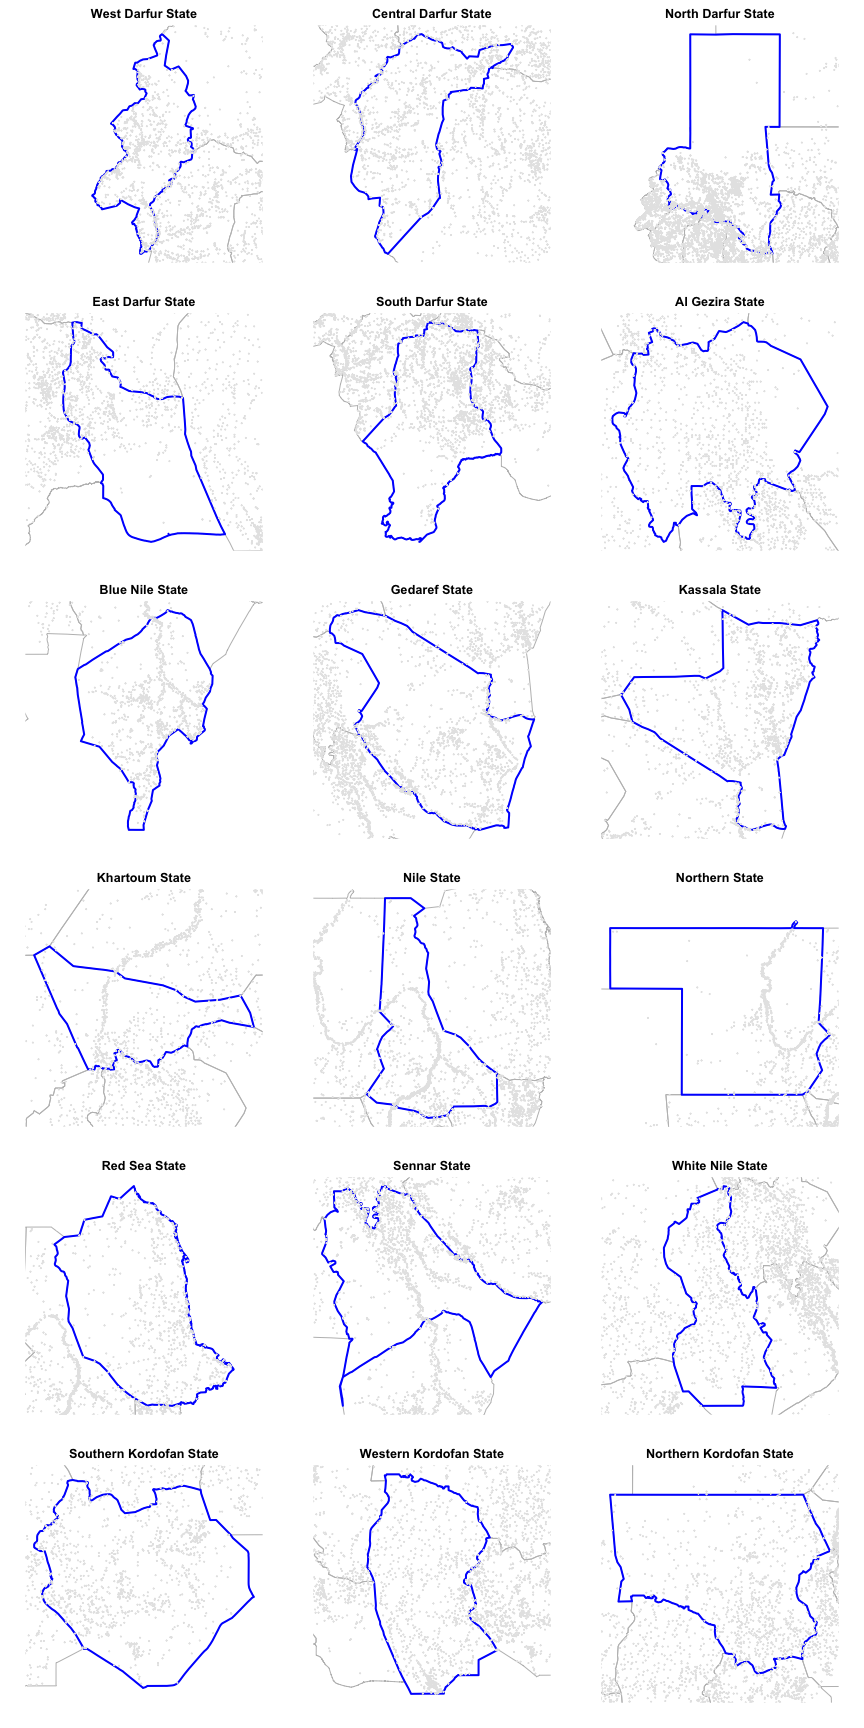
\includegraphics{figures/map15-1} 

}

\caption{Map for each state of Sudan}\label{fig:map15}
\end{figure}

\bibliography{book.bib}


\end{document}
